\documentclass[letterpaper,10pt,onecolumn]{IEEEtran}
\usepackage[margin=0.75in]{geometry}

\usepackage[final]{pdfpages}
\usepackage{breakcites}
\usepackage{graphicx}
\usepackage{amssymb}
\usepackage{amsmath}
\usepackage{amsthm}
\usepackage{cite}
\usepackage{alltt}
\usepackage{float}
\usepackage{color}
\usepackage{url}
\usepackage{titling}
\usepackage{balance}
\usepackage[subfigure]{tocloft} 
\usepackage{subfigure} 
\usepackage{enumitem}
\usepackage{pstricks, pst-node}
\usepackage{listings}
\usepackage{color}
\usepackage{tabularx}
\usepackage{textcomp}
\usepackage{pgfgantt}
\usepackage{hyperref}
\usepackage{changepage}
\renewcommand{\cftsecleader}{\cftdotfill{\cftdotsep}}
%% The following metadata will show up in the PDF properties
\def\title{Computer Science Senior Software Engineering Project (CS463)}
\def\name{Krisna Irawan\\ Jiongcheng Luo\\ Drew Hamm}
\def\doc{Final Report}
\def\term{Spring 2017}
\def\project{Head-Up Display Alignment System}

% code color highlight setup
\definecolor{mygreen}{rgb}{0,0.6,0}
\definecolor{mygray}{rgb}{0.5,0.5,0.5}
\definecolor{mymauve}{rgb}{0.58,0,0.82}

\lstset{ %
  backgroundcolor=\color{black!3},   % choose the background color
  basicstyle=\footnotesize,        % size of fonts used for the code
  breaklines=true,                 % automatic line breaking only at whitespace
  captionpos=b,                    % sets the caption-position to bottom
  commentstyle=\color{mygreen},    % comment style
  escapeinside={\%*}{*)},          % if you want to add LaTeX within your code
  keywordstyle=\color{blue},       % keyword style
  stringstyle=\color{mymauve},     % string literal style
  language=C++
}

\hypersetup{
  colorlinks = true,
  urlcolor = black,
  linkcolor  = black,
  pdfauthor = {\name},
  pdfkeywords = {capstone, \doc},
  pdftitle = {\doc},
  pdfsubject = {\doc},
  pdfpagemode = UseNone
}


% define figure directory path 
\graphicspath {{images/}}
\begin{document}

\begin{titlepage}
\centering
	\begin{figure}
      	
\includegraphics[scale=0.25]{osu_logo}
	\end{figure}
	{\Large\itshape \title\par}
	\vspace{1.5cm}
	\scshape{
		{\Huge \project\par}

		\vspace{1.5cm}
		{\Huge\bfseries\doc\par}
		{\huge \term\par}
	}
	\vspace{2cm}
	{\large\itshape\bfseries Group 65:\par}
	{\large \name\par}
	\vspace{2cm}
	{\large\itshape\bfseries Sponsor:\par}
	{\large Rockwell Collins, Inc.\par}
	\vspace{2cm}
	{\large \today\par}
	\vspace{2cm}

	% ============= Abstract =================
	\begin{abstract}
		This document reports the progress that we have made since the beginning of spring term of 2017. This report mainly introduces our current progress and remaining works of the project, problems that we encoutered and their solutions. This report will also cover the highlighted codes of the software as well as a prelimary result of this project.
	\end{abstract}
	\vfill

\end{titlepage}
\tableofcontents

\newpage

\section{Introduction}
\subsection{Purpose}
The purpose of this software design document is to provide a description that sufficiently describes the system design. The system design must be specified completely to the point in which is needed for the development to proceed. The description will fully specify what is to be built, how it will be built and what expectations need to be met at completion.

\subsection{Purpose}
A HUD or a Head-Up Display provides critical information to the pilots during flight environment. Currently, the HUD obtains data from an aircraft’s mounted device called an Inertial Reference Unit (IRU), which an IRU would output precise and aligned data to the HUD through an mechanical alignment system. However, the current alignment process requires specialized equipment and epoxy which is time consuming, costly, and interrupts production line progress for the original equipment manufacturer. In addition, the resulting HUD alignment, while precise, does not compensate for airframe droop during flight. Rockwell Collins looks forward to a new alignment methodology utilizing an inexpensive microelectromechanical systems (MEMS) IRU mounted onto the HUD to infer alignment data from the aircraft’s precisely mounted and aligned IRU.

This project is to develop a feasible demonstration system as a proof of concept for Rockwell Collins, that will prove there is an algorithm that is able to output precise and aligned data with reduced installation cost utilizing the data from both the inexpensive MEMS IRU and the aircraft mounted IRU. The outcome (aligned-data) of this algorithm will compensate the alignment error correctly, and the alignment error should be within a range of one milliradian. The product will make the alignment process more dynamic and less time consuming. The dynamic alignment process also makes this new system compensate for the airframe droop that happens during the flight environment. As well as from the perspective of the industries, this product aims to improve the installation process by reducing cost and time for all parties involved.

\subsection{Overview}
The following second and third part of this document are glossary and references that we have for this document. The fourth part of this document cover the design and implementation details of this project. The design and implementation details of this document are split into six different viewpoints. These viewpoints contain context view, composition view, dependency view, interface view, interaction view, and algorithm view. 

\newpage
\section{Original Requirements Document}
\def\RDtitle{Computer Science Senior Software Engineering Project (CS462)}
\def\RDversion{2.0}
\def\RDterm{Winter 2017}

	\centering
	\vspace{\fill}

	{\Huge\bfseries Original Requirements Document\par}
	\vspace{0.5cm}
	{\Large\itshape \RDtitle\par}
	\vspace{0.5cm}
	{\Large\itshape \RDterm\par}
	
	\vspace{\fill}
	
	\begin{abstract}
	We are working with Rockwell Collins to explore potential technological innovations relating to their Head-Up Display (HUD) systems that present critical flight information to pilots. Our primary objective is to improve Rockwell Collins current HUD systems by reducing the cost and time required to precisely align flight information to the HUD. To meet our objective we will look into using a new alignment methodology in conjunction with the current HUD system as a proof of concept. The product being developed is a demonstration system that looks to include a MEMS IRU mounted onto the HUD and a new alignment algorithm that utilizes this additional sensor to determine accurate HUD alignment. This document will introduce the specific details of the demonstration system and describe the requirements for the development of the product.
	\end{abstract}
	
	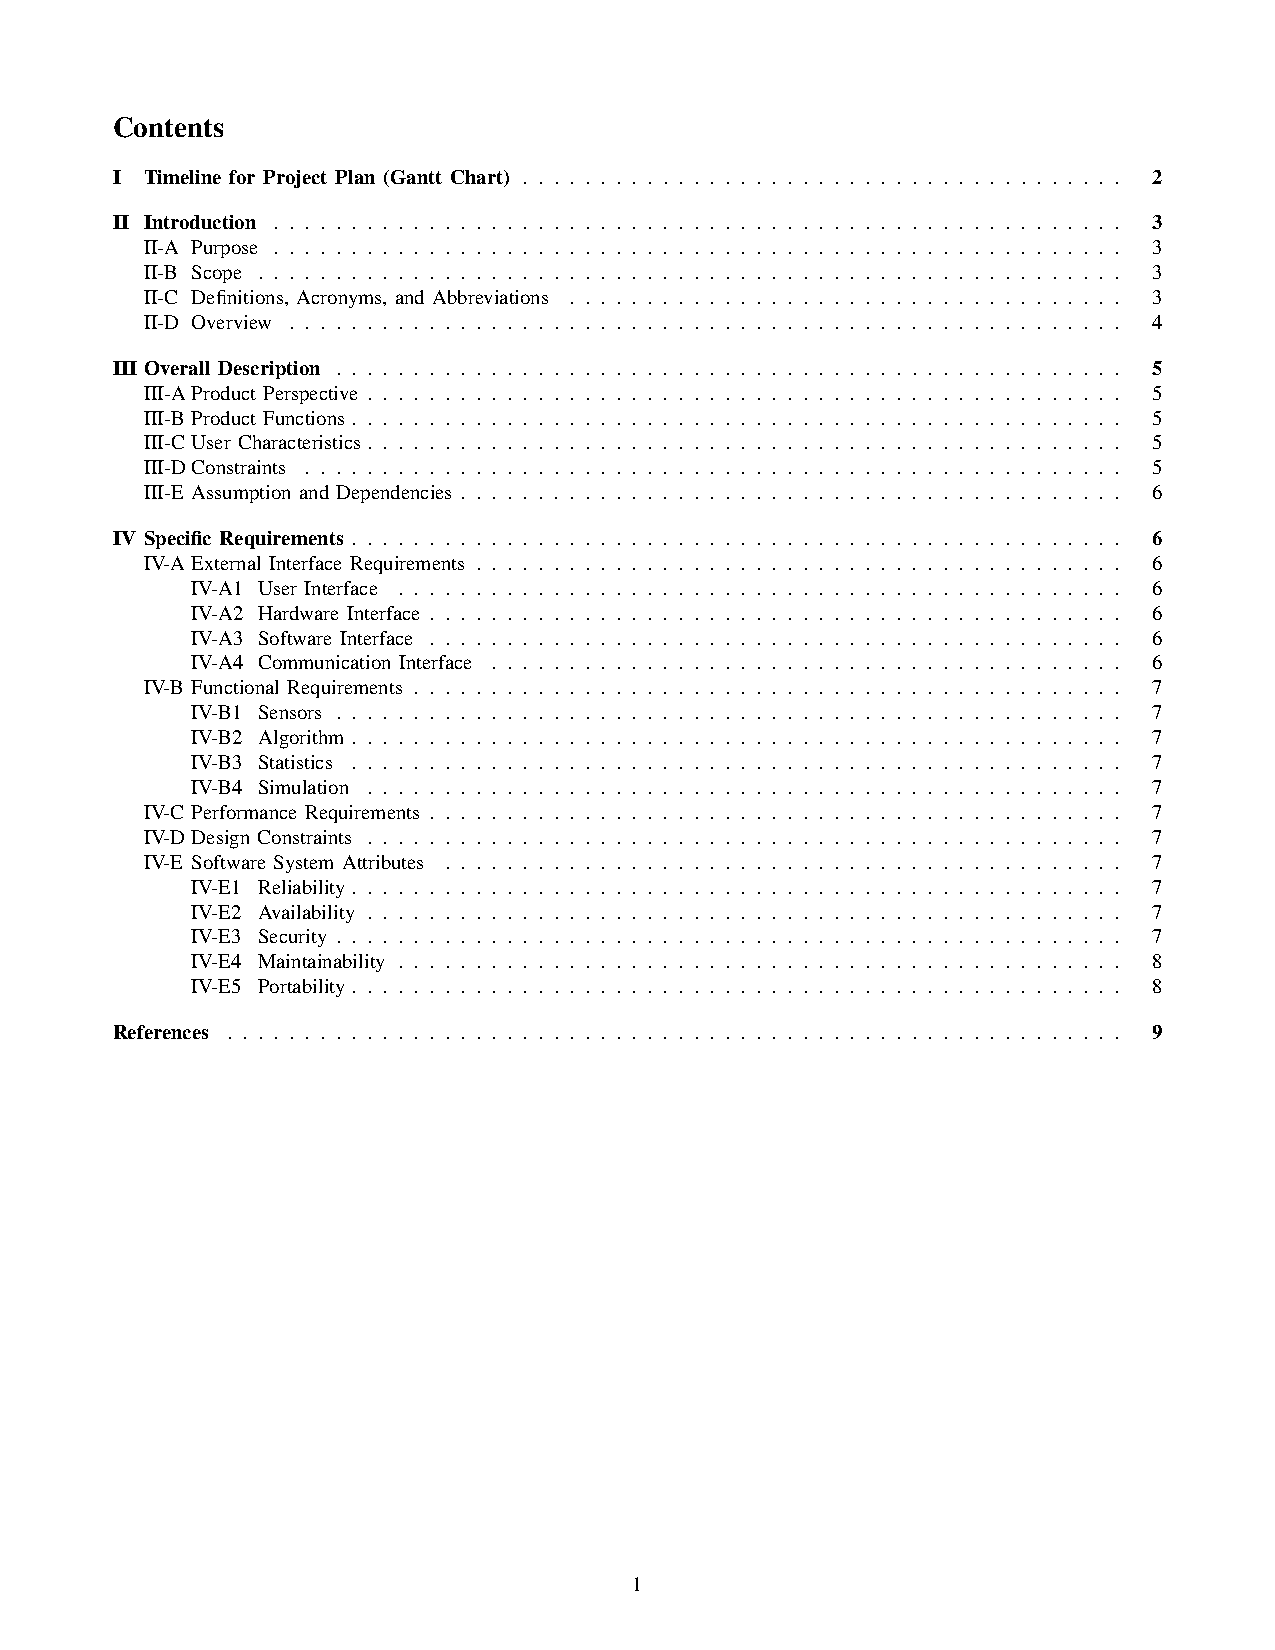
\includepdf[pages=-]{pdf/req_doc.pdf}

\newpage
\section{Change since Original Requirement Document}


\newpage
\section{Original Design Document}
\def\DDtitle{Computer Science Senior Software Engineering Project (CS462)}
\def\DDterm{Winter 2017}
	\begin{center}
		\vspace{\fill}

		{\Huge\bfseries Original Design Document\par}
		\vspace{0.5cm}
		{\Large\itshape \DDtitle\par}
		\vspace{0.5cm}
		{\Large\itshape \DDterm\par}
		
		\vspace{\fill}
	\end{center}
	\begin{abstract}
		A Head-up Display (HUD) Alignment system is developed as a proof of concept aims to explore a potential technological innovation for the HUD system that presents critical flight information to pilots. The primary objective of this project is to reduce the cost and time required to precisely align flight information to the HUD by introducing an additional sensor component to the system to make the alignment process more dynamic. This document is intended for use by Rockwell Collins and their HUD system development team. This document provides and explains an overall system framework, design viewpoints and specific design description for each viewpoint within the system.
	\end{abstract}
	
	\includepdf[pages=-]{pdf/design_doc.pdf}

\newpage
	\subsection{Necessary Change Based on Original Design}
		\subsubsection{Change in IV.COMSITION VIEW}
			\textbf{Hardware Configuration Design}
			\\ \indent The original diagram showed that the Aircraft IMU outputs aligned raw data to the microcontroller; what we did was both IMU would only output raw data and the alignment is measured/calculated by the microcontroller as figure~\ref{fig:hardware_config}.\\

			\begin{figure}
		 		\caption{New Data Flow diagram (Hardware)}
		      	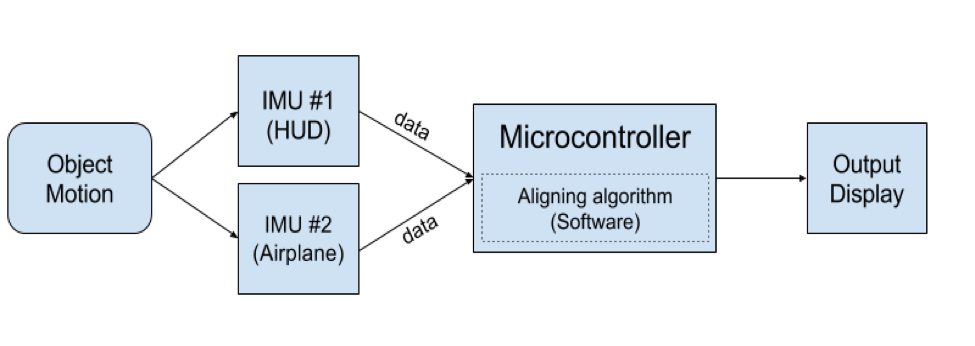
\includegraphics[width=\textwidth,height=\textheight,keepaspectratio]{hardware_config}
			    \label{fig:hardware_config}
			\end{figure}

		\subsubsection{Change In VI.INTERFACE VIEW}
			\textbf{Software User Interface Design}
			\\ \indent Our previous GUI have a 2D gauge-like looks to it. It looks more like a car dashboard rather than a real plane HUD. This GUI serve our purpose of showing the data well. However, it is hard to visualize the change on the plane for each angle. Our team is determined to give the best for this project and decided to improve on our GUI. To solve this problem, we create a new GUI as figure~\ref{fig:gui}  that visualize the change of angle to a plane object. We create this GUI by using a python sublanguage called VPython. We also use the pySerial library to connect the GUI to the Arduino part of the project.\\

			\begin{figure}
		 		\caption{New GUI by Vpython}
		      	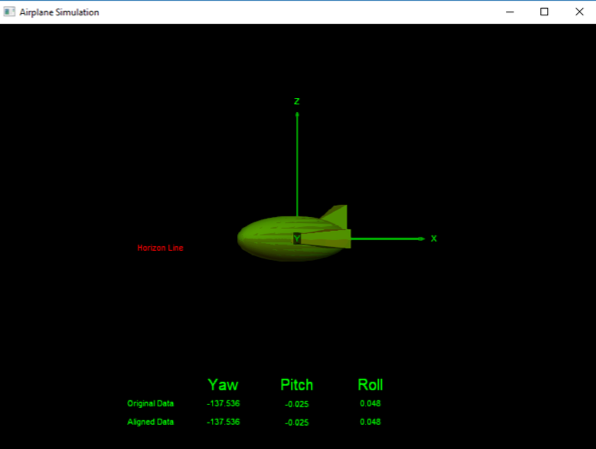
\includegraphics[width=\textwidth,height=\textheight,keepaspectratio]{gui}
			    \label{fig:gui}
			\end{figure}

		\subsubsection{Change In VIII Algorithm View}
			\textbf{Statistical Analysis Method for Initial Alignment Offset Design \& Offset Algorithm Design}
			\\ \indent For our statistical analysis, we applied a 95\% confidence interval to our offset data to ensure that the resulting offset was precise. By using a confidence interval, we can retrieve a valid offset value as soon as the quaternion value converges. Without using a confidence interval, we could end up with an erroneous value.

			Our implementation originally stored 60 samples each for the yaw, pitch and roll offset before using those values to find the confidence interval. Unfortunately, the microcontroller's memory is limited, which makes finding a precise value difficult. We were able to increase the number of samples and increase our performance by taking the offsets of each yaw, pitch and roll sequentially, thus tripling our sample sizes.

			Currently, the confidence interval is only being applied to the offsets between each device. Further improvements may be gained by increased use of statistical analysis. One such improvement would be to apply our analysis during calibration. The current process relies on a simple average of a single stream of data.













\newpage
\section{Original Tech Review}
\def\TRtitle{Computer Science Senior Software Engineering Project (CS462)}
\def\TRterm{Winter 2017}

	\begin{center}
		\vspace{\fill}

		{\Huge\bfseries Original Tech Review\par}
		\vspace{0.5cm}
		{\Large\itshape \TRtitle\par}
		\vspace{0.5cm}
		{\Large\itshape \TRterm\par}
		
		\vspace{\fill}
	\end{center}
	
	\begin{abstract}
		This project is a proof concept to explore a potential technological innovation for Head-Up Display (HUD) system that present critical flight information to pilots. The primary objective of this project is to reduce the cost and time required to precisely align flight information to the HUD by introducing additional sensor to the system to make the alignment process more dynamic. To achieve this goal, there are eight different main technologies that will be critical for the development of the project. This document will compare three alternative options for each main technologies. This document will also include the option that we choose for each main technologies to develop this project. 
	\end{abstract}
	
	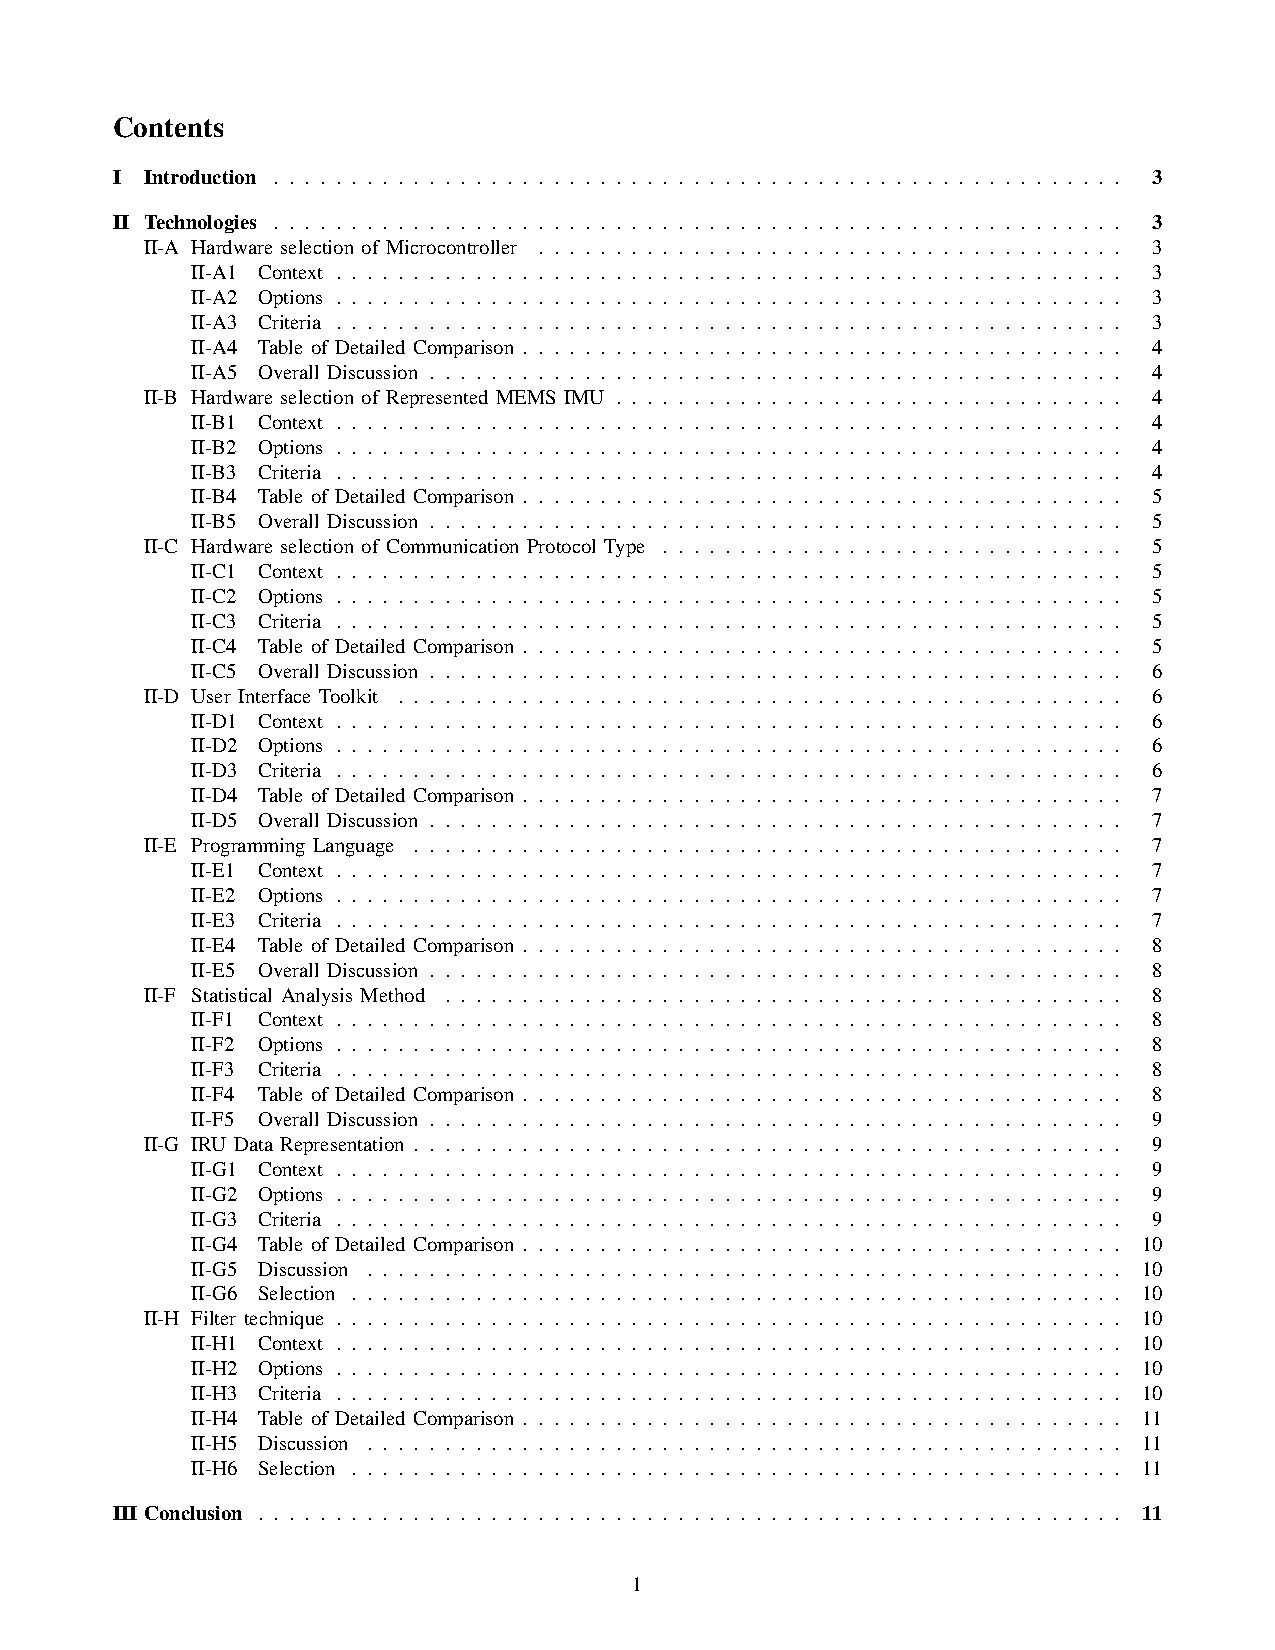
\includepdf[pages=-]{pdf/tech_review.pdf}

	\subsection{Necessary Change Based on Original Technology}
		\subsubsection{Change in D.User Interface Toolkit}
			Our previous GUI have a 2D gauge-like looks to it. It looks more like a car dashboard rather than a real plane HUD. This GUI serve our purpose of showing the data well. However, it is hard to visualize the change on the plane for each angle. Our team is determined to give the best for this project and decided to improve on our GUI. To solve this problem, we create a new GUI that visualize the change of angle to a plane object. We create this GUI by using a python library called VPython. We also use the pySerial library to connect the GUI to the Arduino part of the project, an new overall review seen as following:\\

			\begin{itemize}
				\item \textbf{Complexity:}
				least complex

				\item \textbf{Accessibility:}
				Free open source

				\item \textbf{Adoption Rate:}
				Few tutorials or examples

				\item \textbf{Time Commitment:}
				Minimal

				\item \textbf{Library:}
				Powerful
				
				\item \textbf{Overall Cost and Benefit:}
				Easy but powerful, but too few online tutorials could be found\\
			\end{itemize}

		\subsubsection{Change in F.Statistical Analysis Method}
			For our statistical analysis, we ended up applying a 95\% confidence interval to our offset data to ensure that the resulting offset was precise. Confidence interval is easier to be programmed but it also works well. In addition, by using a confidence interval, we can retrieve a valid offset value as soon as the quaternion value converges. Without using a confidence interval, we could end up with an erroneous value.













\newpage
\section{Weekly blog post}
	\subsection{Fall 2016}
%--------------------------------------------------------------------
%							Roger's Blog Post
%--------------------------------------------------------------------
		\subsubsection{Jiongcheng Luo (Fall 2016)}
		\vspace{0.5cm}

		\begin{center}
			\textbf{Week 3 (Oct. 10 {\textasciitilde{}} 14, 2016)}
		\end{center}
		\begin{itemize}
			\item \textbf{Plans for the coming week}
			\\My primary plan for next week is to complete the problem statement that is satisfied by the clients also have them sign on it. The next step is to understand the problem more in depth in the technical perspective, I hope to illustrate the problem by using mathematical and physics way, and be able to translate into CS problem such as what would be software program that we will build for the project.\\

			\item \textbf{Progress since last week}
			\\The most important progress I've made was I have built a better relationship with my teammates I have known them better. I also have a more clear understanding on the problem that we are trying to solve for the given project. We completed our first draft of problem statement even though it didn't meet the requirement from our clients, but it helped me comprehend the entire problem more deeply.\\

			\item \textbf{Any problems I encountered}
			\\It's hard to follow the agenda of our client, which we always had to wait for an uncertain long time for getting their email back, which may affect to our work progress in the future. In addition, the scheduling within our group is not settled yet, we have not yet set up a fixed time for the group meeting.\\
		\end{itemize}

		\rule{\textwidth}{0.5pt}

		\begin{center}
			\textbf{Week 4 (Oct. 16 {\textasciitilde{}} 21, 2016)}
		\end{center}
		\begin{itemize}
			\item \textbf{Plans for the coming week}
			\\By next week, the primary goal is to get the problem statement fixed as the expectation of the client, that in terms of the consistence of the entire statement. We will include more explanation in plain language to the technical terms. After that, I plan to do more and deeper researches, and start to working on the first design procedures to the problem.\\

			\item \textbf{Progress since last week}
			\\My progress is I understood how a team collaboration is so important to the success of this project, we have been getting closer as an entity and I started know the the character of each team member: what each of them good at and lack, that understanding helps me to know how to make better complement for each of us.\\

			\item \textbf{Any problems I encountered}
			\\The problem I met at this moment is how to improve the relationship between us and the client, since we had an issue that has led to breakdown of our relationship. Besides, I still have unclear problems for our projects such as the I am still not clear about the real time requirement for our algorithm, or like what kind of data we will get for test.\\
		\end{itemize}

		\rule{\textwidth}{0.5pt}

		\begin{center}
			\textbf{Week 5 (Oct. 23 {\textasciitilde{}} 28, 2016)}
		\end{center}
		\begin{itemize}
			\item \textbf{Plans for the coming week}
			\\The primary goal of next week is to complete the requirement document, which requires us to start thinking and planing for working on the project. I also plan to have one or two meetings with our client in regards to the requirement documents.\\

			\item \textbf{Progress since last week}
			\\My biggest progress from last week was that we have completed the problem statement as the expectation from our clients. And by that, I have become more familiar with the terminologies of our project, I have a clear picture in my mind about the problem that we are dealing with.\\

			\item \textbf{Any problems I encountered}
			\\I am still not sure about the resolution to our project, such as what kind of software and hardware we are going to play with. In other word, I am still not clear about our procedures for doing this project.\\
		\end{itemize}

		\rule{\textwidth}{0.5pt}

		\begin{center}
			\textbf{Week 6 (Oct. 31 {\textasciitilde{}} Nov. 5, 2016)}
		\end{center}
		\begin{itemize}
			\item \textbf{Plans for the coming week}
			\\By next week, I hope finish up the requirement document including all the sections/subsections; and I plan to decided which hardwares (boards) to use for our project and start thinking to purchase. And after decide which board to use, I plan to start looking at more detail of the board and maybe starting do some simple coding simulation.\\

			\item \textbf{Progress since last week}
			\\By writing on the requirement document, I know much better about the specific points of the project such as the detail workflow, input/output of the product and restriction, etc. In addition, we have known about what sort of boards that we are using for building the product, which helped me narrow the learning process so that I know what to look up and learn about.\\

			\item \textbf{Any problems I encountered}
			\\We are still struggling about some of the detail information about the product when writing on the requirement document, many specific points are unknown until we start the implementation.\\
		\end{itemize}

		\rule{\textwidth}{0.5pt}

		\begin{center}
			\textbf{Week 7 (Nov. 7 {\textasciitilde{}} Nov. 11, 2016)}
		\end{center}
		\begin{itemize}
			\item \textbf{Plans for the coming week}
			\\My plan for the next week is to finish up the the technology review, that's not only for the writing part, but also plan to list out and truly understand all the technologies that we may use as well as how to use these technologies for our project. Also, I plan to list out all the hardware that we are going to implement on and prepare to purchase for those.\\

			\item \textbf{Progress since last week}
			\\We have eventually finished the requirement document by last week and move on to the technologies review, by writing up the requirement document, I have a deeper understanding to the restriction and the problem that we may meet during the real implementation process.\\

			\item \textbf{Any problems I encountered}
			\\We still have no solutions or ideas for solving some of the specific problems. For example, we need two groups of input data and one of them represent the correct aligned "Aircraft" IRU data for this project, how do we get the "correct aligned" data, what reference do we take to assume those data we come up is correct?\\
		\end{itemize}

		\rule{\textwidth}{0.5pt}

		\begin{center}
			\textbf{Week 8 (Nov. 14 {\textasciitilde{}} Nov. 18, 2016)}
		\end{center}
		\begin{itemize}
			\item \textbf{Plans for the coming week}
			\\By this week, I plan to start up and hopefully finish a rough draft by the end of the week. I also nail down the all the hardware that we are going to use and send out the list to Kevin. In addition, I plan to send out an email to our client to report our progress and ask about some questions: 1. How to get correct aligned data as reference? 2. Ask for generic HUD symbology picture 3. GitHub Account.\\

			\item \textbf{Progress since last week}
			\\We have finished up our technologies review and we have discuss about the question about how to get correct aligned data as reference, even though we do not if our assumption will be correct or doable or not when doing the real implementation. But we assume we can "make" a group of correct aligned data by manually adjusting it and assume this data is correct, so that we will let the other group of data to be correctly aligned based on this assumption.\\

			\item \textbf{Any problems I encountered}
			\\The problem I had so far is for getting the correct aligned data as reference, and we have to figure out the hardware we going to use.\\
		\end{itemize}


%--------------------------------------------------------------------
%							Drew's Blog Post
%--------------------------------------------------------------------

		\subsubsection{Drew Hamm (Fall 2016)}
		\vspace{0.5cm}

		\begin{center}
			\textbf{Week 3 (Oct. 10 {\textasciitilde{}} 14, 2016)}
		\end{center}
		\begin{itemize}
			\item \textbf{Plans for the coming week}
			\\ I want to start looking into the hardware we might be working with for this project. Specifically I will be reading the specifications for both the Motion Sensor Evaluation Board: MPU-9250CA-SDK and the Ellipse-D: Miniature Dual GPS INS. Besides familiarizing myself with the hardware I want to learn about Quaternions as advised by our client in order to better understand the output data we will be working with. Lastly, I plan on finishing up my section of the problem statement as well as working with my team to finish it as a whole.\\

			\item \textbf{Progress since last week}
			\\Met up with team members to work on the problem statement and finish a first draft. Received feedback from clients further specifying the project details.\\

			\item \textbf{Any problems I encountered}
			\\I found out that my first understanding of the project was incorrect. At first I thought we were mostly working on a proof of concept. I realized my understanding of hardware error was poor. Since our project requires accurate results, I need to spend some time to understand how much error might be expected from our solution.\\
		\end{itemize}

		\rule{\textwidth}{0.5pt}

		\begin{center}
			\textbf{Week 4 (Oct. 17 {\textasciitilde{}} 21, 2016)}
		\end{center}
		\begin{itemize}
			\item \textbf{Plans for the coming week}
			\\ I'll be working together with the group in order to finish up a new revision of our problem statement. We want to address a couple of our clients concerns in order to get their signed approval. We have a meeting with our client on Wednesday to which I want to prepare questions for. We should also be able to get our problem statement signed so we can move on to working on the requirements document.\\

			\item \textbf{Progress since last week}
			\\Met with group to clear up some miscommunication we had with our client. Worked on on the problem statement along with research on both MEMS IRU and aircraft IRU specifications.\\

			\item \textbf{Any problems I encountered}
			\\The technical writing required to create the problem statement has been difficult. Most of this difficulty is due to having to learn the specialized terminology as well as hardware that we will be working with.\\
		\end{itemize}

		\rule{\textwidth}{0.5pt}

		\begin{center}
			\textbf{Week 5 (Oct. 24 {\textasciitilde{}} 28, 2016)}
		\end{center}
		\begin{itemize}
			\item \textbf{Plans for the coming week}
			\\ I will be working on the requirements document. This will also involve getting together with the group and doing more research in order to fully explain our solution. We will need to get in touch with our client once we have a working draft of the document.\\

			\item \textbf{Progress since last week}
			\\Finished our problem statement and met with our client. Our meeting was productive as it helped to answer a few questions we had as well as to ensure that we are covering everything of importance within our project.\\

			\item \textbf{Any problems I encountered}
			\\Schedule conflicts for myself and the group made this week difficult. Our solution was less meeting in person and more work being done online.\\
		\end{itemize}

		\newpage

		\begin{center}
			\textbf{Week 6 (Oct. 31 {\textasciitilde{}} Nov. 4, 2016)}
		\end{center}
		\begin{itemize}
			\item \textbf{Plans for the coming week}
			\\ Continue working on the requirements document. Hopefully finish by Friday. Send client our finished document.\\

			\item \textbf{Progress since last week}
			\\Met with group members and decided what sections we are each responsible for writing within the requirements document. Started writing the my sections of the document.\\

			\item \textbf{Any problems I encountered}
			\\Some aspects of the project are quite complex and will require extra time to research.\\
		\end{itemize}

		\rule{\textwidth}{0.5pt}

		\begin{center}
			\textbf{Week 7 (Nov. 7 {\textasciitilde{}} Nov. 11, 2016)}
		\end{center}
		\begin{itemize}
			\item \textbf{Plans for the coming week}
			\\ First, I need to decide what to include in the tech review. Next, the group needs to choose who will be responsible for each item. Lastly, start working on the tech review and finish it by Friday.\\

			\item \textbf{Progress since last week}
			\\We finished the requirements document and sent it off to our client.\\

			\item \textbf{Any problems I encountered}
			\\Last week was busy with midterms and other assignments. Both group members and myself struggled to find time to meet and finish the requirements document.\\
		\end{itemize}

		\rule{\textwidth}{0.5pt}

		\begin{center}
			\textbf{Week 8 (Nov. 14 {\textasciitilde{}} Nov. 18, 2016)}
		\end{center}
		\begin{itemize}
			\item \textbf{Plans for the coming week}
			\\ Although we submitted the tech review I want to look into our project for other options we might need to decide on later. Looking for additional items will carry over into starting work on the design document. Planning to meet with group so we can decide what sections everyone will be responsible for.\\

			\item \textbf{Progress since last week}
			\\Finished the tech review. Researched filter techniques for sensor data. Learned about advancements in MEMS quality assurance testing.\\

			\item \textbf{Any problems I encountered}
			\\We originally choose 9 items for the tech review however, one of the items was too straight forward to find alternative solutions. We had a hard time finding an additional item to include so we left the document with only 8. I found that the tech review took more time than expected to complete as the research I had to do was quite complicated.\\
		\end{itemize}

%--------------------------------------------------------------------
%							Krisna's Blog Post
%--------------------------------------------------------------------

		\subsubsection{Krisna Irawan (Fall 2016)}
		\vspace{0.5cm}

		\begin{center}
			\textbf{Week 3 (Oct. 10 {\textasciitilde{}} 14, 2016)}
		\end{center}
		\begin{itemize}
			\item \textbf{Plans for the coming week}
			\\I am planning to do more research on Quaternion, since we will be working on the data in terms of Quaternion rotation. I also want to finalize our problem statement and have a clear understanding of our project. Lastly, I want to start exploring the possibilities of solution that we comes up with. I tried to learn more about the correlation of the acceleration between two data and the error that the integration gives.\\

			\item \textbf{Progress since last week}
			\\My team and I work together on the problem statement this week. We also be able to get more information of this project from our clients and have a greater understanding of this project. We also have meetings that really challenge us to think more deeply about this project and make sure our team are on the same page. \\

			\item \textbf{Any problems I encountered}
			\\Although we have a better understanding than last week, it seems that we are still missing some of the points about this project. I am really grateful with the communication that our clients give to us, it is really help us to get a better understanding about this project. We also have difficulties in finding the perfect meeting time for our group. I am still not aware of my teammate’s schedule. However, we are successfully held our meeting this week and will improve on the schedule communication.\\
		\end{itemize}

		\rule{\textwidth}{0.5pt}

		\begin{center}
			\textbf{Week 4 (Oct. 17 {\textasciitilde{}} 21, 2016)}
		\end{center}
		\begin{itemize}
			\item \textbf{Plans for the coming week}
			\\I am planning to finalize our problem statement and get our final problem statement signed by our clients. I will also be working on the requirement documents and see if we have any more question about this project.\\

			\item \textbf{Progress since last week}
			\\My team and I work together on clearing the communication breakdown that happens this week between our team and our clients. I now have a clearer understanding on how to deal with a real work environment. \\

			\item \textbf{Any problems I encountered}
			\\We have a breakdown in our communication with our clients. We are trying to resolve this problem and got some tips from our teacher regarding this issues. This project going to be a learning curve for me, I have to learn more about some terminology and knowledge about hardware.\\
		\end{itemize}

		\rule{\textwidth}{0.5pt}

		\begin{center}
			\textbf{Week 5 (Oct. 24 {\textasciitilde{}} 28, 2016)}
		\end{center}
		\begin{itemize}
			\item \textbf{Plans for the coming week}
			\\I am planning to further refine our requirement documents and ask some clarification question to our clients (if any). We are also planning on getting our requirement document to be signed before the end of next week.\\

			\item \textbf{Progress since last week}
			\\We have another meetings with our clients this week on Wednesday. We clarify some stuff to move forward for our requirement documents. We also get our problem statement signed by our clients.\\

			\item \textbf{Any problems I encountered}
			\\ I have a time management problem when working on the requirement documents this week. My schedule for this week is packed with assignment and midterms. I haven't got an optimal time to do the requirement documents this week. However, I will refine our requirement documents during the weekend and hopefully can get feedback from our teacher before we send it to our clients.\\
		\end{itemize}

		\rule{\textwidth}{0.5pt}

		\begin{center}
			\textbf{Week 6 (Oct. 31 {\textasciitilde{}} Nov. 4, 2016)}
		\end{center}
		\begin{itemize}
			\item \textbf{Plans for the coming week}
			\\We will send our requirement documents to our client at the end of the week and see if we need to further refine our requirement document to be signed. I will also start to work on the Technical Review documents, looking for more options that we can do (or can't do) for this project.\\

			\item \textbf{Progress since last week}
			\\We work on the Requirement Document. Our clients has found out the ideal hardware that we will be working with for this project. Creating the requirement document makes me think more deeply about this project and how we going to achieve our goal. I got a clearer understanding on how to implements our project.\\

			\item \textbf{Any problems I encountered}
			\\The biggest problem for this week is time management. This week is a midterm week for all of us. This makes it hard for us to focus on the documents.\\
		\end{itemize}

		\rule{\textwidth}{0.5pt}

		\begin{center}
			\textbf{Week 7 (Nov. 7 {\textasciitilde{}} Nov. 11, 2016)}
		\end{center}
		\begin{itemize}
			\item \textbf{Plans for the coming week}
			\\ I will start investing my time in the Tech Review documents. I will ask more clarification question to the teacher about this documents. I will push myself in getting started with the design documents. \\

			\item \textbf{Progress since last week}
			\\We got a really good review for our requirement documents. Our clients are really pleased with the requirement documents that we send to them. I am glad that things works out and we pleased our clients with our work. \\

			\item \textbf{Any problems I encountered}
			\\The biggest problem that we faced is finding time to meet together and spend our time working together on the documents. We also have some question about our project during the weeks but our clients clarify those stuff and really help us to get the information that we need.\\
		\end{itemize}

		\rule{\textwidth}{0.5pt}

		\begin{center}
			\textbf{Week 8 (Nov. 14 {\textasciitilde{}} Nov. 18, 2016)}
		\end{center}
		\begin{itemize}
			\item \textbf{Plans for the coming week}
			\\ We are trying our best to finish our Design Documents before the thanks giving break. \\

			\item \textbf{Progress since last week}
			\\We already submitted our signed requirement documents on Monday. We have finished our Tech review documents on Wednesday noon. \\

			\item \textbf{Any problems I encountered}
			\\Working on the Tech Review documents makes me think more deeply about the project and how we actually going to build this project. This requires me to do a lot of research and make a design decision.\\
		\end{itemize}

		\rule{\textwidth}{0.5pt}

		\begin{center}
			\textbf{Week 9 (Nov. 21 {\textasciitilde{}} Nov. 25, 2016)}
		\end{center}
		\begin{itemize}
			\item \textbf{Plans for the coming week}
			\\ We will be working on the Design documents and finished it before Wednesday. We will be working on the Progress report after we submit the design documents to the clients. \\

			\item \textbf{Progress since last week}
			\\ We get the foundation for the design documents ready. We have a better idea about the progress report. \\

			\item \textbf{Any problems I encountered}
			\\It was hard to find a time to work on the document during thanks giving break.\\
		\end{itemize}

		\rule{\textwidth}{0.5pt}

		\begin{center}
			\textbf{Week 10 (Nov. 28 {\textasciitilde{}} Dec. 2, 2016)}
		\end{center}
		\begin{itemize}
			\item \textbf{Plans for the coming week}
			\\Finished up the progress report document and video. \\

			\item \textbf{Progress since last week}
			\\We get the design document submitted. \\

			\item \textbf{Any problems I encountered}
			\\Busy schedule for dead week.\\
		\end{itemize}









\newpage
	\section{Winter 2016}

%--------------------------------------------------------------------
%							Roger's Blog Post
%--------------------------------------------------------------------
	\subsection{Jiongcheng Luo (Winter 2016)}
	\vspace{0.5cm}

	\begin{center}
		\textbf{Week 1 (Jan. 9 {\textasciitilde{}} 13, 2017)}
	\end{center}
	\begin{itemize}
		\item \textbf{Plans for the coming week}
		\\Getting all the basic hardware components and devices, start working on hardware setup including board hoop-up and sample code testing. Also set up a meeting with our clients to talk about plans and changes of the project progress.\\

		\item \textbf{Progress since last week}
		\\We held the first group meeting of the term and we decided to purchase our own board if the hardware not arriving yet.\\

		\item \textbf{Any problems I encountered}
		\\Delayed on getting the necessary hardware components and we couldn't start the implementation.\\
	\end{itemize}

	\rule{\textwidth}{0.5pt}

		
	\begin{center}
		\textbf{Week 2 (Jan. 16 {\textasciitilde{}} 20, 2017)}
	\end{center}
	\begin{itemize}
		\item \textbf{Plans for the coming week}
		\\Getting all the basic hardware components and devices ASAP, start working on hardware setup including board hoop-up and sample code testing, modify the project schedule that due that to the delayed hardware devices\\

		\item \textbf{Progress since last week}
		\\We held the first meeting with the client and talked about our plan and blocks currently.\\

		\item \textbf{Any problems I encountered}
		\\Still have not yet gotten the necessary hardware components and we couldn't start the implementation.\\
	\end{itemize}


\newpage
%--------------------------------------------------------------------
%							Drew's Blog Post
%--------------------------------------------------------------------
	\subsection{Drew Hamm (Winter 2016)}
	\vspace{0.5cm}
	Miss.

%--------------------------------------------------------------------
%							Krisna's Blog Post
%--------------------------------------------------------------------
	\subsection{Krisna Irawan (Winter 2016)}
	\vspace{0.5cm}

	\begin{center}
		\textbf{Week 1 (Jan. 9 {\textasciitilde{}} 13, 2017)}
	\end{center}
	\begin{itemize}
		\item \textbf{Plans for the coming week}
		\\We will tried to get all the necessary hardware to start this project. We will have a meeting with our clients on Wednesday next week. \\

		\item \textbf{Progress since last week}
		\\We meet as a group this week. We have a solid plan for next week. \\

		\item \textbf{Any problems I encountered}
		\\Getting started with all the logistic and the scheduling of the class and the project. Trying to get all the necessary hardware for this project.\\
	\end{itemize}

	\rule{\textwidth}{0.5pt}

	\begin{center}
		\textbf{Week 2 (Jan. 16 {\textasciitilde{}} 20, 2017)}
	\end{center}
	\begin{itemize}
		\item \textbf{Plans for the coming week}
		\\We will tried to get all the necessary hardware to start this project. We are trying our best to meet with our teacher to get the hardware. \\

		\item \textbf{Progress since last week}
		\\We meet as a group with our clients last Wednesday. We let them know about our logistic problem. \\

		\item \textbf{Any problems I encountered}
		\\Getting started with all the logistic and the scheduling of the class and the project. Trying to get all the necessary hardware for this project.\\
	\end{itemize}

	\rule{\textwidth}{0.5pt}

	\begin{center}
		\textbf{Week 3 (Jan. 23 {\textasciitilde{}} 27, 2017)}
	\end{center}
	\begin{itemize}
		\item \textbf{Plans for the coming week}
		\\We will start on the implementation of the project. We will finished up the hardware set up and a brief user interface. \\

		\item \textbf{Progress since last week}
		\\We finally get our hardware last Thursday. We can now really start on the implementation of the project. \\

		\item \textbf{Any problems I encountered}
		\\The logistic problem really set us back for a couple week behind the schedule. We will work hard to catch up with that.\\
	\end{itemize}

	\rule{\textwidth}{0.5pt}

	\begin{center}
		\textbf{Week 4 (Jan. 30 {\textasciitilde{}} Feb. 3, 2017)}
	\end{center}
	\begin{itemize}
		\item \textbf{Plans for the coming week}
		\\Continue to develop the user interface. \\

		\item \textbf{Progress since last week}
		\\We have a brief user interface. \\

		\item \textbf{Any problems I encountered}
		\\Getting the hardware setup.\\
	\end{itemize}

	\rule{\textwidth}{0.5pt}

	\begin{center}
		\textbf{Week 5 (Feb. 6 {\textasciitilde{}} Feb. 10, 2017)}
	\end{center}
	\begin{itemize}
		\item \textbf{Plans for the coming week}
		\\Finished up the midterm progress report and document revisions. \\

		\item \textbf{Progress since last week}
		\\Our user interface is ready and finished. \\

		\item \textbf{Any problems I encountered}
		\\There is no generic user interface plug-in that I can use. I have to create the user interface from scratch.\\
	\end{itemize}

	\rule{\textwidth}{0.5pt}

	\begin{center}
		\textbf{Week 5 (Feb. 6 {\textasciitilde{}} Feb. 10, 2017)}
	\end{center}
	\begin{itemize}
		\item \textbf{Plans for the coming week}
		\\Continue with the User Interface first user study. \\

		\item \textbf{Progress since last week}
		\\We finished the midterm progress report and revision for our documents. \\

		\item \textbf{Any problems I encountered}
		\\Finishing up the documents and video took most of our time this week.\\
	\end{itemize}

	\rule{\textwidth}{0.5pt}

	\begin{center}
		\textbf{Week 6 (Feb. 13 {\textasciitilde{}} Feb. 17, 2017)}
	\end{center}
	\begin{itemize}
		\item \textbf{Plans for the coming week}
		\\Continue with the User Interface first user study. \\

		\item \textbf{Progress since last week}
		\\We finished the midterm progress report and revision for our documents. \\

		\item \textbf{Any problems I encountered}
		\\Finishing up the documents and video took most of our time this week.\\
	\end{itemize}

	\rule{\textwidth}{0.5pt}

	\begin{center}
		\textbf{Week 7 (Feb. 13 {\textasciitilde{}} Feb. 17, 2017)}
	\end{center}
	\begin{itemize}
		\item \textbf{Plans for the coming week}
		\\Start to work on the statistical analysis portion of this project. \\

		\item \textbf{Progress since last week}
		\\We finished the midterm progress report and revision for our documents. \\

		\item \textbf{Any problems I encountered}
		\\We do not have a chance to meet this week.\\
	\end{itemize}

	\rule{\textwidth}{0.5pt}

	\begin{center}
		\textbf{Week 8 (Feb. 27 {\textasciitilde{}} Mar. 3, 2017)}
	\end{center}
	\begin{itemize}
		\item \textbf{Plans for the coming week}
		\\Start to work on the statistical analysis portion of this project. \\

		\item \textbf{Progress since last week}
		\\Continue to work on the statistical analysis portion of this project. \\

		\item \textbf{Any problems I encountered}
		\\We do not know the structure of this class. We are not sure where we at in the class in terms of grades.\\
	\end{itemize}

	\rule{\textwidth}{0.5pt}

	\begin{center}
		\textbf{Week 9 (Mar. 3 {\textasciitilde{}} Mar. 10, 2017)}
	\end{center}
	\begin{itemize}
		\item \textbf{Plans for the coming week}
		\\Work on the poster. \\

		\item \textbf{Progress since last week}
		\\We have a class meeting this week. We were practicing for the expo \\

		\item \textbf{Any problems I encountered}
		\\We have to finished up the project soon.\\
	\end{itemize}

	\rule{\textwidth}{0.5pt}

	\begin{center}
		\textbf{Week 10 (Mar. 13 {\textasciitilde{}} Mar. 17, 2017)}
	\end{center}
	\begin{itemize}
		\item \textbf{Plans for the coming week}
		\\Finished up the progress report. Connect the user interface and statistical analysis to the Arduino module \\

		\item \textbf{Progress since last week}
		\\We finished the poster \\

		\item \textbf{Any problems I encountered}
		\\We have to finished up the progress report during finals week.\\
	\end{itemize}












\newpage
	\subsection{Spring 2016}

%--------------------------------------------------------------------
%							Roger's Blog Post
%--------------------------------------------------------------------
	\subsubsection{Jiongcheng Luo (Spring 2016)}
	\vspace{0.5cm}

	\begin{center}
		\textbf{Week 1 (Apr. 3 {\textasciitilde{}} 7, 2017)}
	\end{center}
	\begin{itemize}
		\item \textbf{Plans for the coming week}
		\\As the first week after break, I plan to have a meeting with the entire group as well as our clients, we will plan to give a short report to them and we plan to move on with our project\\

		\item \textbf{Progress since last week}
		\\I briefly took a look at the new schedule of the spring term and start making plan based on our current situation.\\

		\item \textbf{Any problems I encountered}
		\\We still found hard to retrieve two sets of data from the two different IMUs, we considered our old GUI program is NOT clearly enough to for our demonstration purpose, we planned to develop a new GUI program.\\
	\end{itemize}

	\rule{\textwidth}{0.5pt}

	\begin{center}
		\textbf{Week 2 (Apr. 10 {\textasciitilde{}} 14, 2017)}
	\end{center}
	\begin{itemize}
		\item \textbf{Plans for the coming week}
		\\By the coming week, we plan to update and fix our poster as the second draft. We also plan to group up to work on the project together, specifically will focus on the design of the UI of the demonstration system.\\

		\item \textbf{Progress since last week}
		\\We held our first meeting since the spring break and we planned out our schedule for the rest of the term.\\

		\item \textbf{Any problems I encountered}
		\\We found hard to fix the poster since everything is on a very level terminology, and since we have not done the statical analysis for our final testing result, we won't be able to put a specific result onto the poster.\\
	\end{itemize}

	\rule{\textwidth}{0.5pt}

	\begin{center}
		\textbf{Week 3 (Apr. 17 {\textasciitilde{}} 21, 2017)}
	\end{center}
	\begin{itemize}
		\item \textbf{Plans for the coming week}
		\\We plan to fix our poster for the final draft and have it send to our client for verification. We also plan to meet up again to continue woking on the project together.\\

		\item \textbf{Progress since last week}
		\\We got some feedback from the TA in terms of how to fix and update for our poster. We finally found a Python library called VPython that is easy to implement, and it provides ideal graphical interface (3D model animation) for our project virtual demonstration, we have also figured out the hardware configuration in terms of getting data from two IMUs as different addresses.\\

		\item \textbf{Any problems I encountered}
		\\We could not illustrate the best graphical display model for showing off to the audience in the expo, we want it to be straight forward and understandable, but also be able to demonstrate our result and outcome of the complex system.\\
	\end{itemize}

	\rule{\textwidth}{0.5pt}

	\begin{center}
		\textbf{Week 4 (Apr. 24 {\textasciitilde{}} 28, 2017)}
	\end{center}
	\begin{itemize}
		\item \textbf{Plans for the coming week}
		\\We will try to finish up everything for the project and have a well plan for the demonstration in the expo. We had grouped up again and made some progress on the project.\\

		\item \textbf{Progress since last week}
		\\We fixed the refined our poster, we submitted the final draft of poster to our client, everything looks good to them.\\

		\item \textbf{Any problems I encountered}
		\\We could not show our result to our client as they expect, we are still trying to improve the accuracy and stability of our output, and we will figure out the best way to show off the detail of the alignment.\\
	\end{itemize}

	\rule{\textwidth}{0.5pt}

	\begin{center}
		\textbf{Week 5 (May. 1 {\textasciitilde{}} 5, 2017)}
	\end{center}
	\begin{itemize}
		\item \textbf{Plans for the coming week}
		\\We will try to finish up putting the Arduino program with the demonstration UI program together and test for expo demonstration, we will make a detailed plan for the demonstration in the expo, also plan to show our result to our client see if we can improve based on what we have.\\

		\item \textbf{Progress since last week}
		\\We finally submitted our poster for printing. We roughly finished all implementation on the software part of the project, and we updated our github repo with the latest version of our project, and we also updated the README file in terms of our project description.\\

		\item \textbf{Any problems I encountered}
		\\We could not improve the accuracy for the final output result, we may need to ask for some suggestions from our client, we also have not not yet test for the performance of the GUI, we may need to spend some time to debug.\\
	\end{itemize}

	\rule{\textwidth}{0.5pt}

	\begin{center}
		\textbf{Week 6 (May. 8 {\textasciitilde{}} 12, 2017)}
	\end{center}
	\begin{itemize}
		\item \textbf{Plans for the coming week}
		\\The Friday of coming week will be the engineering EXPO day, so we plan to finalize our project for the expo demonstration, and we also plan to build our demonstration system.\\

		\item \textbf{Progress since last week}
		\\We have finalized our GUI and we found out that our dynamic alignment process makes a not bad result.\\

		\item \textbf{Any problems I encountered}
		\\We found out a our result is not accurate enough especially and we believe that is because of something goes wrong with yaw calculation or implementation, but we could not determine if the problem comes from the hardware or our algorithm.\\
	\end{itemize}

	\rule{\textwidth}{0.5pt}

	\begin{center}
		\textbf{Week 7 (May. 15 {\textasciitilde{}} 19, 2017)}
	\end{center}
	\begin{itemize}
		\item \textbf{Plans for the coming week}
		\\We plan to implement our physical test on our current system and we also plan to set up a meeting with our client to report our result.\\

		\item \textbf{Progress since last week}
		\\We finally held our EXPO last week, although we could not complete our project in hundred percent, we did demonstrated our project and we did attracted a number of visitors to our expo. And even though our project seems to be hard to understand for general audience, some people were still quite interested in knowing about our project.\\

		\item \textbf{Any problems I encountered}
		\\We could not demonstrate our system with the static alignment algorithm since something goes wrong within the algorithm. Another problem I encountered was that I could not explain my project clearly to the audiences, I could not explain well to those who do not have any background knowledge about our project.\\
	\end{itemize}

	\rule{\textwidth}{0.5pt}

	\begin{center}
		\textbf{Week 8 (May. 22 {\textasciitilde{}} 26, 2017)}
	\end{center}
	\begin{itemize}
		\item \textbf{Plans for the coming week}
		\\We plan to do our final physical test to verify our result and also plan to set up a meeting with our client to report our final progress.\\

		\item \textbf{Progress since last week}
		\\We discussed and designed for the physical test.\\

		\item \textbf{Any problems I encountered}
		\\We did not set up the meeting with our client yet since we have not finished the physical test.\\

		\item \textbf{If you were to redo the project from Fall term, what would you tell yourself?}
		\\You should start working on the project as soon as possible discussed with the client mote often.\\

		\item \textbf{What is the biggest skill you've learned?}
		\\The biggest skill I learned is how to get into a field that I am unfamiliar with before or even not having any experience, my project is kind of like that, which I did not know anything about my project or any background knowledge before I really worked on it, however, throughout this project, I learned how to get start with a project like this.\\

		\item \textbf{What skills do you see yourself using in the future?}
		\\I think I will use the skill of dealing with projects involve in both hardware and software.\\

		\item \textbf{What did you like about the project, and what did you not?}
		\\I like that my project was not purely dealing with software or programming, but involve much with hardware, physics and mathematics; One thing I do not like about my project is that we did not have much resources or equipments to test with, we got only some conceptual ideas and thoughts and we did not have the chance to work with the real HUD (equipment).\\

		\item \textbf{What did you learn from your teammates?}
		\\From Drew, I learned that we should not rely on other external examples or existed libraries too much during implementing our project, we should design our own one based on other resources.\\

		\item \textbf{If you were the client for this project, would you be satisfied with the work done?}
		\\ I probably will not be 100\% satisfied with the current work done since we did not have a result as expected, however I can understand with that since we had limited time, knowledge and resources for our project implementation.\\

		\item \textbf{If your project were to be continued next year, what do you think needs to be working on?}
		\\First we can test with varied models of IMUs and select the one that has the best performance and is the easiest to deal with, then we will try to use more IMUs to work together for achieving better performance, and the most important thing that I consider need to be worked on is to design a complete test procedures for in order to precisely test the output of the system.\\
	\end{itemize}


%--------------------------------------------------------------------
%							Drew's Blog Post
%--------------------------------------------------------------------
\newpage
	\subsubsection{Drew Hamm (Spring 2016)}
	\vspace{0.5cm}

	\begin{center}
		\textbf{Week 1 (Apr. 3 {\textasciitilde{}} 7, 2017)}
	\end{center}
	\begin{itemize}
		\item \textbf{Plans for the coming week}
		\\Meet with our group and work on the micro controller code as well as the GUI.\\

		\item \textbf{Progress since last week}

		\item \textbf{Any problems I encountered}
		\\ I've been looking for a new place to live and finally moved this week so so my time has been limited.\\
	\end{itemize}

	\rule{\textwidth}{0.5pt}

	\begin{center}
		\textbf{Week 2 (Apr. 10 {\textasciitilde{}} 14, 2017)}
	\end{center}
	\begin{itemize}
		\item \textbf{Plans for the coming week}
		\\I am planning to work on the poster for expo as well as further improving our code.\\

		\item \textbf{Progress since last week}
		\\I met with our group over the weekend to discuss the project and make plans for the term.\\

		\item \textbf{Any problems I encountered}
		\\We are using a I2C bus to facilitate communication between devices in our project. However, their is a limit to the length in which the I2C bus may be before negatively effecting its performance. This may be a problem given the realized interconnectivity within an aircraft.\\
	\end{itemize}

	\rule{\textwidth}{0.5pt}

	\begin{center}
		\textbf{Week 3 (Apr. 17 {\textasciitilde{}} 21, 2017)}
	\end{center}
	\begin{itemize}
		\item \textbf{Plans for the coming week}
		\\I continue making improvements to our code in terms of refactoring. I will work on improving the calibration and static alignment processes.\\

		\item \textbf{Progress since last week}
		\\I made changes to our poster to improve readability as well as adding the necessary content required by my part. I started refactoring our code to improve readability as well as to promote further development.\\

		\item \textbf{Any problems I encountered}
		\\The magnetometer data seems to be skewed. We are having trouble deciding on the data and format to be sent to the GUI.\\
	\end{itemize}

	\rule{\textwidth}{0.5pt}

	\begin{center}
		\textbf{Week 4 (Apr. 24 {\textasciitilde{}} 28, 2017)}
	\end{center}
	\begin{itemize}
		\item \textbf{Plans for the coming week}
		\\ Improve the calibration process and submit the final version of our project in terms of what will be graded. I need to submit my release form for expo.\\

		\item \textbf{Progress since last week}
		\\I met with our group to continue work on our solution and test it with the GUI. I made changes to our poster to improve grammar and adjust positioning of elements. We finished and submitted our poster\\

		\item \textbf{Any problems I encountered}
		\\Inconsistent calibration results and limited micro controller memory. Started using the Arduino IDE serial plotter for analyzing individual sensor data which has been insightful. We also need to perform physical tests on our system but we are having a hard time creating a plan of attack.\\
	\end{itemize}

	\rule{\textwidth}{0.5pt}

	\begin{center}
		\textbf{Week 5 (May. 1 {\textasciitilde{}} 5, 2017)}
	\end{center}
	\begin{itemize}
		\item \textbf{Plans for the coming week}
		\\Research methods for improving data readings and sample selection. Work on the midterm progress report. We will be meeting with another team to review each others posters and give feedback.\\

		\item \textbf{Progress since last week}
		\\I was able to push a working version of our alignment solution. Submitted my release form for expo.\\

		\item \textbf{Any problems I encountered}
		\\When taking the offset using quaternions I found that the result was inaccurate while the quaternion was converging as a result of the filter algorithm. I tried to remove samples taken during the convergence period by analyzing the change of values over time. More work needs to be done to improve this process. Another problem I faced had to do with the error of individual samples. Even when the device was stationary, I noticed values spiking at times. I attempted to remove these samples by using a hard coded threshold that was determined heuristically. I'm not sure what the best approach would be at this current time.\\
	\end{itemize}

	\rule{\textwidth}{0.5pt}

	\begin{center}
		\textbf{Week 6 (May. 8 {\textasciitilde{}} 12, 2017)}
	\end{center}
	\begin{itemize}
		\item \textbf{Plans for the coming week}
		\\We will meeting up to make some last minute changes with our project in terms of what will be displayed during expo.\\

		\item \textbf{Progress since last week}
		\\We have been having problems with the magnetometer data and poor readings. I'm not sure if I miss configured the device or am not performing sufficient calibration. Since expo is next week, we will explore a 6-axis filter instead of the 9-axis filter.\\

		\item \textbf{Any problems I encountered}
		\\Worked with Krisna to add the statistical confidence interval when finding the static offset. Our group met with another group to review each others posters and provide feedback. We started working on our midterm progress report.\\
	\end{itemize}

	\rule{\textwidth}{0.5pt}

	\begin{center}
		\textbf{Week 7 (May. 15 {\textasciitilde{}} 19, 2017)}
	\end{center}
	\begin{itemize}
		\item \textbf{Plans for the coming week}
		\\We will try to make plans to test our system.\\

		\item \textbf{Progress since last week}
		\\I finished my part of the midterm progress report. We met up to discuss our project to ensure we were all on the same page for expo. We built a simple demonstration system that could be manipulated during expo to help explain our project. EXPO!\\

		\item \textbf{Any problems I encountered}
		\\My audio input is not working so I had to meet up with Roger and use his laptop to record my presentation. Our system has yet to undergo the physical tests that are required before sending our results to RC. Since our system has yet to be tested, I realized late that our solution was not correctly checking for static offset. In order to make our solution work, we would have to move the HUD sensor from the IRU to the HUD and then take the difference. Our error was a result of testing our system on a with an aligned axis. What we were really detection was simple the sensor bias. Our false interpretation was reaffirmed because we were successfully taking the dynamic offset.\\
	\end{itemize}

	\rule{\textwidth}{0.5pt}

	\begin{center}
		\textbf{Week 8 (May. 22 {\textasciitilde{}} 26, 2017)}
	\end{center}
	\begin{itemize}
		\item \textbf{Plans for the coming week}
		\\I am planning on meeting with our group and getting in contact with our client. I'm also planning on working on our final documents.\\

		\item \textbf{Progress since last week}
		\\Started working on our final documents.\\

		\item \textbf{Any problems I encountered}
		\\We were not able to meet this week so testing the system and contacting our client delayed.\\

		\item \textbf{If you were to redo the project from Fall term, what would you tell yourself?}
		\\First of all, I would tell myself to setup version control early and make use of the skills learned in my software development classes to promote collaboration and a sense of direction while building momentum as milestones were reached. Next, I would tell myself to utilize the availability of our clients by asking more questions when referencing the technical challenges of our project. Lastly, I would stress testing early; both physically and programmatically.\\

		\item \textbf{What is the biggest skill you've learned?}
		\\ I think biggest skill I have learned would have to be the ability to work with sensors such as an accelerometer, gyroscope and magnetometer. I choose this because there was a lot involved. First, I had to learn how to configure devices by reading through the devices register mapping documentation. Next, I had to learn how to calibrate the devices by taking initial readings during setup, comparing them against factory defaults and storing the results in the appropriate registers or using that information to modify future readings. I also had to learn how communication between devices worked and why and how some devices should be configure as slaves or masters.\\

		\item \textbf{What skills do you see yourself using in the future?}
		\\Considering the shift towards the Internet of things, I can see myself working with multiple devices while facilitating the necessary communication for those devices in future work or even hobby projects.\\

		\item \textbf{What did you like about the project, and what did you not?}
		\\I liked that I was given an opportunity to work in an area I was not familiar with. I did not like how much work was required to catch up in understanding of particular topics when I would have rather been making significant progress towards a solution.\\

		\item \textbf{What did you learn from your teammates?}
		\\I learned additional interpersonal skills and strategies to overcome poor first impressions. My team also helped me to learn skills relating to latex and vpython.\\

		\item \textbf{If you were the client for this project, would you be satisfied with the work done?}
		\\ I would have liked to see a better solution but I believe the documented requirements have been met.\\

		\item \textbf{If your project were to be continued next year, what do you think needs to be working on?}
		\\Memory considerations when analyzing sensor output. Improve calibration of sensors then test against documented hardware error tolerance specifications. Magnetometer considerations. Physical tests against filtered quaternion output and the resulting offset with static values. Look into physically testing dynamic values. Research methods to handle drift such as resetting to a known reference then finding ways to physically test against under expected conditions.\\
	\end{itemize}

%--------------------------------------------------------------------
%							Krisna's Blog Post
%--------------------------------------------------------------------
\newpage
	\subsubsection{Krisna Irawan (Spring 2016)}
	\vspace{0.5cm}

	\begin{center}
		\textbf{Week 1 (Apr. 3 {\textasciitilde{}} 7, 2017)}
	\end{center}
	\begin{itemize}
		\item \textbf{Plans for the coming week}
		\\We are planning to set up a meeting with our clients. We are planning to work together on our project this weekend. Hopefully we can finished up our project before week 3. \\

		\item \textbf{Progress since last week}
		\\We know the schedule for the class this term. We know our plan for this term. \\

		\item \textbf{Any problems I encountered}
		\\ To connect the statistical analysis portion, I need the data from the offset algorithm. Our team still working on the offset algorithm.\\
	\end{itemize}

	\rule{\textwidth}{0.5pt}

	\begin{center}
		\textbf{Week 2 (Apr. 10 {\textasciitilde{}} 14, 2017)}
	\end{center}
	\begin{itemize}
		\item \textbf{Plans for the coming week}
		\\We are planning to finished up the poster. We also planning to meet up with other groups to do the extra credit for this class. \\

		\item \textbf{Progress since last week}
		\\We meet with the TA and talk about our current state and where we are heading next. \\

		\item \textbf{Any problems I encountered}
		\\We are not able to do much work this week.\\
	\end{itemize}

	\rule{\textwidth}{0.5pt}

	\begin{center}
		\textbf{Week 3 (Apr. 17 {\textasciitilde{}} 21, 2017)}
	\end{center}
	\begin{itemize}
		\item \textbf{Plans for the coming week}
		\\We are planning to finished up the project this week. We are hoping to get the poster signed by our clients this week. \\

		\item \textbf{Progress since last week}
		\\We the poster feedback from our TA, we will incorporate that feedback to our poster. We are almost done with the project. We take care of the algorithm and reading from 2 sensors. \\

		\item \textbf{Any problems I encountered}
		\\ We found a language called vpython that will help us to create the 3d simulation of the HUD. We are still learning about this language.\\
	\end{itemize}

	\rule{\textwidth}{0.5pt}

	\begin{center}
		\textbf{Week 4 (Apr. 24 {\textasciitilde{}} 28, 2017)}
	\end{center}
	\begin{itemize}
		\item \textbf{Plans for the coming week}
		\\Set up an interview for the WIRED style review. Finished up the WIRED style review. \\

		\item \textbf{Progress since last week}
		\\I finished making the 3d simulation and convert the statistical analysis portion to python. \\

		\item \textbf{Any problems I encountered}
		\\We have to wrap up our project before the code freeze on May 1st. We will be working hard this weekend.\\
	\end{itemize}

	\rule{\textwidth}{0.5pt}

	\begin{center}
		\textbf{Week 5 (May. 1 {\textasciitilde{}} 5, 2017)}
	\end{center}
	\begin{itemize}
		\item \textbf{Plans for the coming week}
		\\Start to work on the midterm progress report. Finishing the hardware user interface setup.\\

		\item \textbf{Progress since last week}
		\\I finished the WIRED style review assignment. \\

		\item \textbf{Any problems I encountered}
		\\We have a busy schedule this week, we will work on the project on the weekend.\\
	\end{itemize}

	\rule{\textwidth}{0.5pt}

	\begin{center}
		\textbf{Week 6 (May. 8 {\textasciitilde{}} 12, 2017)}
	\end{center}
	\begin{itemize}
		\item \textbf{Plans for the coming week}
		\\Do our best in the expo. Finished the midterm progress report. \\

		\item \textbf{Progress since last week}
		\\We do the extra credit assignment. We are almost done with the midterm progress report. \\

		\item \textbf{Any problems I encountered}
		\\We need some time to debug our code, especially, the Yaw value for the calculation.\\
	\end{itemize}

	\rule{\textwidth}{0.5pt}

	\begin{center}
		\textbf{Week 7 (May. 15 {\textasciitilde{}} 19, 2017)}
	\end{center}
	\begin{itemize}
		\item \textbf{Plans for the coming week}
		\\Start to work on the final documentation of the project \\

		\item \textbf{Progress since last week}
		\\We successfully finished the expo!\\

		\item \textbf{Any problems I encountered}
		\\We work hard to get our project done for the expo. We finally get it done!\\
	\end{itemize}

	\rule{\textwidth}{0.5pt}

	\begin{center}
		\textbf{Week 8 (May. 22 {\textasciitilde{}} 26, 2017)}
	\end{center}
	\begin{itemize}
		\item \textbf{Plans for the coming week}
		\\Start to work on the final documentation of the project. I have to work on the three small writing assignment that our instructor gave to us. \\

		\item \textbf{Progress since last week}
		\\We went to the final class this week. We knew what we have to do for the rest of the term. \\

		\item \textbf{Any problems I encountered}
		\\We did not have a chance to meet this week except during class time.\\

		\item \textbf{If you were to redo the project from Fall term, what would you tell yourself?}
		\\Start early, get closer to the client before hand.\\

		\item \textbf{What is the biggest skill you've learned?}
		\\ I learn about Arduino IDE and how sensors work.\\

		\item \textbf{What skills do you see yourself using in the future?}
		\\Working with IMU.\\

		\item \textbf{What did you like about the project, and what did you not?}
		\\We have an amazing clients that really supportive. I like to visualize the plane movement on the user interface. I have a hard time learning about quaternion.\\

		\item \textbf{What did you learn from your teammates?}
		\\I learn a lot about IMU and Arduino IDE from my teammates.\\

		\item \textbf{If you were the client for this project, would you be satisfied with the work done?}
		\\Honestly, I think there is some part that we can improved on. Overall, I think we meet the requirement that our clients gave.\\

		\item \textbf{If your project were to be continued next year, what do you think needs to be working on?}
		\\Solve the drifting yaw angle. Also, improve on the accuracy of the algorithm and sensors.\\
	\end{itemize}























\newpage
\section{Final Poster}
\vspace{\fill}

	{\Huge\bfseries Final Poster\par}

\vspace{\fill}
\newpage
\includepdf[pages={-},angle=90]{pdf/poster.pdf}

\newpage
\section{Project Documentation}
Below you will find everything that is required in order to run our project.
First, you will find a list of all the materials used in our project.
Next, you will find a list of steps and images describing the process to setup the hardware along with a block diagram explaining the connections between devices.
The following two sections will list our projects dependencies along with instructions to program the microcontroller.
Lastly, a step has been included for running our project and verifying the results. \\

\subsection*{Required Hardware}
\begin{itemize}
\item{2x SparkFun IMU Breakout - MPU-9250}
\item{Adafruit Metro Mini 328 -5V 16MHz}
\item{PC /w display}
\item{USB 2.0 cable - Type-A Male to Mini Type-B Male}
\item{2x breadboard}
\item{Wires to connect MPUs and Microcontroller}
\item{Solder}
\item{Soldering Iron}
\item{Male Headers to connect devices to breadboard}
\end{itemize}

\subsection*{Hardware setup}
\begin{itemize}
\item{Modify Microcontroller to output 3.3v on its digital logic pins \\ 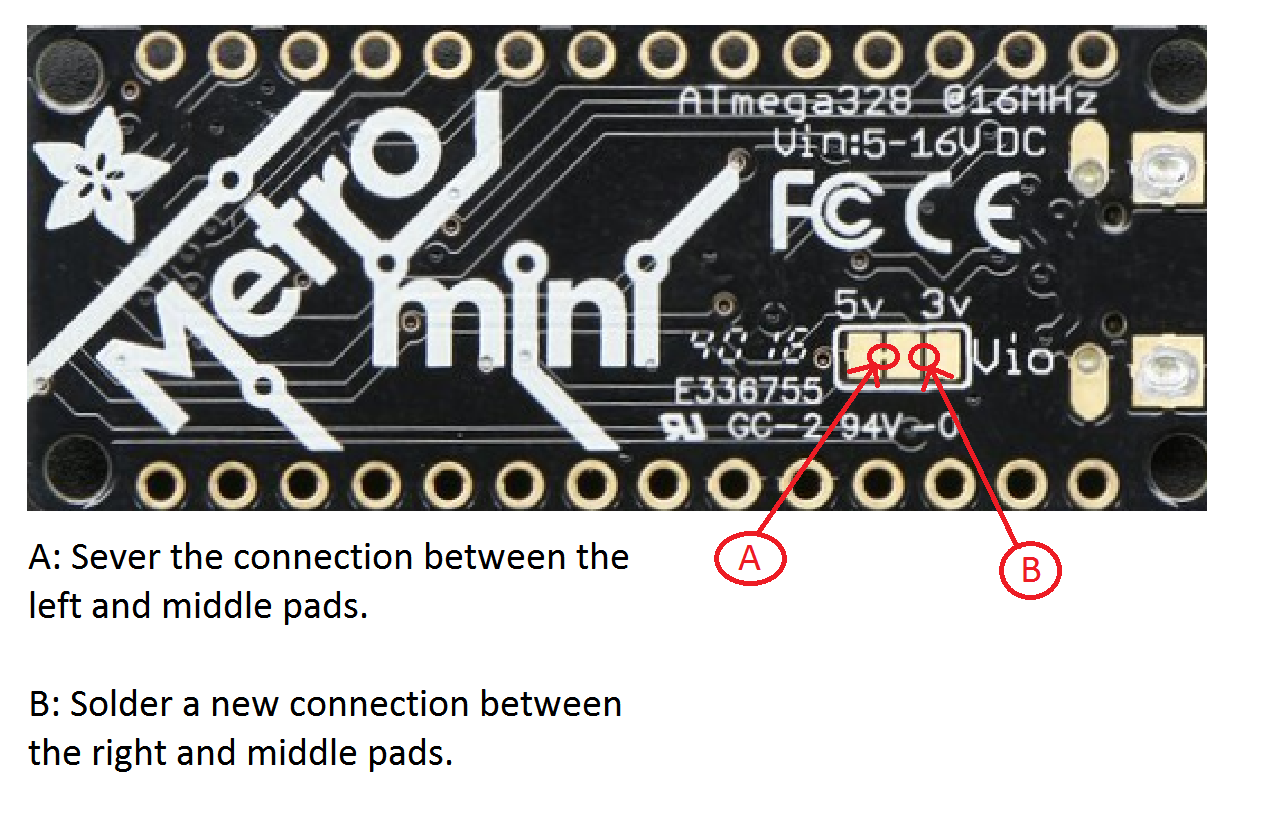
\includegraphics[scale=0.5]{mm_mod}}
\item{Modify IMUs to allow their AD0 pins to receive voltage which enables dynamic I2C addresses \\ 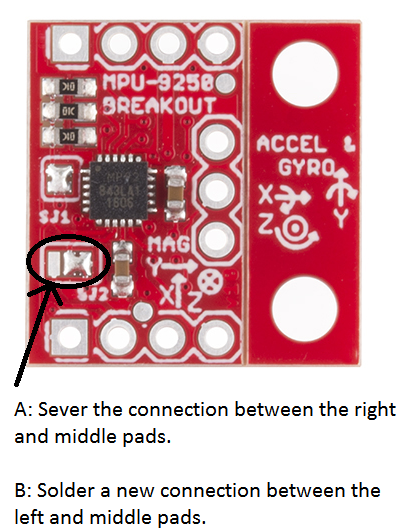
\includegraphics[scale=1.5]{mpu_mod}}
\item{Solder male headers to the bottom of the microcontroller}
\item{Solder male headers to the bottom of both IMUs}
\item{Attach the microcontroller and one IMU to the first breadboard}
\item{Attach the second IMU to the second breadboard}
\item{Connect devices and pc \\ 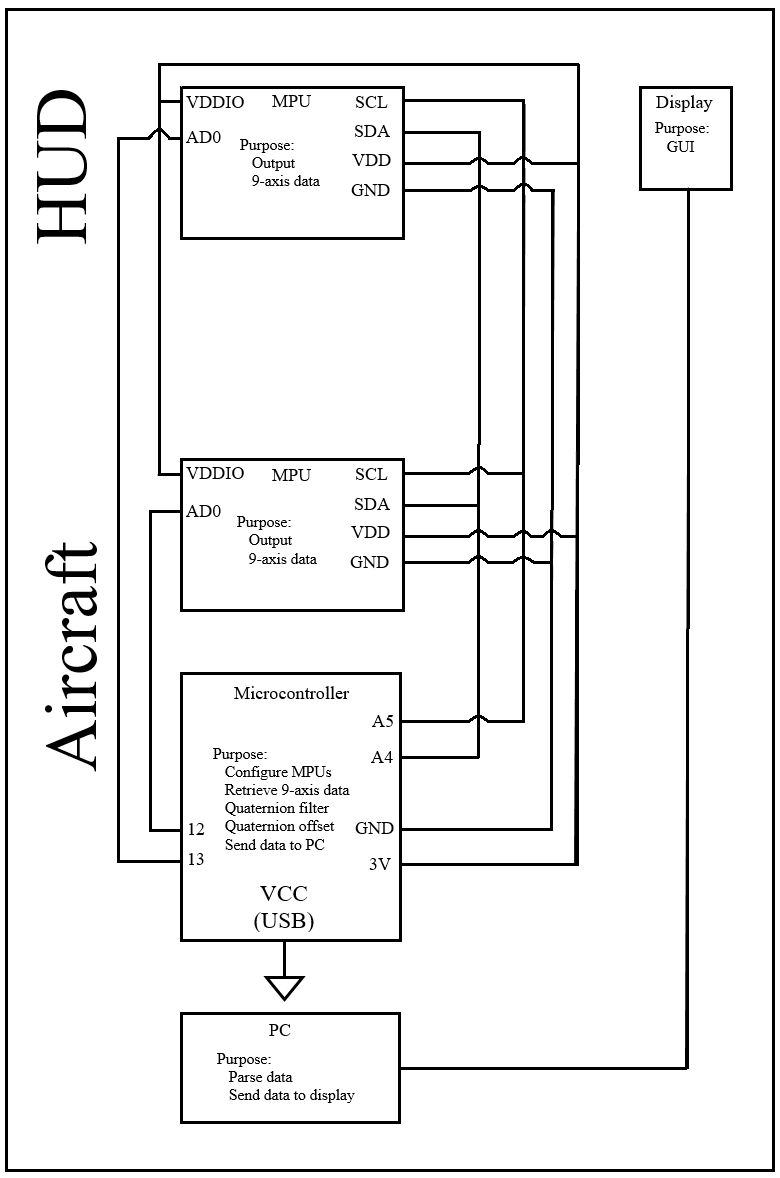
\includegraphics[scale=0.75]{Block_Diagram}}

\end{itemize}

\subsection*{Setup Dependencies}
\begin{itemize}
\item{Install the Arduino IDE}
\item{Install Python 2.7.9}
\item{Install VPython}
\item{Install pySerial}
\item{Download our arduino project}
\item{Download our python script}
\end{itemize}

\subsection*{Program Hardware}
\begin{itemize}
\item{Ensure that the microcontroller is connected to the PC}
\item{Load our arduino project on the Arduino IDE}
\item{Program the microcontroller with our project through the Arduino IDE}
\end{itemize}

\subsection*{Run application}
\begin{itemize}
\item{Load our python script}
\item{Run the script and follow instructions}
\item{Verify results by viewing the GUI}
\end{itemize}

\subsection*{PSEUDO CODE}
\begin{lstlisting}
// Place HUD in alignment with aircraft IRU
wait()
 
// Setup:
for each MPU-9250:
	update AD0 pin	// Do this in order to change I2C address
	initialize/configure registers
	for each sensor: // Accelerometer, Gyroscope, and magnetometer
		initialize/configure registers
calibrate device
 
// Install HUD
wait()
 
// Static Offset Mode
while statistical confidence insufficient:
	while sample size insufficient:
		for each MPU-9250:
			read data
			update stored quaternion value via quaternion filter
		record quaternion offset sample
	perform confidence interval
 
send static offset via serial port
 
// Dynamic offset mode
while system is active:
for each MPU-9250:
	read data
	update stored quaternion value via quaternion filter
record quaternion offset
 
send dynamic offset via serial port
\end{lstlisting}

\newpage
\section{How did we learn new Technology}


\newpage
\section{What did we learn from all this?}
	\subsection{Jiongcheng Luo}
		\begin{itemize}
			\item \textbf{What technical information did you learn?}
			\\ Throughout this course, a new technology I learned is Latex formatting. Throughout the project, I learned a lot about manufacturing an aircraft, especially its Head-up display system and Inertial Measurement Unit. I learned how an IMUs works and how we could apply it into a useful product. Specifically, from the perspective of software, I learned how to program Arduino and using VPython library.\\

			\item \textbf{What non-technical information did you learn?}
			\\I learned how to collaborate with a team from everyone did not know each other to everyone made a project together, specifically are the skills of communication, cooperation with co-workers. In addition, we had change to contact with a real company client, I learned a lot how a real industry deal with new technologies.  Throughout working on the project, I learned how to compare and choose the tools or technologies to be used for our project.\\

			\item \textbf{What have you learned about project work?}
			\\I learned that before doing a project, a team should have well discussion and make sure everyone understands what this project is doing. After that, a detailed, comprehensive plan needs to be made, during design procedures, all documents need to keep track of any changes and new ideas. During software development, using agile methodology is preferred, so that every part of the software can be modified easily.\\

			\item \textbf{What have you learned about project management?}
			\\A project first should be designed comprehensively including all details, graphs, diagrams, examples, documents etc. And during the implementation, it’s necessary to use version control for all software programs especially for a program that with complicated structure. Everyone can work on a different version for implementing different purpose or portion of the project, a completed version should a merge of all completed parts by different version and the merge needs to be agreed by all team members.\\

			\item \textbf{What have you learned about working in teams?}
			\\I learned that everyone in a team must has unique background knowledge, interests and everyone has different focus field, therefore, in order to get our project done successfully, we need to know each other well, including the lack and expertise of everyone, so that everyone can work on what they good at and everyone can complement for each other.\\

			\item \textbf{If you could do it all over, what would you do differently?}
			\\First, I would get started working on the project earlier, we had spent too much time on the design procedures and researching, then we found that we did not have enough time to accomplish the plans since more problems came up with we moving forward. Second, I would use version control system to keep track of our program, since we had met a problem that we did not save the previous version and we overwrote it, and as a result, we lose the version that was working before, so that we had to redo it all over again. Third, I would meet with our clients more often in regards to technical discussion, we had a lot of issues and problems that we did not know how to solve at all, and we had spent too much time in researching and attempting, that leads to that we could not complete some parts of the project at the end. Fourth, I would try using more IMUs for testing purpose, even though our result showed that working, it did not meet our initial expectation, more IMUs would more accurate.\\
		\end{itemize}

	\subsection{Drew Hamm}
		\begin{itemize}
			\item \textbf{What technical information did you learn?} \\
				This project ended up touching on quite a few topics that were previously unfamiliar to me.
				First, I had to learn about Tait-Bryan angles and how the different conventions worked such as for representing and aircrafts heading, elevation, and bank.
				Next, I had to learn about quaternions and several different filter algorithms, Madgwick and Mahony, for converting our 9-axis data into a usable form.
				Since our work focused primarily hardware, I had to learn how to configure and communicate with our devices; which required extensive reading into register mapping and other documentation.
				Additionally, I learned how to work with accelerometers, gyroscopes, and magnetometers.
				Lastly, I learned improved technical writing skills along with Latex formatting. \\

			\item \textbf{What non-technical information did you learn?} \\
				Primarily, throughout this project I had to learn how to work effectively with a new team.
				Communication amongst the team as well as with our client played heavily into our means to achieve a successful outcome.
				In order to complete tasks on time, especially after falling behind initially, improving my time management skills was crucial.
				Lastly, the skills required for expo such as communicating ideas from technical topics to diverse audiences. \\

			\item \textbf{What have you learned about project work?} \\
				Although I already knew of the importance that communication had in project work, I am now placing even greater emphasis on it for my later project work.
				I learned of the importance of creating tasks that can be developed independently.
				Creating tasks that can be effectively delegated amongst team members to play to everyone's strengths is something I would like to strive for in the future.
				Lastly, I learned how important a frequently updated timeline that includes milestones and well thought out tasks can be. \\

			\item \textbf{What have you learned about project management?} \\
				As for project management, I learned that it's important to keep a direct line of communication open between management and the team.
				Similarly to having a direct line of communication, it's important to maintain an updated timeline of the team's progression. \\

			\item \textbf{What have you learned about working in teams?} \\
				Since we made a poor first impression with our client, our team had to come together to overcome that initial problem.
				I learned how effective a united front could be to resolving issues. \\

			\item \textbf{If you could do it all over, what would you do differently?} \\
				First, I would like to setup version control early.
				Considering our project, there was some ambiguity as to whether we should develop in the open or not.
				Second, I would try to actively apply the skills I learned in my software development classes to promote collaboration and a sense of direction while building momentum as milestones were reached.
				Next, it would have been helpful to send more of my questions towards our client.
				By asking questions often, we could have improved our utilization of their technical experience to better guide my efforts.
				Unfortunately, we did not test our project soon enough and ended up going down a wrong path.
				If I had to do it all over, I would have tested early and often and considered following test driven development.
				Another change that would have greatly improved our results would have been to create an improved timeline that was updated frequently.
				An improved timeline would consist of tasks that could be developed independently.
				As with independent tasks, the timeline should consist of whom is responsible for which task; with proper thought put into each others strengths.
				Lastly, I would have tried to get access to not only the actual IRU that is used within an aircraft, but also the HUD that we were supposed to design our proof of concept solution for. \\
		\end{itemize}

	\subsection{Krisna Irawan}
	\begin{itemize}
			\item \textbf{What technical information did you learn?} \\
				I learned how MPU works. Before I took this course, I did not even know that this MPU is consist of gyroscope, accelerometer, and magnetometer. Taking this course was a huge learning curve for me. I also learned about quaternion, Proper Euler angles, and Tait–Bryan angles. I never learned about these concepts on any of my OSU classes and I learned it while working with this project. I also learn on how to use Vpython to create the graphical user interface. This language was straightforward and easier than OpenGL. I am glad that I learned it in this project. Lastly, I also learned to use LaTex. It was a steep learning curve, but it gets easier when you are used to it. \\

			\item \textbf{What non-technical information did you learn?} \\
				I learned to communicate effectively with my teammates. I learned to respect people time, especially our clients time. Communication is the most important thing during a huge group project like this. By working with a real industry client, Rockwell Collins, I also get a taste on how a real industry works. The documents that I wrote for this class taught me that project manager is not an easy job. Project manager has to deal with a lot of administration and documentation of the project, while at the same time, oversees the project. \\

			\item \textbf{What have you learned about project work?} \\
				I learned that planning is crucial for the success of the project. It was important for the team to be on the same page, and have the same goal. It was also important to consider that there is a risk in every step of the project. Thus, starting early and having an extra time on the schedule to work on the error was crucial. I also learned that documents that we wrote should reflect the changes on our project at all time, thus reducing any miscommunication between teammates.  \\

			\item \textbf{What have you learned about project management?} \\
				Documentations took a lot work and effort to do. However, documentations were also crucial for the success of the project. These documents were our main communication with the clients. Our clients gave valuable input and feedback based on these documents. Hence, it was important to keep it up to date. Version control was also important for the success of the team. A lot of time for debugging and merging can be reduced if we have a good version control. Also, by having a good version control, we can confidently work on a new concept without having a fear of losing or messing-up the previous work, and when we do messed-up, we can always go back to the old version. \\

			\item \textbf{What have you learned about working in teams?} \\
				Everybody in a team have their own weaknesses and strengths. To work well together as a team, it was important to know the strengths and weaknesses of each team member from early on. It was important for the team to have each other backs and complement each other. It was also important to communicate effectively and pro-actively. Effective communication was the key for a successful team project. \\

			\item \textbf{If you could do it all over, what would you do differently?} \\
				I would like to start early on the project. There were a lot of things that our team should learn for this project, which cuts down the implementation time of this project. I think by starting early, we can get some extra time to work on the implementation of this project. I also want to have a risk management plan while planning on the timeline for this project. It is important to consider that there is a risk in every step of the project. Thus, starting early and having an extra time on the schedule to work on the error was crucial. There were a lot of time where we created a tight schedule without even considering what would go wrong with that step of the project. When that step goes wrong, out team scramble all over the place and panic. This made us cut the next step implementation time to work on debugging the current step. This method was proven to be inefficient and stressful. Thus, if I could do it all over again, I would like to have a better risk management plan. \\
				
				Next, I also want to have a better version control. There was a time when we have a working version and start to work on the next implementation step. The next thing we know, the next implementation step did not work and we have no way to go back to the old version. It was frustrating for our team, trying to make the code work like it used to be. This experience makes me realize that version control is important. \\
				
				Finally, I want to have a better communication with the clients. During the last two terms, our meeting with the clients was minimal. I think this is caused by the lack of communication from our team to the clients. I think it is important to keep in touch with our clients on a weekly basis. A small email updates should be good to serve this purpose. In this email, our team can also ask the clients questions that we might have for the project. There was a lot of time where our team spend too much time on a problem without having any result. I think our clients’ technical expertise can guide us through this problem, and create more time for us to further refine the project. \\
		\end{itemize}





\newpage
\section{Appendix (Source Code)}

	\subsection{Note for source code}
	\begin{itemize}
		\item {There are totoally 12 .cpp code files for microntroller prgoram, 1 .ino code file as the main program for running arduino and 1 Python code file for graphical user interface. }
		
		\item {"MPU9250.cpp" and "MPU9250.h" are libraries for the MPU9250 IMU breakout.}

		\item {"quaternionFilters.cpp" and "quaternionFilters.h" are online credited libraries we found for quaternion convertion calculation.}

		\item {"quaternionFilters.cpp" and "quaternionFilters.h" are online credited libraries we found for quaternion convertion calculation.}
	\end{itemize}

	\begin{lstlisting}
# gui.py

	#!/usr/bin/python
	/*
	---	Oregon State University 2017 Capstone Project ---
	Author:		Jiongcheng Luo, Drew Hamm, Krisna Irawan
	Description:
		graphical display program using vpython (http://vpython.org/)
		and pyserial (https://pythonhosted.org/pyserial/) libraries
	*/

	import serial
	import visual as vp
	import math
	import sys
	import time 


	PORT = '/dev/tty.SLAB_USBtoUART'	# mac OS
	#PORT = 'COM4'						# windows


	BAUD_RATE = 38400
	DtoR = (math.pi/180)
	RtoD = (180/math.pi)

	SERIRAL_INPUT = serial.Serial(PORT, BAUD_RATE)


	def readData(string):
		newSerialInput = []
		for x in string.split(','):
			newSerialInput.append(x.strip())
		return newSerialInput

	#---------------------------------------------
	#				MAIN PROGRAM
	#---------------------------------------------
	class IMU():
		def __init__(self,name):
			self.name = name

			self.prev_pitch = 0
			self.prev_roll = 0
			self.prev_yaw = 0

			self.cur_pitch = 0		
			self.cur_roll = 0
			self.cur_yaw = 0

			self.pitch = 0		
			self.roll = 0
			self.yaw = 0

		def reset(self,b):
			if b == True:
				self.pitch = 0		
				self.roll = 0
				self.yaw = 0

	def reset(plane, yaw, pitch, roll, color):
		plane.visible = False
		del plane
		#time.sleep(0.05)
		plane = vp.frame()
		vp.ellipsoid(frame=plane, pos=(0,0,0), length=8, height=2.5, width=2.5, color=color, opacity=0.5)
		vp.pyramid(frame=plane, pos=(-1,0,0), size=(4,6,1), color=color, opacity=0.5)
		vp.pyramid(frame=plane, pos=(-3.5,0,1), size=(2,1,2), color=color, opacity=0.5)
		plane.rotate(angle=math.pi/2, axis=(-1,0,0), origin=(0,0,0))
		
		plane.rotate(angle=-math.pi/2, axis=(0,1,0))	
		plane.rotate(angle=roll, axis=(0,0,1))		
		plane.rotate(angle=pitch, axis=(1,0,0))	
		return plane;

	def text_reset(text, data, x, y, z):
		text.visible = False
		del text
		data = data*RtoD
		text = vp.label(pos=(x,y,z), text=str(data), height=10, border=0, font='sans', color=vp.color.green, box=0)
		return text; 		
		
	def display():
		# scene and object initilaizing
		scene2 = vp.display(title='Airplane Simulation',
	     x=0, y=0, width=800, height=600,
	     center=(0,0,8), autoscale = 1, background=vp.color.black)
		 
		#Text  
		text1 = vp.label(pos=(-4,-8,0), text='Yaw', height=18, border=0, font='sans', color=vp.color.green, box=0)
		text1 = vp.label(pos=(0,-8,0), text='Pitch', height=18, border=0, font='sans', color=vp.color.green, box=0)
		text1 = vp.label(pos=(4,-8,0), text='Roll', height=18, border=0, font='sans', color=vp.color.green, box=0)
		text1 = vp.label(pos=(-8,-9,0), text='HUD IMU Data:', height=10, border=0, font='sans', color=vp.color.green, box=0)
		text1 = vp.label(pos=(-8,-10,0), text='Airplane IMU Data:', height=10, border=0, font='sans', color=vp.color.green, box=0)
		
		#Plane 1
		plane = vp.frame()
		vp.ellipsoid(frame=plane, pos=(0,0,0), length=8, height=2.5, width=2.5, color=vp.color.red, opacity=0.5)
		vp.pyramid(frame=plane, pos=(-1,0,0), size=(4,6,1), color=vp.color.red, opacity=0.5)
		vp.pyramid(frame=plane, pos=(-3.5,0,1), size=(2,1,2), color=vp.color.red, opacity=0.5)
		plane.rotate(angle=math.pi/2, axis=(-1,0,0), origin=(0,0,0))
		#Axis Rotation for debugging purpose
		plane.rotate(angle=math.pi/2, axis=(0,-1,0), origin=(0,0,0))
		# plane.rotate(angle=math.pi/2, axis=(0,0,-1), origin=(0,0,0))
		
		#Plane 2
		plane2 = vp.frame()
		vp.ellipsoid(frame=plane2, pos=(0,0,0), length=8, height=2.5, width=2.5, color=vp.color.green, opacity=0.5)
		vp.pyramid(frame=plane2, pos=(-1,0,0), size=(4,6,1), color=vp.color.green, opacity=0.5)
		vp.pyramid(frame=plane2, pos=(-3.5,0,1), size=(2,1,2), color=vp.color.green, opacity=0.5)
		plane2.rotate(angle=math.pi/2, axis=(-1,0,0), origin=(0,0,0))
		#Axis Rotation for debugging purpose
		plane2.rotate(angle=math.pi/2, axis=(0,-1,0), origin=(0,0,0))
		# plane2.rotate(angle=math.pi/2, axis=(0,0,-1), origin=(0,0,0))
		
		#Axis and Horizon Line
		Axis = vp.label(pos=(0,0,7.5), text='Y', height=10, border=0, font='sans', color=vp.color.green, box=0)
		Axis = vp.arrow(pos=(0,0,0), axis=(7,0,0), shaftwidth=0.1, color=vp.color.green, opacity=0.5)
		Axis = vp.label(pos=(7.5,0,0), text='X', height=10, border=0, font='sans', color=vp.color.green, box=0)
		Axis = vp.arrow(pos=(0,0,0), axis=(0,7,0), shaftwidth=0.1, color=vp.color.green, opacity=0.5)
		Axis = vp.label(pos=(0,7.5,0), text='Z', height=10, border=0, font='sans', color=vp.color.green, box=0)
		Axis = vp.arrow(pos=(0,0,0), axis=(0,0,7), shaftwidth=0.1, color=vp.color.green, opacity=0.5)
		
		#Print Original Data	
		text2 = vp.label(pos=(-4,-9,0), text='Original Data', height=10, border=0, font='sans', color=vp.color.green, box=0)
		text3 = vp.label(pos=(0,-9,0), text='Original Data', height=10, border=0, font='sans', color=vp.color.green, box=0)
		text4 = vp.label(pos=(4,-9,0), text='Original Data', height=10, border=0, font='sans', color=vp.color.green, box=0)
				
		#Print Aligned Data	
		text5 = vp.label(pos=(-4,-10,0), text='Alignment Error', height=10, border=0, font='sans', color=vp.color.green, box=0)
		text6 = vp.label(pos=(0,-10,0), text='Alignment Error', height=10, border=0, font='sans', color=vp.color.green, box=0)
		text7 = vp.label(pos=(4,-10,0), text='Alignment Error', height=10, border=0, font='sans', color=vp.color.green, box=0)
		
	#---------------------------------------------
	#					GUI PART
	#---------------------------------------------
		def sense_filter(cur,prev):	# adjust animation sensitivity
			__SENSE = 0.005		# higher _SENSE = higher sensitivity
			delta = cur - prev
			if math.fabs(delta) > __SENSE:
				return delta
			return 0

		# enable which axis to run 
		yawAxis = True
		pitchAxis = True
		rollAxis = True

		imu1 = IMU('1')
		imu2 = IMU('2')

		# init = 0
		# loop over for animation
		while True:
			# performed rate for animation
			vp.rate(50)	
			while SERIRAL_INPUT.inWaiting() == 0:
				pass

			serial_line = SERIRAL_INPUT.readline()
			c = readData(serial_line)
			if len(c) == 6:	# filter out none numeric data input
				print c
				imu1.cur_yaw = float(c[3]) * DtoR
				imu1.cur_pitch = float(c[1]) * DtoR
				imu1.cur_roll = float(c[2]) * DtoR

				imu2.cur_yaw = float(c[3]) * DtoR
				imu2.cur_pitch = float(c[4]) * DtoR
				imu2.cur_roll = float(c[5]) * DtoR

			plane = reset(plane, imu1.cur_yaw, imu1.cur_pitch, imu1.cur_roll, vp.color.red)
			plane2 = reset(plane2, imu2.cur_yaw, imu2.cur_pitch, imu2.cur_roll, vp.color.green)
			text2 = text_reset(text2, imu1.cur_yaw, -4, -9, 0)
			text3 = text_reset(text3, imu1.cur_pitch, 0, -9, 0)
			text4 = text_reset(text4, imu1.cur_roll, 4, -9, 0 )
			text5 = text_reset(text5, imu2.cur_yaw, -4, -10, 0)
			text6 = text_reset(text6, imu2.cur_pitch, 0, -10, 0 )
			text7 = text_reset(text7, imu2.cur_roll, 4, -10, 0 )

		SERIRAL_INPUT.close() # Only executes once the loop exits


	if __name__ == "__main__":
		yawA = []
		# for loop allows serial reading for couple of seconds
		# to avoid error
		print "initializing..."
			

		serial_line = SERIRAL_INPUT.readline().rstrip()

		while (serial_line != 'DONE'):
			serial_line = SERIRAL_INPUT.readline().rstrip()
			print serial_line


		display()

	\end{lstlisting}

	\begin{lstlisting}
	/*
	Drew Hamm
	Jiongcheng Luo
	Krisna Irawan
	Project information:
	Auto_Alignment.ino
	CS462 CS Senior Capstone
	Fall 2017 - Spring 2017
	Group 65

	Program description:
	Initializes two SparkFun MPU-9250 Breakout boards to communicate with a Adafruit Metro Mini 328 - 5V 16MHz board.
	Communication via a single I2C channel.
	Initializes both MPU-9250s with onboard error correcting values.
	Both MPU-9250 accelerometer, gyroscope and magnetometer is requested by and sent to the Metro Mini 328.
	A sensor fusion algorithm is applied to data recieved from each MPU-2950.
	Data is converted into the quaternion form.
	The quaternion data from each sensor is used to find the realtime alignment offset between each MPU-9250.

	TODO:
	Output the error variance along with alignment offset data.
	Apply statistical analysis to alignment offset data until error variance is reduced to an acceptable range.
	Transition from finding and recording the initial alignment offset to finding the dynamic alignment offset.
	note: dynamic alignment offset is in regards to to airframe droop problem.

	Note:
	SDA and SCL should have external pull-up resistors (to 3.3V).
	10k resistors are on the EMSENSR-9250 breakout board.

	Hardware Devices:
	Adafruit Metro Mini 328 - 5V 16MHz  => MetroMini328
	SparkFun MPU-9250 Breakout          => MPU[0]
	SparkFun MPU-9250 Breakout          => MPU[1]

	Hardware Modifications:
	MetroMini328   -> Convert GPIO Logic level to 3.3V down from 5V
	            => Cut and solder closed a jumper on the bottom of the board
	MPU[0], MPU[1] -> Enable AD0 to control the I2C address
	            => Resolder the SJ2 jumper to connect the middle and left pads.

	Hardware Connections:
	MetroMini328(3.3v) -> (MPU[0], MPU[1])(VDD)
	MetroMini328(GND)  -> (MPU[0], MPU[1])(GND)
	MetroMini328(A4)   -> (MPU[0], MPU[1])(SDA)
	MetroMini328(A5)   -> (MPU[0], MPU[1])(SCL)
	MetroMini328(12)   -> MPU[0](AD0)
	MetroMini328(13)   -> MPU[1](AD0)
	*/
	#include "stdafx.h"

	#define YAW 0
	#define PITCH 1
	#define ROLL 2
	#define maxSample 60



	void output_mag();
	void output_gyro();
	void output_acc();
	void output_Yaw_Pitch_Roll();


	// The two digital login pins on the MetroMini328 that will be used
	// to set the AD0 pins of each MPU9250
	int AD0[2] = {12, 13};

	// The two mpus connected to the microcontroller
	// One should have their AD0 pin set HIGH wheras the other should
	// have their AD0 pin set LOW
	MPU9250 mpu[2];

	int numberOfMPUs = 2;
	float samples[maxSample];

	void setup()
	{ 
	// Begin Wire to enable I2C communication
	Wire.begin();
	delay(1000);

	// Begin Serial to enable recieve output from microcontroller to pc
	Serial.begin(38400);

	// Set AD0 pins for each MPU in order to change their address
	// Store the respective address within each individual IMU
	if(SERIAL_DEBUG){
	Serial.println("Set ADO pins");
	}

	for(int i = 0; i < numberOfMPUs; i++){
	// Set AD0 
	pinMode(AD0[i], OUTPUT);
	digitalWrite(AD0[i], i);
	delay(100);

	// Set address for each device per its ADO pin value
	if(i){
	  mpu[i].set_i2c_address(MPU9250_ADDRESS_ADO_1);
	}else{
	  mpu[i].set_i2c_address(MPU9250_ADDRESS_ADO_0);
	}
	}

	delay(100);

	// Setup both mpus
	if(SERIAL_DEBUG){
	Serial.println("Setup both MPUS");
	}
	for(int i = 0; i < numberOfMPUs; i++){
	mpu[i].initMPU9250();
	}

	if(1){
	Serial.println("DONE");
	}

	for(int i = 0; i < maxSample; i++){
	samples[i] = 0.0;
	}

	}
	int c_sample=0;

	unsigned long last = millis();
	unsigned long now = last;
	unsigned long change_in_time = 0;
	//unsigned long d_t = 100;
	unsigned long d_t = 20;

	bool gotDataFrom_A = 0;
	bool gotDataFrom_B = 0;
	bool q_diff_found = 0;
	bool static_offset_unknown = true;

	float yaw_confidence_level = 0.0;
	float pitch_confidence_level = 0.0;
	float roll_confidence_level = 0.0;
	float static_yaw_offset = 0.0;
	float static_pitch_offset = 0.0;
	float static_roll_offset = 0.0;
	float dynamic_yaw_offset = 0.0;
	float dynamic_pitch_offset = 0.0;
	float dynamic_roll_offset = 0.0;

	Quaternion *q_diff;
	float yaw_offset = 0.0;
	float pitch_offset = 0.0;
	float roll_offset = 0.0;
	float yaw = 0.0;
	float pitch = 0.0;
	float roll = 0.0;

	int axis = YAW;
	int j = 0;


	float g_x = 0.0;
	float g_y = 0.0;
	float g_z = 0.0;
	void loop()
	{
	for(int i = 0; i < numberOfMPUs; i++){

	// Check if new data as been accumulated
	if (mpu[i].hasData()){ 
	  //Serial.print(i);
	  //Serial.println(" has data");
	  mpu[i].retrieve_data();
	  if(i == 0){
	    gotDataFrom_A = 1;
	  }else{
	    gotDataFrom_B = 1;
	  }
	}

	//updates time and the quaternion
	mpu[i].updateQuaternion();

	if(gotDataFrom_A == 1 && gotDataFrom_B == 1){
	  q_diff_found = 1;
	  gotDataFrom_A = 0;
	  gotDataFrom_B = 0;
	  now = millis();
	  change_in_time = now - last;
	  if(change_in_time > d_t){
	    last = millis();
	    output_Yaw_Pitch_Roll();
	  }
	}

	/*
	if(static_offset_unknown){
	  // Take the difference from the latest samples
	  if(gotDataFrom_A == 1 && gotDataFrom_B == 1){
	    // Update flags
	    //q_diff_found = true;
	    gotDataFrom_A = 0;
	    gotDataFrom_B = 0;
	    //if(q_diff){
	    //  free(q_diff);
	    //  q_diff = NULL;
	    //}

	    //Get the next sample
	    switch(axis){
	      case YAW:
	        samples[c_sample] = (quaternionToYaw(mpu[0].q_m.q) - quaternionToYaw(mpu[1].q_m.q));
	        break;
	      case PITCH:
	        samples[c_sample] = (quaternionToPitch(mpu[0].q_m.q) - quaternionToYaw(mpu[1].q_m.q));
	        break;
	      case ROLL:
	        samples[c_sample] = (quaternionToRoll(mpu[0].q_m.q) - quaternionToRoll(mpu[1].q_m.q));
	        break;
	    }

	    //Update current sample count
	    c_sample = c_sample + 1;

	    //Check if last sample was received
	    if(c_sample == maxSample){

	      for(int k = 0; k < maxSample; k++){
	        Serial.println(samples[k]);
	      }
	      Serial.print("Max sample reached for ");
	      switch(axis){
	        case YAW:
	          Serial.println("yaw.");
	          break;

	        case PITCH:
	          Serial.println("pitch.");
	          break;

	        case ROLL:
	          Serial.println("roll.");
	          break;
	      }

	      //Get mean
	      float mean = getMean(samples, maxSample);
	      Serial.print("mean: ");
	      Serial.println(mean);

	      //Get standard deviation
	      float standard_deviation = getStandardDeviation(samples, mean, maxSample);
	      Serial.print("standard_deviation: ");
	      Serial.println(standard_deviation);
	      //Get confidence interval
	      float confidence_level = getConfidenceInterval(standard_deviation, maxSample, 1.96);

	      //Check confidence interval before continuing
	      //Output results when passing
	      if(confidence_level < 0.001){
	        switch(axis){
	          case YAW:
	            yaw_confidence_level = confidence_level;
	            static_yaw_offset = mean;
	            axis = PITCH;
	            c_sample = 0;

	            Serial.print("Yaw offset: ");
	            Serial.print(static_yaw_offset, 5);
	            Serial.print(" +- ");
	            Serial.println(yaw_confidence_level, 5);
	            break;
	          case PITCH:
	            pitch_confidence_level = confidence_level;
	            static_pitch_offset = mean;
	            axis = ROLL;
	            c_sample = 0;

	            Serial.print("Pitch offset: ");
	            Serial.print(static_pitch_offset, 5);
	            Serial.print(" +- ");
	            Serial.println(pitch_confidence_level, 5);
	            break;
	          case ROLL:
	            roll_confidence_level = confidence_level;
	            static_roll_offset = mean;
	            static_offset_unknown = false;

	            Serial.print("Roll offset: ");
	            Serial.print(static_roll_offset, 5);
	            Serial.print(" +- ");
	            Serial.println(roll_confidence_level, 5);
	            Serial.println("DONE");
	            numberOfMPUs = 1;
	            //free(samples);
	            break;
	        }
	      }else{
	        Serial.println("Confidence level insufficient");
	        c_sample = 0;
	      }//confidence interval
	    }//max sample reached
	  }//both have data
	}//static offset unknown
	else{
	  // Output data
	  now = millis();
	  change_in_time = now - last;
	  if(change_in_time > d_t){
	    last = millis();
	    yaw = quaternionToYaw(mpu[0].q_m.q);// * PI / 180.0f;
	    pitch = quaternionToPitch(mpu[0].q_m.q);// * PI / 180.0f;
	    roll = quaternionToRoll(mpu[0].q_m.q);//  * PI / 180.0f;

	    //Output 'Airplane data'
	    Serial.print(yaw, 5);
	    Serial.print(",");
	    Serial.print(pitch, 5);
	    Serial.print(",");
	    Serial.print(roll, 5);
	    Serial.print(",");
	    //Output 'Corrected data'
	    Serial.print(yaw + static_yaw_offset, 5);
	    Serial.print(",");
	    Serial.print(pitch + static_pitch_offset, 5);
	    Serial.print(",");
	    Serial.println(roll + static_roll_offset, 5);
	  }// d_t
	}
	*/
	}//for

	}//loop



	void output_mag(){
	Serial.print(mpu[0].mx);
	Serial.print(",");
	Serial.print(mpu[0].my);
	Serial.print(",");
	Serial.print(mpu[0].mz);
	Serial.print(",");
	Serial.print(mpu[1].mx);
	Serial.print(",");
	Serial.print(mpu[1].my);
	Serial.print(",");
	Serial.println(mpu[1].mz);
	}

	void output_gyro(){
	Serial.print(mpu[0].gy);
	Serial.print(",");
	Serial.println(mpu[1].gy);
	}

	void output_acc(){
	Serial.print(mpu[0].ax);
	Serial.print(",");
	Serial.print(mpu[0].ay);
	Serial.print(",");
	Serial.print(mpu[0].az);
	Serial.print(",");
	Serial.print(mpu[1].ax);
	Serial.print(",");
	Serial.print(mpu[1].ay);
	Serial.print(",");
	Serial.println(mpu[1].az);
	}

	void output_Yaw_Pitch_Roll(){
	float yaw_0 = quaternionToYaw(mpu[0].q_m.q) * RAD_TO_DEG;
	float pitch_0 = quaternionToPitch(mpu[0].q_m.q) * RAD_TO_DEG;
	float roll_0 = quaternionToRoll(mpu[0].q_m.q) * RAD_TO_DEG;
	float yaw_1 = quaternionToYaw(mpu[1].q_m.q) * RAD_TO_DEG;
	float pitch_1 = quaternionToPitch(mpu[1].q_m.q) * RAD_TO_DEG;
	float roll_1 = quaternionToRoll(mpu[1].q_m.q) * RAD_TO_DEG;
	Serial.print(yaw_0);
	Serial.print(",");
	Serial.print(pitch_0);
	Serial.print(",");
	Serial.print(roll_0);
	Serial.print(",");
	Serial.print(yaw_1);
	Serial.print(",");
	Serial.print(pitch_1);
	Serial.print(",");
	Serial.println(roll_1);
	}


	\end{lstlisting}

	\begin{lstlisting}
	/*

		data_utils.h

	*/
	#ifndef _DATAUTILS_H_
	#define _DATAUTILS_H_

	float getMean(float *samples, int sampleSize);
	float getStandardDeviation(float *samples, float mean, int sampleSize);
	float getConfidenceInterval(float standardDeviation, int sampleSize, float z_value);

	double quaternionToPhi(Quaternion *q);
	double quaternionToTheta(Quaternion *q);
	double quaternionToPsi(Quaternion *q);

	float quaternionToYaw(Quaternion *q);
	float quaternionToPitch(Quaternion *q);
	float quaternionToRoll(Quaternion *q);

	Quaternion* q_difference(Quaternion *q1, Quaternion *q2);

	Quaternion* q_inverse(Quaternion *q);
	Quaternion* q_conjugate(Quaternion *q);
	float q_dot(Quaternion *q1, Quaternion *q2);
	Quaternion* q_mult(Quaternion *q1, Quaternion *q2);
	Quaternion* q_div(Quaternion *q, float c);

	#endif

	\end{lstlisting}

	\begin{lstlisting}
	/*

		data_utils.cpp

	*/

	#include "stdafx.h"

	float getMean(float * samples, int sampleSize){
	  float mean = 0.0;
	  for(int i = 0; i < sampleSize; i++){
	    mean += samples[i];
	  }
	  mean = mean / sampleSize;
	  return mean;
	}

	float getStandardDeviation(float * samples, float mean, int sampleSize){
	  float standardDeviation = 0.0;
	  for(int i = 0; i < sampleSize; i++){
	    standardDeviation += (samples[i] - mean) * (samples[i] - mean);
	  }
	  standardDeviation = sqrt(standardDeviation / (float)sampleSize);
	  return standardDeviation;
	}

	float getConfidenceInterval(float standardDeviation, int sampleSize, float z_value){
	  float confidenceInterval = 0.0;
	  confidenceInterval = z_value * (standardDeviation / sqrt((float)sampleSize));
	  return confidenceInterval;
	}


	// Define output variables from updated quaternion---these are Tait-Bryan
	// angles, commonly used in aircraft orientation. In this coordinate system,
	// the positive z-axis is down toward Earth. Yaw is the angle between Sensor
	// x-axis and Earth magnetic North (or true North if corrected for local
	// declination, looking down on the sensor positive yaw is counterclockwise.
	// Pitch is angle between sensor x-axis and Earth ground plane, toward the
	// Earth is positive, up toward the sky is negative. Roll is angle between
	// sensor y-axis and Earth ground plane, y-axis up is positive roll. These
	// arise from the definition of the homogeneous rotation matrix constructed
	// from quaternions. Tait-Bryan angles as well as Euler angles are
	// non-commutative; that is, the get the correct orientation the rotations
	// must be applied in the correct order which for this configuration is yaw,
	// pitch, and then roll.
	// For more see
	// http://en.wikipedia.org/wiki/Conversion_between_quaternions_and_Euler_angles
	// which has additional links.

	//Returns yaw in radians
	float quaternionToYaw(Quaternion *q){
	  float q2q3 = q->q2 * q->q3;
	  float q1q4 = q->q1 * q->q4;
	  float q1q1 = q->q1 * q->q1;
	  float q2q2 = q->q2 * q->q2;
	  float q3q3 = q->q3 * q->q3;
	  float q4q4 = q->q4 * q->q4;
	  float yaw;
	  yaw = atan2f(2.0f * (q2q3 + q1q4), q1q1 + q2q2 - q3q3 - q4q4);

	  //Declination of corvallis
	  yaw += (15.14 * DEG_TO_RAD);

	  return yaw;
	}

	//Returns pitch in radians
	float quaternionToPitch(Quaternion *q){
	  float q2q4 = q->q2 * q->q4;
	  float q1q3 = q->q1 * q->q3;
	  float pitch;
	  pitch = -asinf(2.0f * (q2q4 - q1q3));

	  return pitch;
	}

	//Returns roll in radians
	float quaternionToRoll(Quaternion *q){
	  float q1q2 = q->q1 * q->q2;
	  float q3q4 = q->q3 * q->q4;
	  float q1q1 = q->q1 * q->q1;
	  float q2q2 = q->q2 * q->q2;
	  float q3q3 = q->q3 * q->q3;
	  float q4q4 = q->q4 * q->q4;

	  float roll;
	  roll = atan2f(2.0f * (q1q2 + q3q4), q1q1 - q2q2 - q3q3 + q4q4);

	  return roll;
	}


	double quaternionToPhi(Quaternion *q){
	  double q0 = q->q1;
	  double q1 = q->q2;
	  double q2 = q->q3;
	  double q3 = q->q4;

	  double R32 = 2.0 * (q2*q3 - q0*q1);
	  double R33 = 2.0 * q0*q0 - 1.0 + 2.0 * q3*q3;
	  double phi = atan2(R32, R33 );

	  return phi;
	}

	double quaternionToTheta(Quaternion *q){
	  double q0 = q->q1;
	  double q1 = q->q2;
	  double q2 = q->q3;
	  double q3 = q->q4;

	  double R31 = 2.0 * (q1*q3 + q0*q2);
	  double theta = -atan(R31 / sqrt(1.0 - R31*R31));

	  return theta;
	}

	double quaternionToPsi(Quaternion *q){
	  double q0 = q->q1;
	  double q1 = q->q2;
	  double q2 = q->q3;
	  double q3 = q->q4;

	  double R11 = 2.0 * q0*q0 - 1.0 + 2.0 * q1*q1;
	  double R21 = 2.0 * (q1*q2 - q0*q3);
	  double psi = atan2(R21, R11 );

	  return psi;

	}

	Quaternion* q_difference(Quaternion *q1, Quaternion *q2){
	  Quaternion *q_diff;
	  Quaternion *q_inv;
	  q_inv = q_inverse(q1);
	  q_diff = q_mult(q2, q_inv);

	  //Deconstruct
	  //q_inv
	  if(q_inv){
	    free(q_inv);
	    q_inv = NULL;
	  }

	  return q_diff;
	}

	Quaternion* q_inverse(Quaternion *q){
	  Quaternion *q_di;
	  Quaternion *q_co;
	  float dot = 1.0;
	  q_co = q_conjugate(q);
	  //dot = q_dot(q, q);
	  q_di = q_div(q_co, dot);

	  //Deconstruct
	  //q_co, q_do
	  if(q_co){
	    free(q_co);
	    q_co = NULL;
	  }
	  return q_di;
	}

	Quaternion* q_conjugate(Quaternion *q){
	  Quaternion *q_c = new Quaternion();
	  float q1 = q->q1;
	  float q2 = -(q->q2);
	  float q3 = -(q->q2);
	  float q4 = -(q->q2);

	  q_c->q1 = q1;
	  q_c->q2 = q2;
	  q_c->q3 = q3;
	  q_c->q4 = q4;

	  return q_c;
	}

	float q_dot(Quaternion *a, Quaternion *b){
	  float a1b1 = a->q1 * b->q1;
	  float a2b2 = a->q2 * b->q2;
	  float a3b3 = a->q3 * b->q3;
	  float a4b4 = a->q4 * b->q4;

	  float result = a1b1 + a2b2 + a3b3 + a4b4;
	  return result;
	}

	Quaternion* q_mult(Quaternion *a, Quaternion *b){
	  Quaternion *q_m = new Quaternion();
	  float a1b1 = a->q1 * b->q1;
	  float a2b2 = a->q2 * b->q2;
	  float a3b3 = a->q3 * b->q3;
	  float a4b4 = a->q4 * b->q4;

	  float a2b1 = a->q2 * b->q1;
	  float a1b2 = a->q1 * b->q2;
	  float a4b3 = a->q4 * b->q3;
	  float a3b4 = a->q3 * b->q4;

	  float a3b1 = a->q3 * b->q1;
	  float a4b2 = a->q4 * b->q2;
	  float a1b3 = a->q1 * b->q3;
	  float a2b4 = a->q2 * b->q4;

	  float a4b1 = a->q4 * b->q1;
	  float a3b2 = a->q3 * b->q2;
	  float a2b3 = a->q2 * b->q3;
	  float a1b4 = a->q1 * b->q4;

	  q_m->q1 = a1b1 - a2b2 - a3b3 - a4b4;
	  q_m->q2 = a2b1 + a1b2 - a4b3 + a3b4;
	  q_m->q3 = a3b1 + a4b2 + a1b3 - a2b4;
	  q_m->q4 = a4b1 - a3b2 + a2b3 + a1b4;
	  return q_m;
	}

	Quaternion* q_div(Quaternion *q, float c){
	  Quaternion *q_d = new Quaternion();
	  float q1_c = q->q1 / c;
	  float q2_c = q->q2 / c;
	  float q3_c = q->q3 / c;
	  float q4_c = q->q4 / c;

	  q_d->q1 = q1_c;
	  q_d->q2 = q2_c;
	  q_d->q3 = q3_c;
	  q_d->q4 = q4_c;

	  return q_d;
	}
	/*
	void q_print(Quaternion *q){
	  int precision = 5;
	  Serial.print("q1: ");
	  Serial.print(q -> q1, precision);
	  Serial.print(" q2: ");
	  Serial.print(q -> q2, precision);
	  Serial.print(" q3: ");
	  Serial.print(q -> q3, precision);
	  Serial.print(" q4: ");
	  Serial.println(q -> q4, precision);
	}
	*/

	\end{lstlisting}

	\begin{lstlisting}
	/*

		debug_config.h

	*/
	#ifndef _DEBUG_CONFIG_H_
	#define _DEBUG_CONFIG_H_

	#define SERIAL_DEBUG true
	#define EXTRA_GYRO_INFO false
	#endif

	\end{lstlisting}

	\begin{lstlisting}
	/*

		MPU9250.h

	*/


	/*
	 Note: The MPU9250 is an I2C sensor and uses the Arduino Wire library.
	 Because the sensor is not 5V tolerant, we are using a 3.3 V 8 MHz Pro Mini or
	 a 3.3 V Teensy 3.1. We have disabled the internal pull-ups used by the Wire
	 library in the Wire.h/twi.c utility file. We are also using the 400 kHz fast
	 I2C mode by setting the TWI_FREQ  to 400000L /twi.h utility file.
	 */
	#ifndef _MPU9250_H_
	#define _MPU9250_H_

	#define X_AXIS 0
	#define Y_AXIS 1
	#define Z_AXIS 2


	// See also MPU-9250 Register Map and Descriptions, Revision 4.0,
	// RM-MPU-9250A-00, Rev. 1.4, 9/9/2013 for registers not listed in above
	// document; the MPU9250 and MPU9150 are virtually identical but the latter has
	// a different register map

	//Magnetometer Registers
	#define AK8963_ADDRESS   0x0C
	#define WHO_AM_I_AK8963  0x00//0x49 // (AKA WIA) should return 0x48
	#define INFO             0x01
	#define AK8963_ST1       0x02  // data ready status bit 0
	#define AK8963_XOUT_L    0x03  // data
	#define AK8963_XOUT_H    0x04
	#define AK8963_YOUT_L    0x05
	#define AK8963_YOUT_H    0x06
	#define AK8963_ZOUT_L    0x07
	#define AK8963_ZOUT_H    0x08
	#define AK8963_ST2       0x09  // Data overflow bit 3 and data read error status bit 2
	#define AK8963_CNTL      0x0A  // Power down (0000), single-measurement (0001), self-test (1000) and Fuse ROM (1111) modes on bits 3:0
	#define AK8963_ASTC      0x0C  // Self test control
	#define AK8963_I2CDIS    0x0F  // I2C disable
	#define AK8963_ASAX      0x10  // Fuse ROM x-axis sensitivity adjustment value
	#define AK8963_ASAY      0x11  // Fuse ROM y-axis sensitivity adjustment value
	#define AK8963_ASAZ      0x12  // Fuse ROM z-axis sensitivity adjustment value

	#define AK8963_CNTL1      0x0A // Control 1 register
	#define AK8963_CNTL2      0x0B // Control 2 register

	// AK8963 Control Register Signals
	#define CNTL1_16BIT_OUTPUT 0x10
	#define CNTL1_CONTINUOUS_MEASUREMENT_MODE_1 0x02
	#define CNTL1_CONTINUOUS_MEASUREMENT_MODE_2 0x06 // 100Hz
	#define CNTL1_FUSE_ROM_MODE 0x0F
	#define CNTL2_SOFT_RESTART 0x01

	#define SELF_TEST_X_GYRO 0x00
	#define SELF_TEST_Y_GYRO 0x01
	#define SELF_TEST_Z_GYRO 0x02

	/*#define X_FINE_GAIN      0x03 // [7:0] fine gain
	#define Y_FINE_GAIN      0x04
	#define Z_FINE_GAIN      0x05
	#define XA_OFFSET_H      0x06 // User-defined trim values for accelerometer
	#define XA_OFFSET_L_TC   0x07
	#define YA_OFFSET_H      0x08
	#define YA_OFFSET_L_TC   0x09
	#define ZA_OFFSET_H      0x0A
	#define ZA_OFFSET_L_TC   0x0B */

	#define SELF_TEST_X_ACCEL 0x0D
	#define SELF_TEST_Y_ACCEL 0x0E
	#define SELF_TEST_Z_ACCEL 0x0F

	#define SELF_TEST_A       0x10

	#define XG_OFFSET_H       0x13  // User-defined trim values for gyroscope
	#define XG_OFFSET_L       0x14
	#define YG_OFFSET_H       0x15
	#define YG_OFFSET_L       0x16
	#define ZG_OFFSET_H       0x17
	#define ZG_OFFSET_L       0x18
	#define SMPLRT_DIV        0x19
	#define CONFIG            0x1A
	#define GYRO_CONFIG       0x1B
	#define ACCEL_CONFIG      0x1C
	#define ACCEL_CONFIG2     0x1D
	#define LP_ACCEL_ODR      0x1E
	#define WOM_THR           0x1F

	// Duration counter threshold for motion interrupt generation, 1 kHz rate,
	// LSB = 1 ms
	#define MOT_DUR           0x20
	// Zero-motion detection threshold bits [7:0]
	#define ZMOT_THR          0x21
	// Duration counter threshold for zero motion interrupt generation, 16 Hz rate,
	// LSB = 64 ms
	#define ZRMOT_DUR         0x22

	#define FIFO_EN            0x23
	#define I2C_MST_CTRL       0x24
	#define I2C_SLV0_ADDR      0x25
	#define I2C_SLV0_REG       0x26
	#define I2C_SLV0_CTRL      0x27
	#define I2C_SLV1_ADDR      0x28
	#define I2C_SLV1_REG       0x29
	#define I2C_SLV1_CTRL      0x2A
	#define I2C_SLV2_ADDR      0x2B
	#define I2C_SLV2_REG       0x2C
	#define I2C_SLV2_CTRL      0x2D
	#define I2C_SLV3_ADDR      0x2E
	#define I2C_SLV3_REG       0x2F
	#define I2C_SLV3_CTRL      0x30
	#define I2C_SLV4_ADDR      0x31
	#define I2C_SLV4_REG       0x32
	#define I2C_SLV4_DO        0x33
	#define I2C_SLV4_CTRL      0x34
	#define I2C_SLV4_DI        0x35
	#define I2C_MST_STATUS     0x36
	#define INT_PIN_CFG        0x37
	#define INT_ENABLE         0x38
	#define DMP_INT_STATUS     0x39  // Check DMP interrupt
	#define INT_STATUS         0x3A
	#define ACCEL_XOUT_H       0x3B
	#define ACCEL_XOUT_L       0x3C
	#define ACCEL_YOUT_H       0x3D
	#define ACCEL_YOUT_L       0x3E
	#define ACCEL_ZOUT_H       0x3F
	#define ACCEL_ZOUT_L       0x40
	#define TEMP_OUT_H         0x41
	#define TEMP_OUT_L         0x42
	#define GYRO_XOUT_H        0x43
	#define GYRO_XOUT_L        0x44
	#define GYRO_YOUT_H        0x45
	#define GYRO_YOUT_L        0x46
	#define GYRO_ZOUT_H        0x47
	#define GYRO_ZOUT_L        0x48
	#define EXT_SENS_DATA_00   0x49
	#define EXT_SENS_DATA_01   0x4A
	#define EXT_SENS_DATA_02   0x4B
	#define EXT_SENS_DATA_03   0x4C
	#define EXT_SENS_DATA_04   0x4D
	#define EXT_SENS_DATA_05   0x4E
	#define EXT_SENS_DATA_06   0x4F
	#define EXT_SENS_DATA_07   0x50
	#define EXT_SENS_DATA_08   0x51
	#define EXT_SENS_DATA_09   0x52
	#define EXT_SENS_DATA_10   0x53
	#define EXT_SENS_DATA_11   0x54
	#define EXT_SENS_DATA_12   0x55
	#define EXT_SENS_DATA_13   0x56
	#define EXT_SENS_DATA_14   0x57
	#define EXT_SENS_DATA_15   0x58
	#define EXT_SENS_DATA_16   0x59
	#define EXT_SENS_DATA_17   0x5A
	#define EXT_SENS_DATA_18   0x5B
	#define EXT_SENS_DATA_19   0x5C
	#define EXT_SENS_DATA_20   0x5D
	#define EXT_SENS_DATA_21   0x5E
	#define EXT_SENS_DATA_22   0x5F
	#define EXT_SENS_DATA_23   0x60
	#define MOT_DETECT_STATUS  0x61
	#define I2C_SLV0_DO        0x63
	#define I2C_SLV1_DO        0x64
	#define I2C_SLV2_DO        0x65
	#define I2C_SLV3_DO        0x66
	#define I2C_MST_DELAY_CTRL 0x67
	#define SIGNAL_PATH_RESET  0x68
	#define MOT_DETECT_CTRL    0x69
	#define USER_CTRL          0x6A  // Bit 7 enable DMP, bit 3 reset DMP
	#define PWR_MGMT_1         0x6B // Device defaults to the SLEEP mode
	#define PWR_MGMT_2         0x6C
	#define DMP_BANK           0x6D  // Activates a specific bank in the DMP
	#define DMP_RW_PNT         0x6E  // Set read/write pointer to a specific start address in specified DMP bank
	#define DMP_REG            0x6F  // Register in DMP from which to read or to which to write
	#define DMP_REG_1          0x70
	#define DMP_REG_2          0x71
	#define FIFO_COUNTH        0x72
	#define FIFO_COUNTL        0x73
	#define FIFO_R_W           0x74
	#define WHO_AM_I_MPU9250   0x75 // Should return 0x71
	#define XA_OFFSET_H        0x77
	#define XA_OFFSET_L        0x78
	#define YA_OFFSET_H        0x7A
	#define YA_OFFSET_L        0x7B
	#define ZA_OFFSET_H        0x7D
	#define ZA_OFFSET_L        0x7E

	//MPU9250 Slave Control Register Signals
	#define I2C_SLV0_EN        0x80

	// Using the MPU-9250 breakout board, ADO is set to 0
	// Seven-bit device address is 110100 for ADO = 0 and 110101 for ADO = 1
	#define MPU9250_ADDRESS_ADO_1 0x69  // Device address when ADO = 1
	#define MPU9250_ADDRESS_ADO_0 0x68  // Device address when ADO = 0
	#define AK8963_ADDRESS  0x0C   // Address of magnetometer

	#define READ_FLAG 0x80

	class MPU9250
	{
	  private:
	    uint8_t delay_s = 10;
	    uint8_t delay_m = 35;
	    uint8_t delay_l = 100;

	    bool read_Magnetometer();
	    bool read_Accelerometer();
	    bool read_Gyroscope();
	    bool initMPU9250_Magnetometer();
	    bool initMPU9250_Accelerometer();
	    bool initMPU9250_Gyroscope();
	    bool calibrateMPU9250_Magnetometer();
	    bool calibrateMPU9250_Accelerometer();
	    bool calibrateMPU9250_Gyroscope();

	  protected:
	    uint8_t i2c_address = MPU9250_ADDRESS_ADO_0;

	    // Set initial input parameters
	    enum Ascale
	    {
	      AFS_2G = 0,
	      AFS_4G,
	      AFS_8G,
	      AFS_16G
	    };

	    enum Gscale {
	      GFS_250DPS = 0,
	      GFS_500DPS,
	      GFS_1000DPS,
	      GFS_2000DPS
	    };

	    enum Mscale {
	      MFS_14BITS = 0, // 0.6 mG per LSB
	      MFS_16BITS      // 0.15 mG per LSB
	    };

	    enum M_MODE {
	      M_8HZ = 0x02,  // 8 Hz update
	      M_100HZ = 0x06 // 100 Hz continuous magnetometer
	    };

	    // TODO: Add setter methods for this hard coded stuff
	    // Specify sensor full scale
	    uint8_t Gscale = GFS_250DPS;
	    uint8_t Ascale = AFS_2G;
	    // Choose either 14-bit or 16-bit magnetometer resolution
	    uint8_t Mscale = MFS_16BITS;

	    // 2 for 8 Hz, 6 for 100 Hz continuous magnetometer data read
	    uint8_t Mmode = M_100HZ;

	  public:
	    Quaternion_Module q_m;

	    float temperature;   // Stores the real internal chip temperature in Celsius
	    int16_t tempCount;   // Temperature raw count output

	    // Stores the 16-bit signed sensor outputs
	    int16_t accelCount[3], gyroCount[3], magCount[3];

	    // Scale resolutions per LSB for the sensors
	    float aRes, gRes, mRes;

	    // Variables to hold latest sensor data values
	    float ax, ay, az, gx, gy, gz, mx, my, mz;

	    // Factory mag calibration and mag bias
	    float factoryMagCalibration[3] = {0, 0, 0}, factoryMagBias[3] = {0, 0, 0};

	    // Bias corrections for gyro, accelerometer, and magnetometer
	    float gyroBias[3]  = {0, 0, 0},
	          accelBias[3] = {0, 0, 0},
	          magBias[3]   = {0, 0, 0},
	          magScale[3]  = {0, 0, 0};
	    float selfTest[6];

	    // Public method declarations
	    void getMres();
	    void getAres();
	    void getGres();
	    uint16_t getSampleCount();
	    uint16_t getSampleDelay();
	    uint8_t writeByte(uint8_t, uint8_t, uint8_t);
	    uint8_t readByte(uint8_t, uint8_t);
	    uint8_t readBytes(uint8_t, uint8_t, uint8_t, uint8_t *);
	    uint8_t getAscale();
	    uint8_t getGscale();
	    uint8_t getMscale();
	    uint8_t getM_Mode();

	    bool set_i2c_address(uint8_t address);
	    void initMPU9250();
	    bool hasData();
	    void retrieve_data();
	    
	    void updateQuaternion();
	};

	#endif // _MPU9250_H_
	\end{lstlisting}

	\begin{lstlisting}
	/*

		MPU9250.cpp

	*/
	#include "stdafx.h"

	//==============================================================================
	//====== Set of useful function to access acceleration. gyroscope, magnetometer,
	//====== and temperature data
	//==============================================================================

	// If intPin goes high, all data registers have new data
	// On interrupt, check if data ready interrupt
	bool MPU9250::hasData(){
	  return (readByte(i2c_address, INT_STATUS) & 0x01);
	}

	void MPU9250::getMres()
	{
	  switch (Mscale)
	  {
	    // Possible magnetometer scales (and their register bit settings) are:
	    // 14 bit resolution (0) and 16 bit resolution (1)
	    case MFS_14BITS:
	      mRes = 10.0f * 4912.0f / 8190.0f; // Proper scale to return milliGauss
	      break;
	    case MFS_16BITS:
	      mRes = 10.0f * 4912.0f / 32760.0f; // Proper scale to return milliGauss
	      break;
	  }
	}

	void MPU9250::getGres()
	{
	  switch (Gscale)
	  {
	    // Possible gyro scales (and their register bit settings) are:
	    // 250 DPS (00), 500 DPS (01), 1000 DPS (10), and 2000 DPS (11).
	    // Here's a bit of an algorith to calculate DPS/(ADC tick) based on that
	    // 2-bit value:
	    case GFS_250DPS:
	      gRes = 250.0f / 32768.0f;
	      break;
	    case GFS_500DPS:
	      gRes = 500.0f / 32768.0f;
	      break;
	    case GFS_1000DPS:
	      gRes = 1000.0f / 32768.0f;
	      break;
	    case GFS_2000DPS:
	      gRes = 2000.0f / 32768.0f;
	      break;
	  }
	}

	void MPU9250::getAres()
	{
	  switch (Ascale)
	  {
	    // Possible accelerometer scales (and their register bit settings) are:
	    // 2 Gs (00), 4 Gs (01), 8 Gs (10), and 16 Gs  (11).
	    // Here's a bit of an algorith to calculate DPS/(ADC tick) based on that
	    // 2-bit value:
	    case AFS_2G:
	      aRes = 2.0f / 32768.0f;
	      break;
	    case AFS_4G:
	      aRes = 4.0f / 32768.0f;
	      break;
	    case AFS_8G:
	      aRes = 8.0f / 32768.0f;
	      break;
	    case AFS_16G:
	      aRes = 16.0f / 32768.0f;
	      break;
	  }
	}

	uint8_t MPU9250::getAscale(){
	  return Ascale;
	}

	uint8_t MPU9250::getGscale(){
	  return Gscale;
	}

	uint8_t MPU9250::getMscale(){
	  return Mscale;
	}

	uint8_t MPU9250::getM_Mode(){
	  return Mmode;
	}

	uint16_t MPU9250::getSampleCount(){
	  uint16_t sample_count = 0;
	  // shoot for ~fifteen seconds of mag data
	  // at 8 Hz ODR, new mag data is available every 125 ms
	  if (Mmode == M_8HZ)
	  {
	    sample_count = 128;
	  }
	  // at 100 Hz ODR, new mag data is available every 10 ms
	  if (Mmode == M_100HZ)
	  {
	    sample_count = 1500;
	  }

	  return sample_count;
	}

	uint16_t MPU9250::getSampleDelay(){
	  uint16_t sample_delay = 0;

	  if (Mmode == M_8HZ)
	  {
	    sample_delay = 135; // At 8 Hz ODR, new mag data is available every 125 ms
	  }
	  if (Mmode == M_100HZ)
	  {
	    sample_delay = 12;  // At 100 Hz ODR, new mag data is available every 10 ms
	  }

	  return sample_delay;
	}


	bool MPU9250::set_i2c_address(uint8_t address){
	  i2c_address = address;
	}

	bool MPU9250::initMPU9250_Magnetometer(){
	  // First extract the factory calibration for each magnetometer axis
	  uint8_t rawData[3];  // x/y/z gyro calibration data stored here

	  // Point to magnetometer before writing data
	  // Set to write to slave address AK8963_ADDRESS
	  writeByte(i2c_address, I2C_SLV0_ADDR, AK8963_ADDRESS);
	  delay(delay_s);
	  
	  // Now point to a megnetometer register that data will be written to
	  // Point slave 0 register at AK8963's control 2 (soft reset) register
	  writeByte(i2c_address, I2C_SLV0_REG, AK8963_CNTL2);
	  delay(delay_s);

	  // Send data
	  // Soft restart via AK8963's control 2
	  writeByte(i2c_address, I2C_SLV0_DO, CNTL2_SOFT_RESTART);
	  delay(delay_s);

	  // Point to a different magnetometer register for a seperate write
	  // Point slave 0 register at AK8963's control 1 (mode) register
	  writeByte(i2c_address, I2C_SLV0_REG, AK8963_CNTL1);
	  delay(delay_s);
	  
	  // Send data
	  // Enter Fuse ROM access mode
	  writeByte(i2c_address, I2C_SLV0_DO, CNTL1_FUSE_ROM_MODE);
	  delay(delay_s);

	  // Enable read from magnometer
	  // Set to read from slave address AK8963_ADDRESS
	  writeByte(i2c_address, I2C_SLV0_ADDR, AK8963_ADDRESS | READ_FLAG);
	  delay(delay_s);

	  // Now point to a megnetometer register that data will be read from
	  // Point slave 0 register at AK8963's fuse rom x-axis
	  writeByte(i2c_address, I2C_SLV0_REG, AK8963_ASAX);
	  delay(delay_s);

	  // Enable simple 3-byte I2C read from slave 0
	  writeByte(i2c_address, I2C_SLV0_CTRL, READ_FLAG | 0x03);
	  delay(delay_l);

	  // Read the x-, y-, and z-axis calibration values
	  readBytes(i2c_address, EXT_SENS_DATA_00, 3, &rawData[0]);
	  delay(delay_l);

	  if(SERIAL_DEBUG){
	    Serial.print("rawData[0]: "); Serial.print(rawData[0]);
	    Serial.print(" ");
	    Serial.print("rawData[1]: "); Serial.print(rawData[1]);
	    Serial.print(" ");
	    Serial.print("rawData[2]: "); Serial.print(rawData[2]);
	    Serial.println("");
	  }

	  //Return x-axis sensitivity adjustment values, etc.
	  factoryMagCalibration[0] =  (float)(rawData[0] - 128)/256. + 1.;
	  factoryMagCalibration[1] =  (float)(rawData[1] - 128)/256. + 1.;
	  factoryMagCalibration[2] =  (float)(rawData[2] - 128)/256. + 1.;

	  if(SERIAL_DEBUG){
	    for(int i = 0; i < 3; i++){
	    Serial.print("factoryMagCalibration[");
	    Serial.print(i);
	    Serial.print("]: ");
	    Serial.print(factoryMagCalibration[i]);
	    Serial.println();
	    }
	  }

	  // Set to write to slave address AK8963_ADDRESS
	  writeByte(i2c_address, I2C_SLV0_ADDR, AK8963_ADDRESS);
	  delay(delay_s);
	  
	  // Point slave 0 register at AK8963's control 1 (mode) register
	  writeByte(i2c_address, I2C_SLV0_REG, AK8963_CNTL1);
	  delay(delay_s);

	  // 16-bit continuous measurement mode via AK8963's control 1
	  writeByte(i2c_address, I2C_SLV0_DO, Mscale << 4 | Mmode);
	  //writeByte(i2c_address, I2C_SLV0_DO, (CNTL1_16BIT_OUTPUT | CNTL1_CONTINUOUS_MEASUREMENT_MODE_2));
	  delay(delay_l);

	  // Setup for read
	  writeByte(i2c_address, I2C_SLV0_ADDR, AK8963_ADDRESS | READ_FLAG);

	  // Setup to read actual mag data
	  // Point slave to the data regs
	  writeByte(i2c_address, I2C_SLV0_REG, AK8963_XOUT_L);
	  delay(delay_s);

	  // Enable simple 7-byte I2C reads from slave 0
	  writeByte(i2c_address, I2C_SLV0_CTRL, READ_FLAG | 0x07);
	  delay(delay_s);

	}

	bool MPU9250::initMPU9250_Accelerometer(){
	  // Set accelerometer full-scale range configuration
	  // Get current ACCEL_CONFIG register value
	  uint8_t c = readByte(i2c_address, ACCEL_CONFIG);
	  // c = c & ~0xE0; // Clear self-test bits [7:5]
	  c = c & ~0x18;  // Clear AFS bits [4:3]
	  c = c | getAscale() << 3; // Set full scale range for the accelerometer
	  // Write new ACCEL_CONFIG register value
	  writeByte(i2c_address, ACCEL_CONFIG, c);

	  // Set accelerometer sample rate configuration
	  // It is possible to get a 4 kHz sample rate from the accelerometer by
	  // choosing 1 for accel_fchoice_b bit [3]; in this case the bandwidth is
	  // 1.13 kHz
	  // Get current ACCEL_CONFIG2 register value
	  c = readByte(i2c_address, ACCEL_CONFIG2);
	  c = c & ~0x0F; // Clear accel_fchoice_b (bit 3) and A_DLPFG (bits [2:0])
	  c = c | 0x03;  // Set accelerometer rate to 1 kHz and bandwidth to 41 Hz
	  // Write new ACCEL_CONFIG2 register value
	  writeByte(i2c_address, ACCEL_CONFIG2, c);
	}

	bool MPU9250::initMPU9250_Gyroscope(){
	  // Configure Gyro and Thermometer
	  // Disable FSYNC and set thermometer and gyro bandwidth to 41 and 42 Hz,
	  // respectively;
	  // minimum delay time for this setting is 5.9 ms, which means sensor fusion
	  // update rates cannot be higher than 1 / 0.0059 = 170 Hz
	  // DLPF_CFG = bits 2:0 = 011; this limits the sample rate to 1000 Hz for both
	  // With the MPU9250, it is possible to get gyro sample rates of 32 kHz (!),
	  // 8 kHz, or 1 kHz
	  writeByte(i2c_address, CONFIG, 0x03);

	  // Set sample rate = gyroscope output rate/(1 + SMPLRT_DIV)
	  // Use a 200 Hz rate; a rate consistent with the filter update rate
	  // determined inset in CONFIG above.
	  writeByte(i2c_address, SMPLRT_DIV, 0x04);

	  // Set gyroscope full scale range
	  // Range selects FS_SEL and AFS_SEL are 0 - 3, so 2-bit values are
	  // left-shifted into positions 4:3

	  // get current GYRO_CONFIG register value
	  uint8_t c = readByte(i2c_address, GYRO_CONFIG);
	  // c = c & ~0xE0; // Clear self-test bits [7:5]
	  c = c & ~0x03; // Clear Fchoice bits [1:0]
	  c = c & ~0x18; // Clear AFS bits [4:3]
	  c = c | getGscale() << 3; // Set full scale range for the gyro
	  // Set Fchoice for the gyro to 11 by writing its inverse to bits 1:0 of
	  // GYRO_CONFIG
	  // c =| 0x00;
	  // Write new GYRO_CONFIG value to register
	  writeByte(i2c_address, GYRO_CONFIG, c );

	}

	//Copied from xxx
	bool MPU9250::calibrateMPU9250_Magnetometer(){
	  uint16_t ii = 0, sample_count = 0, sample_delay = 0;
	  int32_t mag_bias[3]  = {0, 0, 0},
	          mag_scale[3] = {0, 0, 0};
	  int16_t mag_max[3]  = {0x8000, 0x8000, 0x8000},
	          mag_min[3]  = {0x7FFF, 0x7FFF, 0x7FFF};

	  // Make sure resolution has been calculated
	  getMres();

	  // if(SERIAL_DEBUG){
	  //   Serial.println(F("Mag Calibration: Wave device in a figure 8 until done!"));
	  //   Serial.println(F("  4 seconds to get ready followed by 15 seconds of sampling)"));
	  // }
	  delay(4000);

	  // Determine the number of samples to take
	  sample_count = 128;//getSampleCount();

	  // Determine the delay between each sample
	  sample_delay = getSampleDelay();

	  for (ii = 0; ii < sample_count; ii++)
	  {
	    read_Magnetometer();

	    for (int jj = 0; jj < 3; jj++)
	    {
	      if (magCount[jj] > mag_max[jj])
	      {
	        mag_max[jj] = magCount[jj];
	      }
	      if (magCount[jj] < mag_min[jj])
	      {
	        mag_min[jj] = magCount[jj];
	      }
	    }

	    delay(13);
	  }

	  if(SERIAL_DEBUG){
	    Serial.println("mag x min/max:"); Serial.println(mag_max[0]); Serial.println(mag_min[0]);
	    Serial.println("mag y min/max:"); Serial.println(mag_max[1]); Serial.println(mag_min[1]);
	    Serial.println("mag z min/max:"); Serial.println(mag_max[2]); Serial.println(mag_min[2]);
	  }

	  // Get hard iron correction
	  // Get 'average' x mag bias in counts
	  mag_bias[0]  = (mag_max[0] + mag_min[0]) / 2;
	  // Get 'average' y mag bias in counts
	  mag_bias[1]  = (mag_max[1] + mag_min[1]) / 2;
	  // Get 'average' z mag bias in counts
	  mag_bias[2]  = (mag_max[2] + mag_min[2]) / 2;

	  // Save mag biases in G for main program
	  magBias[0] = (float)mag_bias[0] * mRes * factoryMagCalibration[0];
	  magBias[1] = (float)mag_bias[1] * mRes * factoryMagCalibration[1];
	  magBias[2] = (float)mag_bias[2] * mRes * factoryMagCalibration[2];

	  // Get soft iron correction estimate
	  // Get average x axis max chord length in counts
	  mag_scale[0]  = (mag_max[0] - mag_min[0]) / 2;
	  // Get average y axis max chord length in counts
	  mag_scale[1]  = (mag_max[1] - mag_min[1]) / 2;
	  // Get average z axis max chord length in counts
	  mag_scale[2]  = (mag_max[2] - mag_min[2]) / 2;

	  float avg_rad = mag_scale[0] + mag_scale[1] + mag_scale[2];
	  avg_rad /= 3.0;

	  magScale[0] = avg_rad / ((float)mag_scale[0]);
	  magScale[1] = avg_rad / ((float)mag_scale[1]);
	  magScale[2] = avg_rad / ((float)mag_scale[2]);

	  if(SERIAL_DEBUG){
	    Serial.println(F("Mag Calibration done!"));
	  }
	}

	bool MPU9250::calibrateMPU9250_Accelerometer(){
	  uint8_t data[6]; // data array to hold accelerometer data
	  uint16_t ii, packet_count, fifo_count;
	  int32_t accel_bias[3] = {0, 0, 0};
	  int16_t acc_max[3]  = {0x8000, 0x8000, 0x8000},
	          acc_min[3]  = {0x7FFF, 0x7FFF, 0x7FFF};

	  if(SERIAL_DEBUG){
	    Serial.println("calibrateMPU9250_Accelerometer");
	  }

	  // Make sure resolution has been calculated
	  getAres();

	  // reset device
	  // Write a one to bit 7 reset bit; toggle reset device
	  writeByte(i2c_address, PWR_MGMT_1, READ_FLAG);
	  delay(100);

	  // get stable time source; Auto select clock source to be PLL gyroscope
	  // reference if ready else use the internal oscillator, bits 2:0 = 001
	  writeByte(i2c_address, PWR_MGMT_1, 0x01);
	  writeByte(i2c_address, PWR_MGMT_2, 0x00);
	  delay(200);

	  // Configure device for bias calculation
	  // Disable all interrupts
	  writeByte(i2c_address, INT_ENABLE, 0x00);
	  // Disable FIFO
	  writeByte(i2c_address, FIFO_EN, 0x00);
	  // Turn on internal clock source
	  writeByte(i2c_address, PWR_MGMT_1, 0x00);
	  // Disable I2C master
	  writeByte(i2c_address, I2C_MST_CTRL, 0x00);
	  // Disable FIFO and I2C master modes
	  writeByte(i2c_address, USER_CTRL, 0x00);
	  // Reset FIFO and DMP
	  writeByte(i2c_address, USER_CTRL, 0x0C);
	  delay(15);

	  // Configure MPU6050 gyro and accelerometer for bias calculation
	  // Set low-pass filter to 188 Hz
	  writeByte(i2c_address, CONFIG, 0x01);
	  // Set sample rate to 1 kHz
	  writeByte(i2c_address, SMPLRT_DIV, 0x00);
	  // Set accelerometer full-scale to 2 g, maximum sensitivity
	  writeByte(i2c_address, ACCEL_CONFIG, 0x00);

	  uint16_t  accelsensitivity = 16384; // = 16384 LSB/g

	  // Configure FIFO to capture accelerometer data for bias calculation
	  writeByte(i2c_address, USER_CTRL, 0x40);  // Enable FIFO
	  // Enable accelerometer sensors for FIFO  (max size 512 bytes in
	  // MPU-9150)
	  writeByte(i2c_address, FIFO_EN, 0x08);
	  delay(80);  // accumulate 80 samples in 80 milliseconds = 480 bytes

	  // At end of sample accumulation, turn off FIFO sensor read
	  // Disable accelerometer sensors for FIFO
	  writeByte(i2c_address, FIFO_EN, 0x00);
	  // Read FIFO sample count
	  readBytes(i2c_address, FIFO_COUNTH, 2, &data[0]);
	  fifo_count = ((uint16_t)data[0] << 8) | data[1];
	  // How many sets of full accelerometer data for averaging

	  packet_count = fifo_count/6;
	  if(SERIAL_DEBUG){
	    Serial.print("fifo_count: ");
	    Serial.println(fifo_count);
	    Serial.print("packet_count: ");
	    Serial.println(packet_count);
	  }

	  for (ii = 0; ii < packet_count; ii++)
	  {
	    int16_t accel_temp[3] = {0, 0, 0};
	    // Read data for averaging
	    readBytes(i2c_address, FIFO_R_W, 6, &data[0]);
	    // Form signed 16-bit integer for each sample in FIFO
	    accel_temp[0] = (int16_t) (((int16_t)data[0] << 8) | data[1]  );
	    accel_temp[1] = (int16_t) (((int16_t)data[2] << 8) | data[3]  );
	    accel_temp[2] = (int16_t) (((int16_t)data[4] << 8) | data[5]  );

	    // Sum individual signed 16-bit biases to get accumulated signed 32-bit
	    // biases.
	    accel_bias[0] += (int32_t) accel_temp[0];
	    accel_bias[1] += (int32_t) accel_temp[1];
	    accel_bias[2] += (int32_t) accel_temp[2];

	    for (int jj = 0; jj < 3; jj++)
	    {
	      if (accel_temp[jj] > acc_max[jj])
	      {
	        acc_max[jj] = accel_temp[jj];
	      }
	      if (accel_temp[jj] < acc_min[jj])
	      {
	        acc_min[jj] = accel_temp[jj];
	      }
	    }
	  }

	  if(SERIAL_DEBUG){
	    Serial.println("acc x min/max:"); Serial.println(acc_max[0]); Serial.println(acc_min[0]);
	    Serial.println("acc y min/max:"); Serial.println(acc_max[1]); Serial.println(acc_min[1]);
	    Serial.println("acc z min/max:"); Serial.println(acc_max[2]); Serial.println(acc_min[2]);
	  }

	  // Sum individual signed 16-bit biases to get accumulated signed 32-bit biases
	  accel_bias[0] /= (int32_t) packet_count;
	  accel_bias[1] /= (int32_t) packet_count;
	  accel_bias[2] /= (int32_t) packet_count;

	  // Sum individual signed 16-bit biases to get accumulated signed 32-bit biases
	  if (accel_bias[2] > 0L)
	  {
	    accel_bias[2] -= (int32_t) accelsensitivity;
	  }
	  else
	  {
	    accel_bias[2] += (int32_t) accelsensitivity;
	  }

	  // Construct the accelerometer biases for push to the hardware accelerometer
	  // bias registers. These registers contain factory trim values which must be
	  // added to the calculated accelerometer biases; on boot up these registers
	  // will hold non-zero values. In addition, bit 0 of the lower byte must be
	  // preserved since it is used for temperature compensation calculations.
	  // Accelerometer bias registers expect bias input as 2048 LSB per g, so that
	  // the accelerometer biases calculated above must be divided by 8.

	  // A place to hold the factory accelerometer trim biases
	  int32_t accel_bias_reg[3] = {0, 0, 0};
	  // Read factory accelerometer trim values
	  readBytes(i2c_address, XA_OFFSET_H, 2, &data[0]);
	  accel_bias_reg[0] = (int32_t) (((int16_t)data[0] << 8) | data[1]);
	  readBytes(i2c_address, YA_OFFSET_H, 2, &data[0]);
	  accel_bias_reg[1] = (int32_t) (((int16_t)data[0] << 8) | data[1]);
	  readBytes(i2c_address, ZA_OFFSET_H, 2, &data[0]);
	  accel_bias_reg[2] = (int32_t) (((int16_t)data[0] << 8) | data[1]);

	  // Define mask for temperature compensation bit 0 of lower byte of
	  // accelerometer bias registers
	  uint32_t mask = 1uL;
	  // Define array to hold mask bit for each accelerometer bias axis
	  uint8_t mask_bit[3] = {0, 0, 0};

	  for (ii = 0; ii < 3; ii++)
	  {
	    // If temperature compensation bit is set, record that fact in mask_bit
	    if ((accel_bias_reg[ii] & mask))
	    {
	      mask_bit[ii] = 0x01;
	    }
	  }

	  // Construct total accelerometer bias, including calculated average
	  // accelerometer bias from above
	  // Subtract calculated averaged accelerometer bias scaled to 2048 LSB/g
	  // (16 g full scale)
	  accel_bias_reg[0] -= (accel_bias[0]/8);
	  accel_bias_reg[1] -= (accel_bias[1]/8);
	  accel_bias_reg[2] -= (accel_bias[2]/8);

	  data[0] = (accel_bias_reg[0] >> 8) & 0xFF;
	  data[1] = (accel_bias_reg[0])      & 0xFF;
	  // preserve temperature compensation bit when writing back to accelerometer
	  // bias registers
	  data[1] = data[1] | mask_bit[0];
	  data[2] = (accel_bias_reg[1] >> 8) & 0xFF;
	  data[3] = (accel_bias_reg[1])      & 0xFF;
	  // Preserve temperature compensation bit when writing back to accelerometer
	  // bias registers
	  data[3] = data[3] | mask_bit[1];
	  data[4] = (accel_bias_reg[2] >> 8) & 0xFF;
	  data[5] = (accel_bias_reg[2])      & 0xFF;
	  // Preserve temperature compensation bit when writing back to accelerometer
	  // bias registers
	  data[5] = data[5] | mask_bit[2];

	  // Apparently this is not working for the acceleration biases in the MPU-9250
	  // Are we handling the temperature correction bit properly?
	  // Push accelerometer biases to hardware registers
	  writeByte(i2c_address, XA_OFFSET_H, data[0]);
	  writeByte(i2c_address, XA_OFFSET_L, data[1]);
	  writeByte(i2c_address, YA_OFFSET_H, data[2]);
	  writeByte(i2c_address, YA_OFFSET_L, data[3]);
	  writeByte(i2c_address, ZA_OFFSET_H, data[4]);
	  writeByte(i2c_address, ZA_OFFSET_L, data[5]);

	  // Output scaled accelerometer biases for display in the main program
	  accelBias[0] = (float)accel_bias[0]/(float)accelsensitivity;
	  accelBias[1] = (float)accel_bias[1]/(float)accelsensitivity;
	  accelBias[2] = (float)accel_bias[2]/(float)accelsensitivity;

	  if(SERIAL_DEBUG){
	    for(int i = 0; i < 3; i++){
	      Serial.print("accelBias[");
	      Serial.print(i);
	      Serial.print("] = ");
	      Serial.println(accelBias[i]);
	    }
	  }
	}
	/*
	bool MPU9250::calibrateMPU9250_Gyroscope(){
	  uint8_t data[6]; // data array to hold gyro x, y, z, data
	  uint16_t ii, packet_count, fifo_count;
	  int32_t gyro_bias[3]  = {0, 0, 0};
	  int16_t gyro_max[3]  = {0x8000, 0x8000, 0x8000},
	          gyro_min[3]  = {0x7FFF, 0x7FFF, 0x7FFF};

	  if(SERIAL_DEBUG){
	    Serial.println("calibrateMPU9250_Gyroscope");
	  }

	  // Make sure resolution has been calculated
	  getGres();

	  // reset device
	  // Write a one to bit 7 reset bit; toggle reset device
	  writeByte(i2c_address, PWR_MGMT_1, READ_FLAG);
	  delay(100);

	  // get stable time source; Auto select clock source to be PLL gyroscope
	  // reference if ready else use the internal oscillator, bits 2:0 = 001
	  writeByte(i2c_address, PWR_MGMT_1, 0x01);
	  writeByte(i2c_address, PWR_MGMT_2, 0x00);
	  delay(200);

	  // Configure device for bias calculation
	  // Disable all interrupts
	  writeByte(i2c_address, INT_ENABLE, 0x00);
	  // Disable FIFO
	  writeByte(i2c_address, FIFO_EN, 0x00);
	  // Turn on internal clock source
	  writeByte(i2c_address, PWR_MGMT_1, 0x00);
	  // Disable I2C master
	  writeByte(i2c_address, I2C_MST_CTRL, 0x00);
	  // Disable FIFO and I2C master modes
	  writeByte(i2c_address, USER_CTRL, 0x00);
	  // Reset FIFO and DMP
	  writeByte(i2c_address, USER_CTRL, 0x0C);
	  delay(15);

	  // Configure MPU6050 gyro and accelerometer for bias calculation
	  // Set low-pass filter to 188 Hz
	  writeByte(i2c_address, CONFIG, 0x01);
	  // Set sample rate to 1 kHz
	  writeByte(i2c_address, SMPLRT_DIV, 0x00);
	  // Set gyro full-scale to 250 degrees per second, maximum sensitivity
	  writeByte(i2c_address, GYRO_CONFIG, 0x00);

	  uint16_t  gyrosensitivity  = 131;   // = 131 LSB/degrees/sec

	  // Configure FIFO to capture gyro data for bias calculation
	  writeByte(i2c_address, USER_CTRL, 0x40);  // Enable FIFO
	  // Enable gyro and accelerometer sensors for FIFO  (max size 512 bytes in
	  // MPU-9150)

	  int calibration_is_imcomplete = 1;
	  int axis = X_AXIS;
	  float x_confidence = 0.0;
	  float y_confidence = 0.0;
	  float z_confidence = 0.0;
	  float x_bias = 0.0;
	  float y_bias = 0.0;
	  float z_bias = 0.0;

	  // Enable gyro sensor for FIFO
	  writeByte(i2c_address, FIFO_EN, 0x70);
	  while(calibration_is_imcomplete){
	    delay(80);  // accumulate 80 samples in 80 milliseconds = 480 bytes
	    if(EXTRA_GYRO_INFO){
	      Serial.print("Max sample reached for ");
	      switch(axis){
	        case X_AXIS:
	          Serial.println("Gyroscope X.");
	          break;

	        case Y_AXIS:
	          Serial.println("Gyroscope Y.");
	          break;

	        case Z_AXIS:
	          Serial.println("Gyroscope Z.");
	          break;
	      }
	    }

	    // Read FIFO sample count
	    readBytes(i2c_address, FIFO_COUNTH, 2, &data[0]);
	    fifo_count = ((uint16_t)data[0] << 8) | data[1];

	    // How many sets of full gyro
	    packet_count = fifo_count/6;

	    if(packet_count > maxSample){
	      packet_count = maxSample;
	    }

	    if(EXTRA_GYRO_INFO){
	      Serial.print("packet_count: ");
	      Serial.println(packet_count);
	    }

	    // Read data
	    for (int i = 0; i < packet_count; i++)
	    {

	      readBytes(i2c_address, FIFO_R_W, 6, &data[0]);

	      // Form signed 16-bit integer for each sample in FIFO
	      switch(axis){
	        case X_AXIS:
	          samples[i] = (float) (((int16_t)data[0] << 8) | data[1]  );
	          break;

	        case Y_AXIS:
	          samples[i] = (float) (((int16_t)data[2] << 8) | data[3]  );
	          break;

	        case Z_AXIS:
	          samples[i] = (float) (((int16_t)data[4] << 8) | data[5]  );
	          break;
	      }
	    }

	    //Get mean
	    float mean = getMean(samples, packet_count);
	    if(EXTRA_GYRO_INFO){
	      Serial.print("mean: ");
	      Serial.println(mean);
	    }

	    //Get standard deviation
	    float standard_deviation = getStandardDeviation(samples, mean, packet_count);
	    if(EXTRA_GYRO_INFO){
	      Serial.print("standard_deviation: ");
	      Serial.println(standard_deviation);
	    }

	    //Get confidence interval
	    float confidence_level = getConfidenceInterval(standard_deviation, packet_count, 1.960);
	    if(EXTRA_GYRO_INFO){
	      Serial.print("confidence_level: ");
	      Serial.println(confidence_level);
	    }
	    //Check confidence interval before continuing
	    //Output results when passing
	    if(confidence_level < 5 && confidence_level > 0.0000001){
	      switch(axis){
	        case X_AXIS:
	          x_confidence = confidence_level;
	          x_bias = mean;
	          axis = Y_AXIS;
	          if(EXTRA_GYRO_INFO){
	            Serial.print("Gyro X bias: ");
	          }
	          break;
	        case Y_AXIS:
	          y_confidence = confidence_level;
	          y_bias = mean;
	          axis = Z_AXIS;
	          if(EXTRA_GYRO_INFO){
	            Serial.print("Gyro Y bias: ");
	          }
	          break;
	        case Z_AXIS:
	          z_confidence = confidence_level;
	          z_bias = mean;
	          calibration_is_imcomplete = false;
	          if(EXTRA_GYRO_INFO){
	            Serial.print("Gyro Z bias: ");
	          }
	          break;
	      }

	      //Output results
	      if(EXTRA_GYRO_INFO){
	        Serial.print(mean, 5);
	        Serial.print(" +- ");
	        Serial.println(confidence_level, 5);
	      }
	    }else{
	      if(EXTRA_GYRO_INFO){
	        Serial.println("Confidence level insufficient");
	      }
	    }
	  }

	  // At end of sample accumulation, turn off FIFO sensor read
	  // Disable gyro sensor for FIFO
	  writeByte(i2c_address, FIFO_EN, 0x00);



	  // Sum individual signed 16-bit biases to get accumulated signed 32-bit biases
	  gyro_bias[0]  = (int32_t) x_bias;
	  gyro_bias[1]  = (int32_t) y_bias;
	  gyro_bias[2]  = (int32_t) z_bias;
	  if(EXTRA_GYRO_INFO){
	      for(int i = 0; i < 3; i++){
	        Serial.print("gyroBias[");
	        Serial.print(i);
	        Serial.print("] = ");
	        Serial.println((float) gyro_bias[i]/(float) gyrosensitivity, 5);
	      }
	    }
	  // Construct the gyro biases for push to the hardware gyro bias registers,
	  // which are reset to zero upon device startup.
	  // Divide by 4 to get 32.9 LSB per deg/s to conform to expected bias input
	  // format.

	  // Biases are additive, so change sign on calculated average gyro biases
	  //???
	  data[0] = (-gyro_bias[0]/4  >> 8) & 0xFF;
	  // Biases are additive, so change sign on calculated average gyro biases
	  data[1] = (-gyro_bias[0]/4)       & 0xFF;
	  data[2] = (-gyro_bias[1]/4  >> 8) & 0xFF;
	  data[3] = (-gyro_bias[1]/4)       & 0xFF;
	  data[4] = (-gyro_bias[2]/4  >> 8) & 0xFF;
	  data[5] = (-gyro_bias[2]/4)       & 0xFF;

	  // Push gyro biases to hardware registers
	  writeByte(i2c_address, XG_OFFSET_H, data[0]);
	  writeByte(i2c_address, XG_OFFSET_L, data[1]);
	  writeByte(i2c_address, YG_OFFSET_H, data[2]);
	  writeByte(i2c_address, YG_OFFSET_L, data[3]);
	  writeByte(i2c_address, ZG_OFFSET_H, data[4]);
	  writeByte(i2c_address, ZG_OFFSET_L, data[5]);

	  // Output scaled gyro biases for display in the main program
	  gyroBias[0] = (float) gyro_bias[0]/(float) gyrosensitivity;
	  gyroBias[1] = (float) gyro_bias[1]/(float) gyrosensitivity;
	  gyroBias[2] = (float) gyro_bias[2]/(float) gyrosensitivity;
	  if(EXTRA_GYRO_INFO){
	    for(int i = 0; i < 3; i++){
	      Serial.print("gyroBias[");
	      Serial.print(i);
	      Serial.print("] = ");
	      Serial.println(gyroBias[i], 5);
	    }
	  }

	}


	*/
	bool MPU9250::calibrateMPU9250_Gyroscope(){
	  uint8_t data[6]; // data array to hold gyro x, y, z, data
	  uint16_t ii, packet_count, fifo_count;
	  int32_t gyro_bias[3]  = {0, 0, 0};
	  int16_t gyro_max[3]  = {0x8000, 0x8000, 0x8000},
	          gyro_min[3]  = {0x7FFF, 0x7FFF, 0x7FFF};

	  if(SERIAL_DEBUG){
	    Serial.println("calibrateMPU9250_Gyroscope");
	  }

	  // Make sure resolution has been calculated
	  getGres();

	  // reset device
	  // Write a one to bit 7 reset bit; toggle reset device
	  writeByte(i2c_address, PWR_MGMT_1, READ_FLAG);
	  delay(100);

	  // get stable time source; Auto select clock source to be PLL gyroscope
	  // reference if ready else use the internal oscillator, bits 2:0 = 001
	  writeByte(i2c_address, PWR_MGMT_1, 0x01);
	  writeByte(i2c_address, PWR_MGMT_2, 0x00);
	  delay(200);

	  // Configure device for bias calculation
	  // Disable all interrupts
	  writeByte(i2c_address, INT_ENABLE, 0x00);
	  // Disable FIFO
	  writeByte(i2c_address, FIFO_EN, 0x00);
	  // Turn on internal clock source
	  writeByte(i2c_address, PWR_MGMT_1, 0x00);
	  // Disable I2C master
	  writeByte(i2c_address, I2C_MST_CTRL, 0x00);
	  // Disable FIFO and I2C master modes
	  writeByte(i2c_address, USER_CTRL, 0x00);
	  // Reset FIFO and DMP
	  writeByte(i2c_address, USER_CTRL, 0x0C);
	  delay(15);

	  // Configure MPU6050 gyro and accelerometer for bias calculation
	  // Set low-pass filter to 188 Hz
	  writeByte(i2c_address, CONFIG, 0x01);
	  // Set sample rate to 1 kHz
	  writeByte(i2c_address, SMPLRT_DIV, 0x00);
	  // Set gyro full-scale to 250 degrees per second, maximum sensitivity
	  writeByte(i2c_address, GYRO_CONFIG, 0x00);

	  uint16_t  gyrosensitivity  = 131;   // = 131 LSB/degrees/sec

	  // Configure FIFO to capture gyro data for bias calculation
	  writeByte(i2c_address, USER_CTRL, 0x40);  // Enable FIFO
	  // Enable gyro and accelerometer sensors for FIFO  (max size 512 bytes in
	  // MPU-9150)

	  // Enable gyro sensor for FIFO
	  writeByte(i2c_address, FIFO_EN, 0x70);
	  delay(80);  // accumulate 80 samples in 80 milliseconds = 480 bytes

	  // At end of sample accumulation, turn off FIFO sensor read
	  // Disable gyro sensor for FIFO
	  writeByte(i2c_address, FIFO_EN, 0x00);
	  // Read FIFO sample count
	  readBytes(i2c_address, FIFO_COUNTH, 2, &data[0]);
	  fifo_count = ((uint16_t)data[0] << 8) | data[1];
	  // How many sets of full gyro and accelerometer data for averaging
	  packet_count = fifo_count/6;

	  packet_count = fifo_count/6;
	  if(SERIAL_DEBUG){
	    Serial.print("fifo_count: ");
	    Serial.println(fifo_count);
	    Serial.print("packet_count: ");
	    Serial.println(packet_count);
	  }
	  for (ii = 0; ii < packet_count; ii++)
	  {
	    int16_t gyro_temp[3] = {0, 0, 0};
	    // Read data for averaging
	    readBytes(i2c_address, FIFO_R_W, 6, &data[0]);
	    // Form signed 16-bit integer for each sample in FIFO
	    gyro_temp[0] = (int16_t) (((int16_t)data[0] << 8) | data[1]  );
	    gyro_temp[1] = (int16_t) (((int16_t)data[2] << 8) | data[3]  );
	    gyro_temp[2] = (int16_t) (((int16_t)data[4] << 8) | data[5]  );

	    // Sum individual signed 16-bit biases to get accumulated signed 32-bit
	    // biases.
	    gyro_bias[0]  += (int32_t) gyro_temp[0];
	    gyro_bias[1]  += (int32_t) gyro_temp[1];
	    gyro_bias[2]  += (int32_t) gyro_temp[2];

	  for (int jj = 0; jj < 3; jj++)
	    {
	      if (gyro_temp[jj] > gyro_max[jj])
	      {
	        gyro_max[jj] = gyro_temp[jj];
	      }
	      if (gyro_temp[jj] < gyro_min[jj])
	      {
	        gyro_min[jj] = gyro_temp[jj];
	      }
	    }
	  }

	  if(SERIAL_DEBUG){
	    Serial.println("gyro x min/max:"); Serial.println(gyro_max[0]); Serial.println(gyro_min[0]);
	    Serial.println("gyro y min/max:"); Serial.println(gyro_max[1]); Serial.println(gyro_min[1]);
	    Serial.println("gyro z min/max:"); Serial.println(gyro_max[2]); Serial.println(gyro_min[2]);
	  }

	  // Sum individual signed 16-bit biases to get accumulated signed 32-bit biases
	  gyro_bias[0]  /= (int32_t) packet_count;
	  gyro_bias[1]  /= (int32_t) packet_count;
	  gyro_bias[2]  /= (int32_t) packet_count;

	  // Construct the gyro biases for push to the hardware gyro bias registers,
	  // which are reset to zero upon device startup.
	  // Divide by 4 to get 32.9 LSB per deg/s to conform to expected bias input
	  // format.
	  data[0] = (-gyro_bias[0]/4  >> 8) & 0xFF;
	  // Biases are additive, so change sign on calculated average gyro biases
	  data[1] = (-gyro_bias[0]/4)       & 0xFF;
	  data[2] = (-gyro_bias[1]/4  >> 8) & 0xFF;
	  data[3] = (-gyro_bias[1]/4)       & 0xFF;
	  data[4] = (-gyro_bias[2]/4  >> 8) & 0xFF;
	  data[5] = (-gyro_bias[2]/4)       & 0xFF;

	  // Push gyro biases to hardware registers
	  writeByte(i2c_address, XG_OFFSET_H, data[0]);
	  writeByte(i2c_address, XG_OFFSET_L, data[1]);
	  writeByte(i2c_address, YG_OFFSET_H, data[2]);
	  writeByte(i2c_address, YG_OFFSET_L, data[3]);
	  writeByte(i2c_address, ZG_OFFSET_H, data[4]);
	  writeByte(i2c_address, ZG_OFFSET_L, data[5]);

	  // Output scaled gyro biases for display in the main program
	  gyroBias[0] = (float) gyro_bias[0]/(float) gyrosensitivity;
	  gyroBias[1] = (float) gyro_bias[1]/(float) gyrosensitivity;
	  gyroBias[2] = (float) gyro_bias[2]/(float) gyrosensitivity;
	  if(SERIAL_DEBUG){
	    for(int i = 0; i < 3; i++){
	      Serial.print("gyroBias[");
	      Serial.print(i);
	      Serial.print("] = ");
	      Serial.println(gyroBias[i]);
	    }
	  }
	}

	void MPU9250::initMPU9250()
	{
	  // Initialize IMU
	  // Reset registers
	  writeByte(i2c_address, PWR_MGMT_1, 0x80);
	  delay(100);
	  
	  // Disable sensors
	  // Disabled by reset?
	  writeByte(i2c_address, PWR_MGMT_2, 0x1F);
	  delay(100);
	  
	  // Disable slaves
	  writeByte(i2c_address, I2C_SLV0_CTRL, 0x00);
	  delay(100);
	  
	  // Disable bypass mode
	  // 0x22?
	  writeByte(i2c_address, INT_PIN_CFG, 0x00);
	  delay(100);
	  
	  // Get stable time source
	  // Auto select clock source to be PLL gyroscope reference if ready else
	  writeByte(i2c_address, PWR_MGMT_1, 0x00);
	  delay(200);

	  // Delays the data ready interrupt until external sensor data is loaded
	  // Stop between reads when transitioning from one slave read to the next
	  // I2C master clock speed = 400 kHz
	  // 8MHz Clock Divider = 20
	  writeByte(i2c_address, I2C_MST_CTRL, 0x0D);
	  delay(100);

	  // Enable I2C master
	  writeByte(i2c_address, USER_CTRL, 0x20);
	  delay(100);

	  // Calibrate gyroscope
	  calibrateMPU9250_Gyroscope();
	  delay(100);

	  // Calibrate accelerometer
	  calibrateMPU9250_Accelerometer();
	  delay(100);

	  // Initialize gyroscope
	  initMPU9250_Gyroscope();
	  delay(100);

	  // Temp to ensure regs are still set...
	  // Initialize accelerometer
	  initMPU9250_Accelerometer();
	  delay(100);

	  // Disable bypass mode
	  // 0x22?
	  writeByte(i2c_address, INT_PIN_CFG, 0x00);
	  delay(100);

	  // Delays the data ready interrupt until external sensor data is loaded
	  // Stop between reads when transitioning from one slave read to the next
	  // I2C master clock speed = 400 kHz
	  // 8MHz Clock Divider = 20
	  writeByte(i2c_address, I2C_MST_CTRL, 0x0D);
	  delay(100);

	  // Enable I2C master
	  writeByte(i2c_address, USER_CTRL, 0x20);
	  delay(100);

	  // Initialize magnetometer
	  initMPU9250_Magnetometer();
	  delay(100);

	  // Calibrate magnetometer
	  calibrateMPU9250_Magnetometer();
	  delay(100);
	}


	bool MPU9250::read_Magnetometer()
	{
	  // x/y/z gyro register data, ST2 register stored here, must read ST2 at end
	  // of data acquisition

	  uint8_t rawData[7];

	  // Read the six raw data and ST2 registers sequentially into data array
	  readBytes(i2c_address, EXT_SENS_DATA_00, 7, &rawData[0]);
	  //delay(delay_l);
	  uint8_t c = rawData[6]; // End data read by reading ST2 register
	  // Check if magnetic sensor overflow set, if not then report data
	  if (!(c & 0x08))
	  {
	    // Turn the MSB and LSB into a signed 16-bit value
	    // Might want to filter out erroneous values
	    magCount[0] = ((int16_t)rawData[1] << 8) | rawData[0];
	    magCount[1] = ((int16_t)rawData[3] << 8) | rawData[2];
	    magCount[2] = ((int16_t)rawData[5] << 8) | rawData[4];
	  }

	  //TODO: update on read success
	  return true;
	}

	bool MPU9250::read_Accelerometer(){
	  uint8_t rawData[6];  // x/y/z accel register data stored here
	  // Read the six raw data registers into data array
	  readBytes(i2c_address, ACCEL_XOUT_H, 6, &rawData[0]);

	  // Turn the MSB and LSB into a signed 16-bit value
	  accelCount[0] = ((int16_t)rawData[0] << 8) | rawData[1] ;
	  accelCount[1] = ((int16_t)rawData[2] << 8) | rawData[3] ;
	  accelCount[2] = ((int16_t)rawData[4] << 8) | rawData[5] ;

	  //TODO: update on read success
	  return true;
	}

	bool MPU9250::read_Gyroscope(){
	  uint8_t rawData[6];  // x/y/z gyro register data stored here
	  // Read the six raw data registers sequentially into data array
	  readBytes(i2c_address, GYRO_XOUT_H, 6, &rawData[0]);

	  // Turn the MSB and LSB into a signed 16-bit value
	  gyroCount[0] = ((int16_t)rawData[0] << 8) | rawData[1] ;
	  gyroCount[1] = ((int16_t)rawData[2] << 8) | rawData[3] ;
	  gyroCount[2] = ((int16_t)rawData[4] << 8) | rawData[5] ;

	  //TODO: update on read success
	  return true;
	}


	void MPU9250::updateQuaternion(){
	  q_m.update(ax, ay, az, gx, gy, gz, mx, my, mz);
	}

	void MPU9250::retrieve_data(){
	  // Read data from each sensor
	  read_Accelerometer();
	  read_Gyroscope();
	  read_Magnetometer();

	  // Retrieve the modified data
	  // Accelerometer
	  ax = (float)accelCount[0] * aRes;
	  ay = (float)accelCount[1] * aRes;
	  az = (float)accelCount[2] * aRes;

	  // Gyroscope
	  gx = (float)gyroCount[0] * gRes;
	  gy = (float)gyroCount[1] * gRes;
	  gz = (float)gyroCount[2] * gRes;

	  // Magnetometer
	  mx = (float)magCount[0] * mRes;// * factoryMagCalibration[0] - magBias[0];
	  my = (float)magCount[1] * mRes;// * factoryMagCalibration[1] - magBias[1];
	  mz = (float)magCount[2] * mRes;// * factoryMagCalibration[2] - magBias[2];
	  
	  /*
	  float ratio_acc = 4.0f/32767.0f;
	  float ratio_gyro = (1000.0f/32767.0f) * (PI / 180.0f);
	  float ratio_mag = 48.0f / 32767.0f;

	  ax = (float)accelCount[0] * ratio_acc;
	  ay = (float)accelCount[1] * ratio_acc;
	  az = (float)accelCount[2] * ratio_acc;

	  // Gyroscope
	  gx = ((float)gyroCount[0] - 48.4827) * ratio_gyro;
	  gy = ((float)gyroCount[1] + 76.3552) * ratio_gyro;
	  gz = ((float)gyroCount[2] + 64.3234) * ratio_gyro;

	  // Magnetometer
	  mx = (float)magCount[0] * ratio_mag;
	  my = (float)magCount[1] * ratio_mag;
	  mz = (float)magCount[2] * ratio_mag;
	  */
	}

	// Wire.h read and write protocols
	uint8_t MPU9250::writeByte(uint8_t deviceAddress, uint8_t registerAddress,
	                            uint8_t data)
	{
	  Wire.beginTransmission(deviceAddress);  // Initialize the Tx buffer
	  Wire.write(registerAddress);      // Put slave register address in Tx buffer
	  Wire.write(data);                 // Put data in Tx buffer
	  Wire.endTransmission();           // Send the Tx buffer
	  // TODO: Fix this to return something meaningful
	  return 0;
	}

	// Read a byte from the given register address from device using I2C
	uint8_t MPU9250::readByte(uint8_t deviceAddress, uint8_t registerAddress)
	{
	  uint8_t data; // `data` will store the register data

	  // Initialize the Tx buffer
	  Wire.beginTransmission(deviceAddress);
	  // Put slave register address in Tx buffer
	  Wire.write(registerAddress);
	  // Send the Tx buffer, but send a restart to keep connection alive
	  Wire.endTransmission(false);
	  // Read one byte from slave register address
	  Wire.requestFrom(deviceAddress, (uint8_t) 1);
	  // Fill Rx buffer with result
	  data = Wire.read();
	  // Return data read from slave register
	  return data;
	}

	// Read 1 or more bytes from given register and device using I2C
	uint8_t MPU9250::readBytes(uint8_t deviceAddress, uint8_t registerAddress,
	                        uint8_t count, uint8_t * dest)
	{
	  // Initialize the Tx buffer
	  Wire.beginTransmission(deviceAddress);
	  // Put slave register address in Tx buffer
	  Wire.write(registerAddress);
	  // Send the Tx buffer, but send a restart to keep connection alive
	  Wire.endTransmission(false);

	  uint8_t i = 0;
	  // Read bytes from slave register address
	  Wire.requestFrom(deviceAddress, count);
	  while (Wire.available())
	  {
	    // Put read results in the Rx buffer
	    dest[i++] = Wire.read();
	  }

	  return i; // Return number of bytes written
	}

	\end{lstlisting}


	\begin{lstlisting}
	/*

		quaternion.h

	*/

	#ifndef _QUATERNION_H_
	#define _QUATERNION_H_

	class Quaternion {
		public:
			float q1 = 1.0f; 
			float q2 = 0.0f;
			float q3 = 0.0f;
			float q4 = 0.0f;
	};

	#endif
	\end{lstlisting}

	\begin{lstlisting}
	/*

		quaternion_module.cpp

	*/

	#ifndef _QUATERNION_MODULE_H_
	#define _QUATERNION_MODULE_H_

	class Quaternion_Module
	{
		public:
			// Vector to hold integral error for Mahony method
		    float eInt[3] = {0.0f, 0.0f, 0.0f};
		    Quaternion *q;

		    // used to calculate integration interval
		    float deltat = 0.0f;
	    	uint32_t lastUpdate = 0;
	    	uint32_t now = 0;
			void update(float ax, float ay, float az, float gx, float gy, float gz, float mx, float my, float mz);
			Quaternion_Module();
	};

	#endif
	\end{lstlisting}

	\begin{lstlisting}
	/*

		quaternion_module.cpp

	*/

	#include "stdafx.h"

	// Sensors x (y)-axis of the accelerometer is aligned with the y (x)-axis of
	// the magnetometer; the magnetometer z-axis (+ down) is opposite to z-axis
	// (+ up) of accelerometer and gyro! We have to make some allowance for this
	// orientationmismatch in feeding the output to the quaternion filter. For the
	// MPU-9250, we have chosen a magnetic rotation that keeps the sensor forward
	// along the x-axis just like in the LSM9DS0 sensor. This rotation can be
	// modified to allow any convenient orientation convention. This is ok by
	// aircraft orientation standards! Pass gyro rate as rad/s
	void Quaternion_Module::update(float ax, float ay, float az, float gx, float gy, float gz, float mx, float my, float mz){
		// Get current time
		now = micros();

		// Set integration time by time elapsed since last filter update
		deltat = ((now - lastUpdate) / 1000000.0f);
		lastUpdate = now;



		//MahonyQuaternionUpdate(q, eInt, ax, ay, az, gx*DEG_TO_RAD, gy*DEG_TO_RAD, gz*DEG_TO_RAD, my, mx, mz, deltat);

		//MadgwickQuaternionUpdate(q, ax, ay, az, gx*DEG_TO_RAD, gy*DEG_TO_RAD, gz*DEG_TO_RAD, my, mx, mz, deltat);
		MadgwickQuaternionUpdate_v2(q, ax, ay, az, gx*DEG_TO_RAD, gy*DEG_TO_RAD, gz*DEG_TO_RAD, deltat);
	}

	Quaternion_Module::Quaternion_Module(){
		q = new Quaternion();
	}

	\end{lstlisting}


	\begin{lstlisting}
	/*

		quaternionFilter.h

	*/

	#ifndef _QUATERNIONFILTERS_H_
	#define _QUATERNIONFILTERS_H_

	#define sampleFreq 512.0f    // sample frequency in Hz
	#define betaDef   0.1f    // 2 * proportional gain
	//---------------------------------------------------------------------------------------------------
	// Variable definitions

	//volatile float beta = betaDef;                // 2 * proportional gain (Kp)
	//volatile float q0 = 1.0f, q1 = 0.0f, q2 = 0.0f, q3 = 0.0f;  // quaternion of sensor frame relative to auxiliary frame

	// These are the free parameters in the Mahony filter and fusion scheme, Kp
	// for proportional feedback, Ki for integral
	#define Kp 2.0f * 5.0f
	#define Ki 0.0f

	static float GyroMeasError = PI * (40.0f / 180.0f);
	// gyroscope measurement drift in rad/s/s (start at 0.0 deg/s/s)
	static float GyroMeasDrift = PI * (0.0f  / 180.0f);
	// There is a tradeoff in the beta parameter between accuracy and response
	// speed. In the original Madgwick study, beta of 0.041 (corresponding to
	// GyroMeasError of 2.7 degrees/s) was found to give optimal accuracy.
	// However, with this value, the LSM9SD0 response time is about 10 seconds
	// to a stable initial quaternion. Subsequent changes also require a
	// longish lag time to a stable output, not fast enough for a quadcopter or
	// robot car! By increasing beta (GyroMeasError) by about a factor of
	// fifteen, the response time constant is reduced to ~2 sec. I haven't
	// noticed any reduction in solution accuracy. This is essentially the I
	// coefficient in a PID control sense; the bigger the feedback coefficient,
	// the faster the solution converges, usually at the expense of accuracy.
	// In any case, this is the free parameter in the Madgwick filtering and
	// fusion scheme.
	static float beta = sqrt(3.0f / 4.0f) * GyroMeasError;   // Compute beta
	// Compute zeta, the other free parameter in the Madgwick scheme usually
	// set to a small or zero value
	static float zeta = sqrt(3.0f / 4.0f) * GyroMeasDrift;

	//---------------------------------------------------------------------------------------------------
	// Function declarations

	float invSqrt(float x);


	void MadgwickQuaternionUpdate(Quaternion *q, float ax, float ay, float az, float gx, float gy,
	                              float gz, float mx, float my, float mz,
	                              float deltat);
	void MahonyQuaternionUpdate(Quaternion *q, float eInt[], float ax, float ay, float az, float gx, float gy,
	                            float gz, float mx, float my, float mz,
	                            float deltat);

	void MadgwickQuaternionUpdate_v2(Quaternion *q, float ax, float ay, float az, float gx, float gy, float gz, float deltat);

	#endif
	\end{lstlisting}


	\begin{lstlisting}
	/*

		quaternionFilter.cpp

	*/

	// Implementation of Sebastian Madgwick's "...efficient orientation filter
	// for... inertial/magnetic sensor arrays"
	// (see http://www.x-io.co.uk/category/open-source/ for examples & more details)
	// which fuses acceleration, rotation rate, and magnetic moments to produce a
	// quaternion-based estimate of absolute device orientation -- which can be
	// converted to yaw, pitch, and roll. Useful for stabilizing quadcopters, etc.
	// The performance of the orientation filter is at least as good as conventional
	// Kalman-based filtering algorithms but is much less computationally
	// intensive---it can be performed on a 3.3 V Pro Mini operating at 8 MHz!

	#include "stdafx.h"

	void MadgwickQuaternionUpdate(Quaternion *q, float ax, float ay, float az, float gx, float gy, float gz, float mx, float my, float mz, float deltat)
	{
	  // short name local variable for readability
	  float q1 = q -> q1;
	  float q2 = q -> q2;
	  float q3 = q -> q3;
	  float q4 = q -> q4;

	  /*
	  float norm;
	  float hx, hy, _2bx, _2bz;
	  float s1, s2, s3, s4;
	  float qDot1, qDot2, qDot3, qDot4;

	  // Auxiliary variables to avoid repeated arithmetic
	  float _2q1mx;
	  float _2q1my;
	  float _2q1mz;
	  float _2q2mx;
	  float _4bx;
	  float _4bz;
	  float _2q1 = 2.0f * q1;
	  float _2q2 = 2.0f * q2;
	  float _2q3 = 2.0f * q3;
	  float _2q4 = 2.0f * q4;
	  float _2q1q3 = 2.0f * q1 * q3;
	  float _2q3q4 = 2.0f * q3 * q4;
	  float q1q1 = q1 * q1;
	  float q1q2 = q1 * q2;
	  float q1q3 = q1 * q3;
	  float q1q4 = q1 * q4;
	  float q2q2 = q2 * q2;
	  float q2q3 = q2 * q3;
	  float q2q4 = q2 * q4;
	  float q3q3 = q3 * q3;
	  float q3q4 = q3 * q4;
	  float q4q4 = q4 * q4;

	  // Normalise accelerometer measurement
	  norm = sqrtf(ax * ax + ay * ay + az * az);
	  if (norm == 0.0f) return; // handle NaN
	  norm = 1.0f/norm;
	  ax *= norm;
	  ay *= norm;
	  az *= norm;

	  // Normalise magnetometer measurement
	  norm = sqrtf(mx * mx + my * my + mz * mz);
	  if (norm == 0.0f) return; // handle NaN
	  norm = 1.0f/norm;
	  mx *= norm;
	  my *= norm;
	  mz *= norm;

	  // Reference direction of Earth's magnetic field
	  _2q1mx = 2.0f * q1 * mx;
	  _2q1my = 2.0f * q1 * my;
	  _2q1mz = 2.0f * q1 * mz;
	  _2q2mx = 2.0f * q2 * mx;
	  hx = mx * q1q1 - _2q1my * q4 + _2q1mz * q3 + mx * q2q2 + _2q2 * my * q3 + _2q2 * mz * q4 - mx * q3q3 - mx * q4q4;
	  hy = _2q1mx * q4 + my * q1q1 - _2q1mz * q2 + _2q2mx * q3 - my * q2q2 + my * q3q3 + _2q3 * mz * q4 - my * q4q4;
	  _2bx = sqrtf(hx * hx + hy * hy);
	  _2bz = -_2q1mx * q3 + _2q1my * q2 + mz * q1q1 + _2q2mx * q4 - mz * q2q2 + _2q3 * my * q4 - mz * q3q3 + mz * q4q4;
	  _4bx = 2.0f * _2bx;
	  _4bz = 2.0f * _2bz;

	  // Gradient decent algorithm corrective step
	  s1 = -_2q3 * (2.0f * q2q4 - _2q1q3 - ax) + _2q2 * (2.0f * q1q2 + _2q3q4 - ay) - _2bz * q3 * (_2bx * (0.5f - q3q3 - q4q4) + _2bz * (q2q4 - q1q3) - mx) + (-_2bx * q4 + _2bz * q2) * (_2bx * (q2q3 - q1q4) + _2bz * (q1q2 + q3q4) - my) + _2bx * q3 * (_2bx * (q1q3 + q2q4) + _2bz * (0.5f - q2q2 - q3q3) - mz);
	  s2 = _2q4 * (2.0f * q2q4 - _2q1q3 - ax) + _2q1 * (2.0f * q1q2 + _2q3q4 - ay) - 4.0f * q2 * (1.0f - 2.0f * q2q2 - 2.0f * q3q3 - az) + _2bz * q4 * (_2bx * (0.5f - q3q3 - q4q4) + _2bz * (q2q4 - q1q3) - mx) + (_2bx * q3 + _2bz * q1) * (_2bx * (q2q3 - q1q4) + _2bz * (q1q2 + q3q4) - my) + (_2bx * q4 - _4bz * q2) * (_2bx * (q1q3 + q2q4) + _2bz * (0.5f - q2q2 - q3q3) - mz);
	  s3 = -_2q1 * (2.0f * q2q4 - _2q1q3 - ax) + _2q4 * (2.0f * q1q2 + _2q3q4 - ay) - 4.0f * q3 * (1.0f - 2.0f * q2q2 - 2.0f * q3q3 - az) + (-_4bx * q3 - _2bz * q1) * (_2bx * (0.5f - q3q3 - q4q4) + _2bz * (q2q4 - q1q3) - mx) + (_2bx * q2 + _2bz * q4) * (_2bx * (q2q3 - q1q4) + _2bz * (q1q2 + q3q4) - my) + (_2bx * q1 - _4bz * q3) * (_2bx * (q1q3 + q2q4) + _2bz * (0.5f - q2q2 - q3q3) - mz);
	  s4 = _2q2 * (2.0f * q2q4 - _2q1q3 - ax) + _2q3 * (2.0f * q1q2 + _2q3q4 - ay) + (-_4bx * q4 + _2bz * q2) * (_2bx * (0.5f - q3q3 - q4q4) + _2bz * (q2q4 - q1q3) - mx) + (-_2bx * q1 + _2bz * q3) * (_2bx * (q2q3 - q1q4) + _2bz * (q1q2 + q3q4) - my) + _2bx * q2 * (_2bx * (q1q3 + q2q4) + _2bz * (0.5f - q2q2 - q3q3) - mz);
	  norm = sqrtf(s1 * s1 + s2 * s2 + s3 * s3 + s4 * s4);    // normalise step magnitude
	  norm = 1.0f/norm;
	  s1 *= norm;
	  s2 *= norm;
	  s3 *= norm;
	  s4 *= norm;

	  // Compute rate of change of quaternion
	  qDot1 = 0.5f * (-q2 * gx - q3 * gy - q4 * gz) - beta * s1;
	  qDot2 = 0.5f * (q1 * gx + q3 * gz - q4 * gy) - beta * s2;
	  qDot3 = 0.5f * (q1 * gy - q2 * gz + q4 * gx) - beta * s3;
	  qDot4 = 0.5f * (q1 * gz + q2 * gy - q3 * gx) - beta * s4;

	  // Integrate to yield quaternion
	  q1 += qDot1 * deltat;
	  q2 += qDot2 * deltat;
	  q3 += qDot3 * deltat;
	  q4 += qDot4 * deltat;
	  norm = sqrtf(q1 * q1 + q2 * q2 + q3 * q3 + q4 * q4);    // normalise quaternion
	  norm = 1.0f/norm;
	  */
	  // short name local variable for readability
	  float norm;
	  float hx, hy, _2bx, _2bz;
	  float s1, s2, s3, s4;
	  float qDot1, qDot2, qDot3, qDot4;

	  // Auxiliary variables to avoid repeated arithmetic
	  float _2q1mx;
	  float _2q1my;
	  float _2q1mz;
	  float _2q2mx;
	  float _4bx;
	  float _4bz;
	  float _2q1 = 2.0f * q1;
	  float _2q2 = 2.0f * q2;
	  float _2q3 = 2.0f * q3;
	  float _2q4 = 2.0f * q4;
	  float _2q1q3 = 2.0f * q1 * q3;
	  float _2q3q4 = 2.0f * q3 * q4;
	  float q1q1 = q1 * q1;
	  float q1q2 = q1 * q2;
	  float q1q3 = q1 * q3;
	  float q1q4 = q1 * q4;
	  float q2q2 = q2 * q2;
	  float q2q3 = q2 * q3;
	  float q2q4 = q2 * q4;
	  float q3q3 = q3 * q3;
	  float q3q4 = q3 * q4;
	  float q4q4 = q4 * q4;

	  // Normalise accelerometer measurement
	  norm = sqrt(ax * ax + ay * ay + az * az);
	  if (norm == 0.0f) return; // handle NaN
	  norm = 1.0f/norm;
	  ax *= norm;
	  ay *= norm;
	  az *= norm;

	  // Normalise magnetometer measurement
	  norm = sqrt(mx * mx + my * my + mz * mz);
	  if (norm == 0.0f) return; // handle NaN
	  norm = 1.0f/norm;
	  mx *= norm;
	  my *= norm;
	  mz *= norm;

	  // Reference direction of Earth's magnetic field
	  _2q1mx = 2.0f * q1 * mx;
	  _2q1my = 2.0f * q1 * my;
	  _2q1mz = 2.0f * q1 * mz;
	  _2q2mx = 2.0f * q2 * mx;
	  hx = mx * q1q1 - _2q1my * q4 + _2q1mz * q3 + mx * q2q2 + _2q2 * my * q3 +
	       _2q2 * mz * q4 - mx * q3q3 - mx * q4q4;
	  hy = _2q1mx * q4 + my * q1q1 - _2q1mz * q2 + _2q2mx * q3 - my * q2q2 + my * q3q3 + _2q3 * mz * q4 - my * q4q4;
	  _2bx = sqrt(hx * hx + hy * hy);
	  _2bz = -_2q1mx * q3 + _2q1my * q2 + mz * q1q1 + _2q2mx * q4 - mz * q2q2 + _2q3 * my * q4 - mz * q3q3 + mz * q4q4;
	  _4bx = 2.0f * _2bx;
	  _4bz = 2.0f * _2bz;

	  // Gradient decent algorithm corrective step
	  s1 = -_2q3 * (2.0f * q2q4 - _2q1q3 - ax) + _2q2 * (2.0f * q1q2 + _2q3q4 - ay) - _2bz * q3 * (_2bx * (0.5f - q3q3 - q4q4) + _2bz * (q2q4 - q1q3) - mx) + (-_2bx * q4 + _2bz * q2) * (_2bx * (q2q3 - q1q4) + _2bz * (q1q2 + q3q4) - my) + _2bx * q3 * (_2bx * (q1q3 + q2q4) + _2bz * (0.5f - q2q2 - q3q3) - mz);
	  s2 = _2q4 * (2.0f * q2q4 - _2q1q3 - ax) + _2q1 * (2.0f * q1q2 + _2q3q4 - ay) - 4.0f * q2 * (1.0f - 2.0f * q2q2 - 2.0f * q3q3 - az) + _2bz * q4 * (_2bx * (0.5f - q3q3 - q4q4) + _2bz * (q2q4 - q1q3) - mx) + (_2bx * q3 + _2bz * q1) * (_2bx * (q2q3 - q1q4) + _2bz * (q1q2 + q3q4) - my) + (_2bx * q4 - _4bz * q2) * (_2bx * (q1q3 + q2q4) + _2bz * (0.5f - q2q2 - q3q3) - mz);
	  s3 = -_2q1 * (2.0f * q2q4 - _2q1q3 - ax) + _2q4 * (2.0f * q1q2 + _2q3q4 - ay) - 4.0f * q3 * (1.0f - 2.0f * q2q2 - 2.0f * q3q3 - az) + (-_4bx * q3 - _2bz * q1) * (_2bx * (0.5f - q3q3 - q4q4) + _2bz * (q2q4 - q1q3) - mx) + (_2bx * q2 + _2bz * q4) * (_2bx * (q2q3 - q1q4) + _2bz * (q1q2 + q3q4) - my) + (_2bx * q1 - _4bz * q3) * (_2bx * (q1q3 + q2q4) + _2bz * (0.5f - q2q2 - q3q3) - mz);
	  s4 = _2q2 * (2.0f * q2q4 - _2q1q3 - ax) + _2q3 * (2.0f * q1q2 + _2q3q4 - ay) + (-_4bx * q4 + _2bz * q2) * (_2bx * (0.5f - q3q3 - q4q4) + _2bz * (q2q4 - q1q3) - mx) + (-_2bx * q1 + _2bz * q3) * (_2bx * (q2q3 - q1q4) + _2bz * (q1q2 + q3q4) - my) + _2bx * q2 * (_2bx * (q1q3 + q2q4) + _2bz * (0.5f - q2q2 - q3q3) - mz);
	  norm = sqrt(s1 * s1 + s2 * s2 + s3 * s3 + s4 * s4);    // normalise step magnitude
	  norm = 1.0f/norm;
	  s1 *= norm;
	  s2 *= norm;
	  s3 *= norm;
	  s4 *= norm;

	  // Compute rate of change of quaternion
	  qDot1 = 0.5f * (-q2 * gx - q3 * gy - q4 * gz) - beta * s1;
	  qDot2 = 0.5f * (q1 * gx + q3 * gz - q4 * gy) - beta * s2;
	  qDot3 = 0.5f * (q1 * gy - q2 * gz + q4 * gx) - beta * s3;
	  qDot4 = 0.5f * (q1 * gz + q2 * gy - q3 * gx) - beta * s4;

	  // Integrate to yield quaternion
	  q1 += qDot1 * deltat;
	  q2 += qDot2 * deltat;
	  q3 += qDot3 * deltat;
	  q4 += qDot4 * deltat;
	  norm = sqrt(q1 * q1 + q2 * q2 + q3 * q3 + q4 * q4);    // normalise quaternion
	  norm = 1.0f/norm;

	  q -> q1 = q1 * norm;
	  q -> q2 = q2 * norm;
	  q -> q3 = q3 * norm;
	  q -> q4 = q4 * norm;
	}

	// Similar to Madgwick scheme but uses proportional and integral filtering on
	// the error between estimated reference vectors and measured ones.
	void MahonyQuaternionUpdate(Quaternion *q, float eInt[], float ax, float ay, float az, float gx, float gy, float gz, float mx, float my, float mz, float deltat)
	{
	  // short name local variable for readability
	  float q1 = q -> q1;
	  float q2 = q -> q2;
	  float q3 = q -> q3;
	  float q4 = q -> q4;
	  float norm;
	  float hx, hy, bx, bz;
	  float vx, vy, vz, wx, wy, wz;
	  float ex, ey, ez;
	  float pa, pb, pc;

	  // Auxiliary variables to avoid repeated arithmetic
	  float q1q1 = q1 * q1;
	  float q1q2 = q1 * q2;
	  float q1q3 = q1 * q3;
	  float q1q4 = q1 * q4;
	  float q2q2 = q2 * q2;
	  float q2q3 = q2 * q3;
	  float q2q4 = q2 * q4;
	  float q3q3 = q3 * q3;
	  float q3q4 = q3 * q4;
	  float q4q4 = q4 * q4;   

	  // Normalise accelerometer measurement
	  norm = sqrtf(ax * ax + ay * ay + az * az);
	  if (norm == 0.0f) return; // handle NaN
	  norm = 1.0f / norm;        // use reciprocal for division
	  ax *= norm;
	  ay *= norm;
	  az *= norm;

	  // Normalise magnetometer measurement
	  norm = sqrtf(mx * mx + my * my + mz * mz);
	  if (norm == 0.0f) return; // handle NaN
	  norm = 1.0f / norm;        // use reciprocal for division
	  mx *= norm;
	  my *= norm;
	  mz *= norm;

	  // Reference direction of Earth's magnetic field
	  hx = 2.0f * mx * (0.5f - q3q3 - q4q4) + 2.0f * my * (q2q3 - q1q4) + 2.0f * mz * (q2q4 + q1q3);
	  hy = 2.0f * mx * (q2q3 + q1q4) + 2.0f * my * (0.5f - q2q2 - q4q4) + 2.0f * mz * (q3q4 - q1q2);
	  bx = sqrtf((hx * hx) + (hy * hy));
	  bz = 2.0f * mx * (q2q4 - q1q3) + 2.0f * my * (q3q4 + q1q2) + 2.0f * mz * (0.5f - q2q2 - q3q3);

	  // Estimated direction of gravity and magnetic field
	  vx = 2.0f * (q2q4 - q1q3);
	  vy = 2.0f * (q1q2 + q3q4);
	  vz = q1q1 - q2q2 - q3q3 + q4q4;
	  wx = 2.0f * bx * (0.5f - q3q3 - q4q4) + 2.0f * bz * (q2q4 - q1q3);
	  wy = 2.0f * bx * (q2q3 - q1q4) + 2.0f * bz * (q1q2 + q3q4);
	  wz = 2.0f * bx * (q1q3 + q2q4) + 2.0f * bz * (0.5f - q2q2 - q3q3);  

	  // Error is cross product between estimated direction and measured direction of gravity
	  ex = (ay * vz - az * vy) + (my * wz - mz * wy);
	  ey = (az * vx - ax * vz) + (mz * wx - mx * wz);
	  ez = (ax * vy - ay * vx) + (mx * wy - my * wx);
	  if (Ki > 0.0f)
	  {
	      eInt[0] += ex;      // accumulate integral error
	      eInt[1] += ey;
	      eInt[2] += ez;
	  }
	  else
	  {
	      eInt[0] = 0.0f;     // prevent integral wind up
	      eInt[1] = 0.0f;
	      eInt[2] = 0.0f;
	  }

	  // Apply feedback terms
	  gx = gx + Kp * ex + Ki * eInt[0];
	  gy = gy + Kp * ey + Ki * eInt[1];
	  gz = gz + Kp * ez + Ki * eInt[2];

	  // Integrate rate of change of quaternion
	  pa = q2;
	  pb = q3;
	  pc = q4;
	  q1 = q1 + (-q2 * gx - q3 * gy - q4 * gz) * (0.5f * deltat);
	  q2 = pa + (q1 * gx + pb * gz - pc * gy) * (0.5f * deltat);
	  q3 = pb + (q1 * gy - pa * gz + pc * gx) * (0.5f * deltat);
	  q4 = pc + (q1 * gz + pa * gy - pb * gx) * (0.5f * deltat);

	  // Normalise quaternion
	  norm = sqrtf(q1 * q1 + q2 * q2 + q3 * q3 + q4 * q4);
	  norm = 1.0f / norm;
	  q -> q1 = q1 * norm;
	  q -> q2 = q2 * norm;
	  q -> q3 = q3 * norm;
	  q -> q4 = q4 * norm;
	}

	//---------------------------------------------------------------------------------------------------
	// Fast inverse square-root
	// See: http://en.wikipedia.org/wiki/Fast_inverse_square_root

	float invSqrt(float x) {
	  float halfx = 0.5f * x;
	  float y = x;
	  long i = *(long*)&y;
	  i = 0x5f3759df - (i>>1);
	  y = *(float*)&i;
	  y = y * (1.5f - (halfx * y * y));
	  return y;
	}


	void MadgwickQuaternionUpdate_v2(Quaternion *q, float ax, float ay, float az, float gx, float gy, float gz, float deltat)
	{
	  float q1 = q -> q1;
	  float q2 = q -> q2;
	  float q3 = q -> q3;
	  float q4 = q -> q4;

	  float norm;                                               // vector norm
	  float f1, f2, f3;                                         // objetive funcyion elements
	  float J_11or24, J_12or23, J_13or22, J_14or21, J_32, J_33; // objective function Jacobian elements
	  float qDot1, qDot2, qDot3, qDot4;
	  float hatDot1, hatDot2, hatDot3, hatDot4;
	  float gerrx, gerry, gerrz, gbiasx, gbiasy, gbiasz;        // gyro bias error

	  // Auxiliary variables to avoid repeated arithmetic
	  float _halfq1 = 0.5f * q1;
	  float _halfq2 = 0.5f * q2;
	  float _halfq3 = 0.5f * q3;
	  float _halfq4 = 0.5f * q4;
	  float _2q1 = 2.0f * q1;
	  float _2q2 = 2.0f * q2;
	  float _2q3 = 2.0f * q3;
	  float _2q4 = 2.0f * q4;
	  float _2q1q3 = 2.0f * q1 * q3;
	  float _2q3q4 = 2.0f * q3 * q4;

	  // Normalise accelerometer measurement
	  norm = sqrt(ax * ax + ay * ay + az * az);
	  if (norm == 0.0f) return; // handle NaN
	  norm = 1.0f/norm;
	  ax *= norm;
	  ay *= norm;
	  az *= norm;
	  
	  // Compute the objective function and Jacobian
	  f1 = _2q2 * q4 - _2q1 * q3 - ax;
	  f2 = _2q1 * q2 + _2q3 * q4 - ay;
	  f3 = 1.0f - _2q2 * q2 - _2q3 * q3 - az;
	  J_11or24 = _2q3;
	  J_12or23 = _2q4;
	  J_13or22 = _2q1;
	  J_14or21 = _2q2;
	  J_32 = 2.0f * J_14or21;
	  J_33 = 2.0f * J_11or24;

	  // Compute the gradient (matrix multiplication)
	  hatDot1 = J_14or21 * f2 - J_11or24 * f1;
	  hatDot2 = J_12or23 * f1 + J_13or22 * f2 - J_32 * f3;
	  hatDot3 = J_12or23 * f2 - J_33 *f3 - J_13or22 * f1;
	  hatDot4 = J_14or21 * f1 + J_11or24 * f2;
	  
	  // Normalize the gradient
	  norm = sqrt(hatDot1 * hatDot1 + hatDot2 * hatDot2 + hatDot3 * hatDot3 + hatDot4 * hatDot4);
	  hatDot1 /= norm;
	  hatDot2 /= norm;
	  hatDot3 /= norm;
	  hatDot4 /= norm;
	  
	  // Compute estimated gyroscope biases
	  gerrx = _2q1 * hatDot2 - _2q2 * hatDot1 - _2q3 * hatDot4 + _2q4 * hatDot3;
	  gerry = _2q1 * hatDot3 + _2q2 * hatDot4 - _2q3 * hatDot1 - _2q4 * hatDot2;
	  gerrz = _2q1 * hatDot4 - _2q2 * hatDot3 + _2q3 * hatDot2 - _2q4 * hatDot1;
	  
	  // Compute and remove gyroscope biases
	  gbiasx += gerrx * deltat * zeta;
	  gbiasy += gerry * deltat * zeta;
	  gbiasz += gerrz * deltat * zeta;
	  gx -= gbiasx;
	  gy -= gbiasy;
	  gz -= gbiasz;
	  
	  // Compute the quaternion derivative
	  qDot1 = -_halfq2 * gx - _halfq3 * gy - _halfq4 * gz;
	  qDot2 =  _halfq1 * gx + _halfq3 * gz - _halfq4 * gy;
	  qDot3 =  _halfq1 * gy - _halfq2 * gz + _halfq4 * gx;
	  qDot4 =  _halfq1 * gz + _halfq2 * gy - _halfq3 * gx;

	  // Compute then integrate estimated quaternion derivative
	  q1 += (qDot1 -(beta * hatDot1)) * deltat;
	  q2 += (qDot2 -(beta * hatDot2)) * deltat;
	  q3 += (qDot3 -(beta * hatDot3)) * deltat;
	  q4 += (qDot4 -(beta * hatDot4)) * deltat;

	  // Normalize the quaternion
	  norm = sqrt(q1 * q1 + q2 * q2 + q3 * q3 + q4 * q4);    // normalise quaternion
	  norm = 1.0f/norm;

	  q -> q1 = q1 * norm;
	  q -> q2 = q2 * norm;
	  q -> q3 = q3 * norm;
	  q -> q4 = q4 * norm;
	}
	\end{lstlisting}


	\begin{lstlisting}
	/*

		stdafx.h

	*/

	#ifndef _STDAFX_H_
	#define _STDAFX_H_
	/*
		File: stdafx.h
		
		include file for standard system include files,
		or project specific include files that are used frequently, but
		are changed infrequently
	*/

	#include <stdint.h>
	#include <Arduino.h>
	#include <Wire.h>

	// TODO: reference additional headers your program requires here
	#include "debug_config.h"
	#include "quaternion.h"
	#include "data_utils.h"
	#include "quaternionFilters.h"
	#include "quaternion_module.h"
	#include "MPU9250.h"

	#endif

	\end{lstlisting}

	\begin{lstlisting}
	/*
		File: stdafx.cpp
		
		source file that includes just the standard includes
	*/
	#include "stdafx.h"
	\end{lstlisting}
	


\end{document}
